\documentclass[a4paper,10pt]{article}
\usepackage[a4paper, total={187mm, 245mm}]{geometry}

\usepackage[colorlinks,linkcolor=blue,bookmarks,bookmarksopen,pdfauthor=krom]{hyperref}

\usepackage{fontspec}
\setmainfont[Path=fonts/, Extension=.ttf]{epmarugo}

\usepackage[normalem]{ulem}
\renewcommand{\ULthickness}{0.08em}

\usepackage[compact]{titlesec}
\titlespacing{\section}{0em}{*0}{0em}
\titlespacing{\subsection}{0em}{*0}{*0}
\titleformat{\section}{\normalfont\huge}{\thesection}{1em}{}

\setlength\parindent{2.5em}

\usepackage{fancyhdr}
\pagestyle{fancy}
\fancyhf{}
\renewcommand\headrulewidth{0pt}

\usepackage{arydshln}

\usepackage{tikz}
\usetikzlibrary{calc}

\frenchspacing

\graphicspath{{images/}}

\begin{document}

\setcounter{page}{0}

\noindent \\

\vspace{12em}

\begin{center}
\huge Hardware Reference Manual\\
for the\\
SEGA Game Gear Console
\end{center}

\begin{picture}(0,0)
\put(140,-200){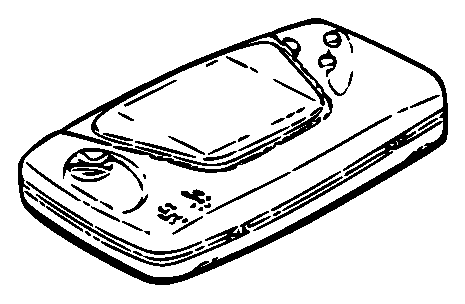
\includegraphics[width=20em]{SegaGameGear}}
\end{picture}

\newpage

\fancyfoot[L]{Sega Game Gear Hardware Reference Manual (Rev1) Page \thepage}

\renewcommand\contentsname{\uline{Table of Contents}}
\makeatletter
\renewcommand*{\@dotsep}{-2}
\makeatother
\tableofcontents

\newpage

\phantomsection
\section*{\scalebox{0.5}[1.0]{\uline{Precautions for Hardware}}}
\addcontentsline{toc}{section}{1. Precautions for Hardware}

\vspace{1.5em}

\phantomsection
\addcontentsline{toc}{subsection}{1. CPU clock}

\noindent 1. \ \ CPU clock\par
The CPU clock is 3.579545 MHz.\\

\phantomsection
\addcontentsline{toc}{subsection}{2. Memory area unusable area}

\noindent 2. \ \ Memory area unusable area\\
◎ \ \ DFF0H to DFFFH\par
When a ROM of 1 M or greater is used, the area for bank switching, and so on, is located\\
between FFF0H and FFFH. \ This area is used for reading (using images) bank data, so do not use it\\
as a normal work area. \ For this reason, it is necessary to set the stack pointer in such a way that\\
the stack does not use this area.\\
\par
\ \ \ Example: LD SP, 0DFF0H\\
\\
◎ \ \ E000H to FFFFH (excluding the area for bank switching, and so on)\par
This area contains the C000H to DFFFH RAM image. \ Do not access an image from this area but\\
from the C000H to DFFFH area instead.\\

\phantomsection
\addcontentsline{toc}{subsection}{3. VDP initialization}

\noindent 3. \ \ VDP initialization\par
Sometimes, when the power is switched ON, the reset of the CPU is canceled while the VDP\\
remains reset. \ In order to prevent this, confirm that the value of the V counter in the VDP has\\
become B0H and then access the data.\\
\\
Example:\par
\hskip 13em INIWAIT:\par
\hskip 17.5em IN \ \ \ \ \ A,(07EH) \ \ \ \ \ \ \ ; READ V-COUNTER\par
\hskip 17.5em CP \ \ \ \ \ 0B0H\par
\hskip 17.5em JP \ \ \ \ \ NZ,INIWAIT\par
\hskip 17.5em RET\\
\\

\phantomsection
\addcontentsline{toc}{subsection}{4. Interrupt}

\noindent 4. \ \ Interrupt\par
An interrupt is synchronized with the video timing (at the completion of the effective area\\
or at an arbitrary vertical position).\par
This interrupt uses the Z80 mode 1 interrupt, hence“IM 1"is executed at the beginning of the\\
program. \ A return from an interrupt routine is“RET"\hskip -0.5em.

\newpage

\phantomsection
\section*{\scalebox{0.5}[1.0]{\uline{System control port}}}
\addcontentsline{toc}{section}{2. System control port}

\noindent ☆ Indicates the state after a power-on reset.\\

\phantomsection
\addcontentsline{toc}{subsection}{① I/O port 00H (Read Only)  START/PAUSE button, region setting}

\noindent ① \ I/O port 00H (Read Only)

\vspace{-0.7em}
\setlength{\arrayrulewidth}{0.1em}
\setlength{\tabcolsep}{0.5em}
\renewcommand{\arraystretch}{2}
\hskip 2em \begin{tabular}{|l|c|c|c|c|c|c|c|}
\multicolumn{1}{c}{D7} & \multicolumn{1}{c}{D6} & \multicolumn{1}{c}{D5} & \multicolumn{1}{c}{D4} & \multicolumn{1}{c}{D3} & \multicolumn{1}{c}{D2} & \multicolumn{1}{c}{D1} & \multicolumn{1}{c}{D0}\\
\cline{1-8}
STT & NJAP & NNTS & * & * & * & * & *\\
\cline{1-8}
\end{tabular}

\vspace{1.2em}
\setlength{\arrayrulewidth}{0.1em}
\setlength{\tabcolsep}{0.5em}
\renewcommand{\arraystretch}{1}
\hskip 12em \begin{tabular}{|c|}
\multicolumn{1}{|c|}{ \ \ \ \ \ \ \ \ \ \ \ \ \ \ \ \ \ \ \ \ \ \ \ \ }\\
\hline
\end{tabular}

\vspace{1em}
\hskip 15em Meaningless\\
\\
○ \ \ STT\par
This is an input from the START/PAUSE button.\par
\ 0: Switch ON\par
\ 1: Switch OFF\\
○ \ \ NJAP\par
0: This is the domestic (Japan) mode.\par
1: This is the overseas mode.\\
○ \ \ NNTS\par
0: This is the NTSC mode.\par
1: This is the PAL mode.\\

\phantomsection
\addcontentsline{toc}{subsection}{② I/O port 01H (Read/Write) EXT connector}

\noindent ② \ I/O port 01H (Read/Write)

\vspace{-0.7em}
\setlength{\arrayrulewidth}{0.1em}
\setlength{\tabcolsep}{0.5em}
\renewcommand{\arraystretch}{2}
\hskip 2em \begin{tabular}{|c|l|l|l|l|l|l|l|}
\multicolumn{1}{c}{D7} & \multicolumn{1}{c}{D6} & \multicolumn{1}{c}{D5} & \multicolumn{1}{c}{D4} & \multicolumn{1}{c}{D3} & \multicolumn{1}{c}{D2} & \multicolumn{1}{c}{D1} & \multicolumn{1}{c}{D0}\\
\cline{1-8}
*& PC6 & PC5 & PC4 & PC3 & PC2 & PC1 & PC0 \\
\cline{1-8}
\end{tabular}

\vspace{2em}
This port is used to read/write data when the EXT connector is used as a 7-bit input/output\\
port. \ (The value after a power-on reset is indeterminate.)\\

\phantomsection
\addcontentsline{toc}{subsection}{③ I/O port 02H (Read/Write) NMI}

\noindent ③ \ I/O port 02H (Read/Write)

\vspace{-0.7em}
\setlength{\arrayrulewidth}{0.1em}
\setlength{\tabcolsep}{0.5em}
\renewcommand{\arraystretch}{2}
\hskip 2em \begin{tabular}{|c|c|c|c|c|c|c|c|}
\multicolumn{1}{c}{D7} & \multicolumn{1}{c}{D6} & \multicolumn{1}{c}{D5} & \multicolumn{1}{c}{D4} & \multicolumn{1}{c}{D3} & \multicolumn{1}{c}{D2} & \multicolumn{1}{c}{D1} & \multicolumn{1}{c}{D0}\\
\cline{1-8}
NINT & DPC6 & DPC5 & DPC4 & DPC3 & DPC2 & DPC1 & DPC0\\
\cline{1-8}
\end{tabular}

\vspace{2em}
\noindent ○ \ \ DPC6 to DPC0\par
0: PCx becomes the output.\\
\phantom \ \ ☆ 1: PCx becomes the input.\\
○ \ \ NINT\par
0: When PC6 is input, an NMI is generated at the fall of PC6.\\
\phantom \ \ ☆ 1: The above operation is disabled.\\
\par
\ ※Be sure to set the status of this port to“1"\hskip -0.5em. \ When using this value, first, set the status\\
to“1"after the first NMI is generated, then subsequently set it to“0"\hskip -0.5em.\\
If you fail to do this, the next NMI will not be generated.\\

\phantomsection
\addcontentsline{toc}{subsection}{④ I/O port 03H (Read/Write) Serial communications send data}

\noindent ④ \ I/O port 03H (Read/Write)

\vspace{-0.7em}
\setlength{\arrayrulewidth}{0.1em}
\setlength{\tabcolsep}{0.5em}
\renewcommand{\arraystretch}{2}
\hskip 2em \begin{tabular}{|l|l|l|l|l|l|l|l|}
\multicolumn{1}{c}{D7} & \multicolumn{1}{c}{D6} & \multicolumn{1}{c}{D5} & \multicolumn{1}{c}{D4} & \multicolumn{1}{c}{D3} & \multicolumn{1}{c}{D2} & \multicolumn{1}{c}{D1} & \multicolumn{1}{c}{D0}\\
\cline{1-8}
TD7 & TD6 & TD5 & TD4 & TD3 & TD2 & TD1 & TD0\\
\cline{1-8}
\end{tabular}

\vspace{1em}
\noindent ○ \ \ TD7 to TD0\par
Used to set the send data during serial communications.

\newpage

\phantomsection
\addcontentsline{toc}{subsection}{⑤ I/O port 04H (Read Only) Serial communications receive data}

\noindent ⑤ \ I/O port 04H (Read Only)

\vspace{-0.7em}
\setlength{\arrayrulewidth}{0.1em}
\setlength{\tabcolsep}{0.5em}
\renewcommand{\arraystretch}{2}
\hskip 2em \begin{tabular}{|l|l|l|l|l|l|l|l|}
\multicolumn{1}{c}{D7} & \multicolumn{1}{c}{D6} & \multicolumn{1}{c}{D5} & \multicolumn{1}{c}{D4} & \multicolumn{1}{c}{D3} & \multicolumn{1}{c}{D2} & \multicolumn{1}{c}{D1} & \multicolumn{1}{c}{D0}\\
\cline{1-8}
RD7 & RD6 & RD5 & RD4 & RD3 & RD2 & RD1 & RD0\\
\cline{1-8}
\end{tabular}

\vspace{2em}
\noindent ○ \ \ \ RD7 to RD0\par
The receive data is set during serial  communications.\\

\phantomsection
\addcontentsline{toc}{subsection}{⑥ I/O port 05H (Read/Write) Serial communications mode setting}

\noindent ⑥ \ I/O port 05H (Read/Write)\par
Serial communications mode setting

\vspace{-0.7em}
\setlength{\arrayrulewidth}{0.1em}
\setlength{\tabcolsep}{0.5em}
\renewcommand{\arraystretch}{2}
\hskip 2em \begin{tabular}{|l|l|l|l|l|c|c|c|}
\multicolumn{1}{c}{D7} & \multicolumn{1}{c}{D6} & \multicolumn{1}{c}{D5} & \multicolumn{1}{c}{D4} & \multicolumn{1}{c}{D3} & \multicolumn{1}{c}{D2} & \multicolumn{1}{c}{D1} & \multicolumn{1}{c}{D0}\\
\cline{1-8}
BS1 & BS0 & RON & TON & INT & FRER & RXRD & TXFL\\
\cline{1-8}
\end{tabular}

\vspace{2em}
\noindent ○ \ \ \ TXFL (Read)\\
\phantom \ \ ☆ 0: The next send data is written.\par
1: The send data cannot be written yet.\\
\\
○ \ \ \ RXRD (Read)\\
\\
\phantom \ \ ☆ 0: There is no receive data.\par
1: There is receive data.\\
\\
○ \ \ \ FRER (Read)\\
\phantom \ \ ☆ 0: There is no framing error.\par
1: There is a framing error.\\
\\
○ \ \ \ INT (Read/Write)\\
\phantom \ \ ☆ 0: The following operation is disabled.\par
1: An NMI is generated when data is received.\par
○ An operation such as that of I/O port 02H is unnecessary.\\
\\
○ \ \ \ TON (Read/Write)\\
\phantom \ \ ☆ 0: Sending is disabled.\par
1: Sending is enabled. \ (PC4 is forcibly made the output.)\\
\\
○ \ \ \ RON (Read/Write)\\
\phantom \ \ ☆ 0: Receive disable.\par
1: Receive enable. \ (PC5 is forcibly made the input.)\\
\\
○ \ \ \ BS1, BS0\par
\ Baud rate setting\\

\vspace{-0.5em}
\setlength{\arrayrulewidth}{0.1em}
\setlength{\tabcolsep}{0.5em}
\hskip 2em \begin{tabular}{c|c|c|l|}
\cline{2-4}
& BS1 & BS0 & \ Baud rate (bps) \ \ \ \ \\
\cline{2-4}
☆& 0 & 0 & 4800\\[-1.2em]
& 0 & 1 & 2400\\[-1.2em]
& 1 & 0 & 1200\\[-1.2em]
& 1 & 1 &  300\\
\cline{2-4}
\end{tabular}

\newpage

\phantomsection
\addcontentsline{toc}{subsection}{⑦ I/O port 06H (Write Only) Left-right distribution of sound}

\noindent ⑦ \ I/O port 06H (Write Only)\par
Left-right distribution of sound

\vspace{-0.7em}
\setlength{\arrayrulewidth}{0.1em}
\setlength{\tabcolsep}{0.5em}
\renewcommand{\arraystretch}{2}
\hskip 2em \begin{tabular}{|c|c|c|c|c|c|c|c|}
\multicolumn{1}{c}{D7} & \multicolumn{1}{c}{D6} & \multicolumn{1}{c}{D5} & \multicolumn{1}{c}{D4} & \multicolumn{1}{c}{D3} & \multicolumn{1}{c}{D2} & \multicolumn{1}{c}{D1} & \multicolumn{1}{c}{D0}\\
\cline{1-8}
NOSL & TN3L & TN2L & TN1L & NOSR & TN3R & TN2R & TN1R\\
\cline{1-8}
\end{tabular}

\vspace{2em}
\noindent ○ \ \ \ TN1R\par
0: The output of TONE 1 to the right is disabled.\\
\phantom \ \ ☆ 1: The output of TONE 1 to the right is enabled.\\
○ \ \ \ TN2R\par
0: The output of TONE 2 to the right is disabled.\\
\phantom \ \ ☆ 1: The output of TONE 2 to the right is enabled.\\
○ \ \ \ TN3R\par
0: The output of TONE 3 to the right is disabled.\\
\phantom \ \ ☆ 1: The output of TONE 3 to the right is enabled.\\
○ \ \ \ NOSR\par
0: The output of NOISE to the right is disabled.\\
\phantom \ \ ☆ 1: The output of NOISE to the right is enabled.\\
○ \ \ \ TN1L\par
0: The output of TONE 1 to the left is disabled.\\
\phantom \ \ ☆ 1: The output of TONE 1 to the left is enabled.\\
○ \ \ \ TN2L\par
0: The output of TONE 2 to the left is disabled.\\
\phantom \ \ ☆ 1: The output of TONE 2 to the left is enabled.\\
○ \ \ \ TN3L\par
0: The output of TONE 3 to the left is disabled.\\
\phantom \ \ ☆ 1: The output of TONE 3 to the left is enabled.\\
○ \ \ \ NOSL\par
0: The output of NOISE to the left is disabled.\\
\phantom \ \ ☆ 1: The output of NOISE to the left is enabled.\\

\phantomsection
\addcontentsline{toc}{subsection}{⑧ I/O port 30H, 31H (Read Only) Loader access (development board only)}

\noindent ⑧ \ Loader access (development board only)

\vspace{-0.7em}
\setlength{\arrayrulewidth}{0.1em}
\setlength{\tabcolsep}{0.5em}
\renewcommand{\arraystretch}{2}
\hskip 2em \begin{tabular}{|l|l|l|l|l|l|l|l|l}
\multicolumn{1}{c}{D7} & \multicolumn{1}{c}{D6} & \multicolumn{1}{c}{D5} & \multicolumn{1}{c}{D4} & \multicolumn{1}{c}{D3} & \multicolumn{1}{c}{D2} & \multicolumn{1}{c}{D1} & \multicolumn{1}{c}{D0} &\\
\cline{1-8}
LD7 & LD6 & LD5 & LD4 & LD3 & LD2 & LD1 & LD0 & \ I/O port 30H (Read)\\
\cline{1-8}
\end{tabular}

\vspace{2em}
\noindent ○ \ \ LD7 - LD0\par
8-bit data which is read from the printer port

\vspace{-0.7em}
\setlength{\arrayrulewidth}{0.1em}
\setlength{\tabcolsep}{0.5em}
\renewcommand{\arraystretch}{2}
\hskip 2em \begin{tabular}{|c|c|c|c|c|l|c|c|l}
\multicolumn{1}{c}{D7} & \multicolumn{1}{c}{D6} & \multicolumn{1}{c}{D5} & \multicolumn{1}{c}{D4} & \multicolumn{1}{c}{D3} & \multicolumn{1}{c}{D2} & \multicolumn{1}{c}{D1} & \multicolumn{1}{c}{D0} &\\
\cline{1-8}
0 & 0 & 0 & 0 & 0 & CLR & BUSY & NSTB & \ I/O port 31H (Read)\\
\cline{1-8}
\end{tabular}

\vspace{2em}
\noindent ○ \ \ NSTB\par
STROBE signal input (active Low)\\
○ \ \ BUSY\par
BUSY signal input (active High)\\
○ \ \ CLR\par
\ Loader clear button input (active Low)\par
When this button is pressed, LD7 to LD0 all become“0"\hskip -0.5em, the ACK signal becomes High, and the\\
BUSY signal becomes Low.

\newpage

\setlength{\arrayrulewidth}{0.1em}
\setlength{\tabcolsep}{0.5em}
\renewcommand{\arraystretch}{2}
\hskip 2em \begin{tabular}{|c|c|c|c|c|c|c|l|l}
\multicolumn{1}{c}{D7} & \multicolumn{1}{c}{D6} & \multicolumn{1}{c}{D5} & \multicolumn{1}{c}{D4} & \multicolumn{1}{c}{D3} & \multicolumn{1}{c}{D2} & \multicolumn{1}{c}{D1} & \multicolumn{1}{c}{D0} &\\
\cline{1-8}
* & * & * & * & * & * & * & ACK & \ I/O port 30H (Write)\\
\cline{1-8}
\end{tabular}

\vspace{2em}
\noindent ○ \ \ ACK\par
0: The ACK signal becomes High.\par
1: The Ack signal becomes Low (active).\\
\\
※ \ \ When the strobe signal falls, eight bits of data are latched, and simultaneously the BUSY\\
signal automatically becomes High. \ Once the data has been read, the ACK signal is made Low,\\
then High once again. \ The BUSY signal automatically becomes Low. \ The LED lights when the BUSY\\
signal becomes High.\\

\phantomsection
\addcontentsline{toc}{subsection}{⑨ I/O port DCH, DDH (Read Only) JOYSTICK board}

\noindent ⑨ \ \ JOYSTICK board (Read Only)

\vspace{-0.7em}
\setlength{\arrayrulewidth}{0.1em}
\setlength{\tabcolsep}{0.5em}
\renewcommand{\arraystretch}{2}
\hskip 2em \begin{tabular}{|r|r|r|r|r|r|r|r|l}
\multicolumn{1}{c}{D7} & \multicolumn{1}{c}{D6} & \multicolumn{1}{c}{D5} & \multicolumn{1}{c}{D4} & \multicolumn{1}{c}{D3} & \multicolumn{1}{c}{D2} & \multicolumn{1}{c}{D1} & \multicolumn{1}{c}{D0} &\\
\cline{1-8}
DWE & UPE & TR1 & TL1 & RI1 & LE1 & DW1 & UP1 & \ \ I/O port DCH\\
\cline{1-8}
\end{tabular}

\vspace{1em}
\setlength{\arrayrulewidth}{0.1em}
\setlength{\tabcolsep}{0.5em}
\renewcommand{\arraystretch}{2}
\hskip 2em \begin{tabular}{|r|c|c|c|r|r|r|r|l}
\multicolumn{1}{c}{D7} & \multicolumn{1}{c}{D6} & \multicolumn{1}{c}{D5} & \multicolumn{1}{c}{D4} & \multicolumn{1}{c}{D3} & \multicolumn{1}{c}{D2} & \multicolumn{1}{c}{D1} & \multicolumn{1}{c}{D0} &\\
\cline{1-8}
THE & * & * & * & TRE & TLE & RIE & LEE & \ \ I/O port DDH\\
\cline{1-8}
\end{tabular}

\vspace{2em}
\noindent ※ UP1-1P UP switch \ \ \ \ \ \ \ \ \ \ \ \ \ UPE-EXT UP switch\\
\phantom \ \ \ DW1-1P DOWN switch \ \ \ \ \ \ \ \ \ \ \ DWE-EXT DOWN switch\\
\phantom \ \ \ LE1-1P LEFT switch \ \ \ \ \ \ \ \ \ \ \ LEE-EXT LEFT switch\\
\phantom \ \ \ RI1-1P RIGHT switch \ \ \ \ \ \ \ \ \ \ RIE-EXT RIGHT switch\\
\phantom \ \ \ TL1-1P TRIGGER left button \ \ \ TLE-EXT TRIGGER left button\\
\phantom \ \ \ TR1-1P TRIGGER right button \ \ TRE-EXT TRIGGER right button\\
\phantom \ \ \ \ \ \ \ \ \ \ \ \ \ \ \ \ \ \ \ \ \ \ \ \ \ \ \ \ \ \ \ \ \ THE-EXT (Same as PC6 input)\\
\\
One bit is read to port as“1"when either there is nothing connected to the terminal or the\\
corresponding switch is not pressed, and is read as“0"when the switch is pressed.

\newpage

\phantomsection
\section*{\scalebox{0.5}[1.0]{\uline{Material}}\\
\scalebox{0.5}[1.0]{\uline{Using the ROM bank switching and backup RAM}}}

\addcontentsline{toc}{section}{3. Material: Using the ROM bank switching and backup RAM}

\noindent In this model, the capacity of the memory can vary between 1 and 4 Megabits by bank switching.\\
\\
Note:\\
\phantom \ \ Area 0: 0000 to 3FFF\\
\phantom \ \ Area 1: 4000 to 7FFF\\
\phantom \ \ Area 2: 8000 to BFFF\\
\\
The size of one bank is 16 Kbyte. \ The banks are arranged sequentially in the ROM without\\
overlapping.\\

\phantomsection
\addcontentsline{toc}{subsection}{A. When the memory capacity is 1 Megabit}

\noindent A. \ \ When the memory capacity is 1 Megabit\\
Area 0 is fixed to bank 0 (first 16 KBytes of the ROM), and area 1 is fixed to bank 1.\\
Area 2 enables the banks to be switched over by setting a value in register FFFFH.

\vspace{0.5em}
\setlength{\arrayrulewidth}{0.1em}
\setlength{\tabcolsep}{0.5em}
\renewcommand{\arraystretch}{2}
\hskip 1em \begin{tabular}{|c|c|c|c|c|c|c|c|l}
\multicolumn{1}{l}{D7} & \multicolumn{1}{l}{D6} & \multicolumn{1}{l}{D5} & \multicolumn{1}{l}{D4} & \multicolumn{1}{l}{D3} & \multicolumn{1}{l}{D2} & \multicolumn{1}{l}{D1} & \multicolumn{1}{l}{D0} &\\
\cline{1-8}
 0  &  0  &  0  &  0  &  0  & 1/0 & 1/0 & 1/0 & \ \ \ \ FFFFH\\
\cline{1-8}
\end{tabular}

\vspace{2em}
\noindent For bank 0, set 00H (same bank as for area 0).\\
For bank 7, set 07H.\\

\phantomsection
\addcontentsline{toc}{subsection}{B. If the capacity is 2 MBytes or more, or a backup RAM is provided}

\noindent B. \ \ If the capacity is 2 MBytes or more, or a backup RAM is provided\\

\phantomsection
\addcontentsline{toc}{subsubsection}{① Bank control register (FFFCH)}

\noindent ① \ \ Bank control register (FFFCH)

\vspace{-0.7em}
\setlength{\arrayrulewidth}{0.1em}
\setlength{\tabcolsep}{0.5em}
\renewcommand{\arraystretch}{2}
\hskip 1em \begin{tabular}{|c|c|c|c|c|c|c|c|l}
\multicolumn{1}{l}{D7} & \multicolumn{1}{l}{D6} & \multicolumn{1}{l}{D5} & \multicolumn{1}{l}{D4} & \multicolumn{1}{l}{D3} & \multicolumn{1}{l}{D2} & \multicolumn{1}{l}{D1} & \multicolumn{1}{l}{D0} &\\
\cline{1-8}
0/1 &  0  &  0  &  0  & 0/1 &  0  & 1/0 & 1/0 & \ \ \ \ FFFCH\\
\cline{1-8}
\end{tabular}

\vspace{1em}
\setlength{\arrayrulewidth}{0.1em}
\setlength{\tabcolsep}{0.5em}
\renewcommand{\arraystretch}{1}
\hskip 3em \begin{tabular}{ccccccccl}
\multicolumn{1}{|c}{   } & \multicolumn{1}{c}{   } & \multicolumn{1}{c}{   } & \multicolumn{1}{|c}{   } & \multicolumn{1}{|c}{   } & \multicolumn{1}{c}{   } & \multicolumn{1}{|c}{   } & \multicolumn{1}{|c}{ } &\\[-0.4em]
\multicolumn{1}{|c}{} & \multicolumn{1}{c}{} & \multicolumn{1}{c}{} & \multicolumn{1}{|c}{} & \multicolumn{1}{|c}{} & \multicolumn{1}{c}{} & \multicolumn{1}{|c}{} & \multicolumn{1}{|c}{} & \ \ Bank number offset\\[-0.8em]
\cline{7-8}
\multicolumn{1}{|c}{} & \multicolumn{1}{c}{} & \multicolumn{1}{c}{} & \multicolumn{1}{|c}{} & \multicolumn{1}{|c}{} & \multicolumn{1}{c}{} & \multicolumn{1}{c}{} & \multicolumn{1}{c}{} &\\[-0.4em]
\multicolumn{1}{|c}{} & \multicolumn{1}{c}{} & \multicolumn{1}{c}{} & \multicolumn{1}{|c}{} & \multicolumn{1}{|c}{} & \multicolumn{1}{c}{} & \multicolumn{1}{c}{} & \multicolumn{1}{c}{} & \ \ ROM/external RAM selection\\[-0.8em]
\cline{5-8}
\multicolumn{1}{|c}{} & \multicolumn{1}{c}{} & \multicolumn{1}{c}{} & \multicolumn{1}{|c}{} & \multicolumn{1}{c}{} & \multicolumn{1}{c}{} & \multicolumn{1}{c}{} & \multicolumn{1}{c}{} &\\[-0.4em]
\multicolumn{1}{|c}{} & \multicolumn{1}{c}{} & \multicolumn{1}{c}{} & \multicolumn{1}{|c}{} & \multicolumn{1}{c}{} & \multicolumn{1}{c}{} & \multicolumn{1}{c}{} & \multicolumn{1}{c}{} & \ \ Work RAM selection\\[-0.8em]
\cline{4-8}
\multicolumn{1}{|c}{} & \multicolumn{1}{c}{} & \multicolumn{1}{c}{} & \multicolumn{1}{c}{} & \multicolumn{1}{c}{} & \multicolumn{1}{c}{} & \multicolumn{1}{c}{} & \multicolumn{1}{c}{} &\\[-0.4em]
\multicolumn{1}{|c}{} & \multicolumn{1}{c}{} & \multicolumn{1}{c}{} & \multicolumn{1}{c}{} & \multicolumn{1}{c}{} & \multicolumn{1}{c}{} & \multicolumn{1}{c}{} & \multicolumn{1}{c}{} & \ \ Write Protect\\[-0.8em]
\cline{1-8}
\end{tabular}

\vspace{2em}
\noindent ○ \ Bank number offset\\
All of the banks for areas 0 to 2 area shifted by 1 bank group (8 banks) \ time the value 1 to 3 is\\
set here. If an offset number causes a bank number to exceed 1FH(31), it goes Bank 0. The value set\\
here will become valid when it is subsequently set in one of bank registers 0 to 2.\\
\\
○ \ Switching between ROM/external RAM\\
When 0: The ROM (bank) is assigned to area 2.\\
When 1: The external RAM is assigned to area 2 (when an extrenal RAM exists).\\
\\
○ \ Work RAM selection\\
If 1 is set here, normal access to the work RAM (C000H to DFFFH) of the main body will be prevented.\\
\phantom \ \ Be sure, therefore, to set 0.\\
\\
○ \ WRITE PROTECT\\
If 1 is set here when the development RAM board is used, data re-write will not take place.\\
Set 0 in mass-production machines.

\newpage

\phantomsection
\addcontentsline{toc}{subsubsection}{② Bank register 0 (FFFDH)}

\noindent ② \ Bank register 0 (FFFDH)\par
0000H to 03FFH of area 0 is fixed to bank 0. \ Bank selection of other areas can be performed\\
by setting a value at FFFDH.

\vspace{0.5em}
\setlength{\arrayrulewidth}{0.1em}
\setlength{\tabcolsep}{0.5em}
\renewcommand{\arraystretch}{2}
\hskip 1em \begin{tabular}{|c|c|c|c|c|c|c|c|l}
\multicolumn{1}{l}{D7} & \multicolumn{1}{l}{D6} & \multicolumn{1}{l}{D5} & \multicolumn{1}{l}{D4} & \multicolumn{1}{l}{D3} & \multicolumn{1}{l}{D2} & \multicolumn{1}{l}{D1} & \multicolumn{1}{l}{D0} &\\
\cline{1-8}
 0  &  0  &  0  & 0/1 & 0/1 & 1/0 & 1/0 & 1/0 & \ \ \ \ FFFDH\\
\cline{1-8}
\end{tabular}

\vspace{1em}
For bank 00: Set 00H.\par
For bank 1F: Set 1FH.\\

\phantomsection
\addcontentsline{toc}{subsubsection}{③ Bank register 1 (FFFEH)}

\noindent ③ \ Bank register 1 (FFFEH)\par
A bank selection can be performed in area 1 by setting a value in FFFEH.

\vspace{0.5em}
\setlength{\arrayrulewidth}{0.1em}
\setlength{\tabcolsep}{0.5em}
\renewcommand{\arraystretch}{2}
\hskip 1em \begin{tabular}{|c|c|c|c|c|c|c|c|l}
\multicolumn{1}{l}{D7} & \multicolumn{1}{l}{D6} & \multicolumn{1}{l}{D5} & \multicolumn{1}{l}{D4} & \multicolumn{1}{l}{D3} & \multicolumn{1}{l}{D2} & \multicolumn{1}{l}{D1} & \multicolumn{1}{l}{D0} &\\
\cline{1-8}
 0  &  0  &  0  & 0/1 & 0/1 & 1/0 & 1/0 & 1/0 & \ \ \ \ FFFEH\\
\cline{1-8}
\end{tabular}

\vspace{1em}
For bank 00: Set 00H.\par
For bank 1F: Set 1FH.\\

\phantomsection
\addcontentsline{toc}{subsubsection}{④ Bank register 2 (FFFFH)}

\noindent ④ \ Bank register 2 (FFFFH)\par
A bank selection can be performed in area 2 by setting a value in FFFFH.

\vspace{0.5em}
\setlength{\arrayrulewidth}{0.1em}
\setlength{\tabcolsep}{0.5em}
\renewcommand{\arraystretch}{2}
\hskip 1em \begin{tabular}{|c|c|c|c|c|c|c|c|l}
\multicolumn{1}{l}{D7} & \multicolumn{1}{l}{D6} & \multicolumn{1}{l}{D5} & \multicolumn{1}{l}{D4} & \multicolumn{1}{l}{D3} & \multicolumn{1}{l}{D2} & \multicolumn{1}{l}{D1} & \multicolumn{1}{l}{D0} &\\
\cline{1-8}
 0  &  0  &  0  & 0/1 & 0/1 & 1/0 & 1/0 & 1/0 & \ \ \ \ FFFFH\\
\cline{1-8}
\end{tabular}

\vspace{1em}
For bank 00: Set 00H.\par
For bank 1F: Set 1FH.\\
\\
Caution:\\
The above registers are not initialized when the power is switched on. \ For this reason, be sure\\
to initialize them program in 0 to 3FFFH.. \ (The first 1 KByte is fixed for this purpose.)\\
Sometimes, the work RAM cannot be accessed normally, hence the work RAM (and also sub-routines, )\\
are allowed to be used after this initialization. \ When using a backup RAM, do not use the first and\\
last addresses because there is a possibility of the data being changed when the power\\
is switched on.\\
\\
Example:\par
\hskip 5.5em ORG \ \ \ \ \ \ 00000H\par
\hskip 5.5em DI\par
\hskip 5.5em IM \ \ \ \ \ 1\par
\hskip 5.5em LD \ \ \ \ \ SP,0DFF0H\\
\par
\hskip 5.5em LD \ \ \ \ \ A,000H\par
\hskip 5.5em LD \ \ \ \ \ (0FFFCH),A\par
\hskip 5.5em LD \ \ \ \ \ A,000H\par
\hskip 5.5em LD \ \ \ \ \ (0FFFDH),A\par
\hskip 5.5em LD \ \ \ \ \ A,001H\par
\hskip 5.5em LD \ \ \ \ \ (0FFFEH),A\par
\hskip 5.5em LD \ \ \ \ \ A,002H\par
\hskip 5.5em LD \ \ \ \ \ (0FFFFH),A\par

\newpage

\phantomsection
\section*{\scalebox{0.5}[1.0]{\uline{Material MAPPING}}}
\addcontentsline{toc}{section}{4. Material: MAPPING}

\phantomsection
\addcontentsline{toc}{subsection}{MEMORY MAP, I/O MAP}

\hskip 2.5em MEMORY MAP \hskip 15em I/O MAP

\vspace{0.5em}
\setlength{\arrayrulewidth}{0.1em}
\setlength{\tabcolsep}{0.5em}
\noindent
\hskip -0.5em \begin{tabular}{r|l|r|l|}
\multicolumn{1}{c}{0000} & \multicolumn{1}{c}{} & \multicolumn{1}{r}{00} & \multicolumn{1}{c}{}\\[-3.6em]
\multicolumn{1}{c}{} & \multicolumn{1}{c}{} & \multicolumn{1}{r}{} & \multicolumn{1}{c}{}\\
\cline{2-2}
\cline{4-4}
& Cartridge \ \ \ \ \ \ \ \ \ \ \ \ \ \ \ \ \ \ \ & \ \ \ \ \ \ \ \ \ \ \ \ \ \ \ \ \ \ \ & 00,01,02,03,04,05 and 06\\[-1.2em]
& & & : Used with system control. \ \\[4em]
& Area 0 & &\\[-1.2em]
4000 & & 40 &\\[-1.2em]
\cdashline{2-2}[3pt/3pt]
\cdashline{4-4}[3pt/3pt]
& Cartridge & & 7E -{-} Read\\[-1.2em]
& & & \ \ \ \ \ \ : V counter\\[-1.2em]
& & & 7F -{-} Read\\[-1.2em]
& & & \ \ \ \ \ \ : H counter\\[-1.2em]
& & & 7F -{-} Write\\[-1.2em]
& & & \ \ \ \ \ \ : PSG\\[-1.2em]
& Area 1 & &\\[-1.2em]
8000 & & 80 &\\[-1.2em]
\cdashline{2-2}[3pt/3pt]
\cdashline{4-4}[3pt/3pt]
& Cartridge & & \ BE and BF\\[-1.2em]
& & & \ : Used with VDP\\[4em]
& Area 2 & &\\[-1.2em]
C000 & & C0 &\\[-1.2em]
\cdashline{2-2}[3pt/3pt]
\cdashline{4-4}[3pt/3pt]
& 8 Kbyte work RAM & & \ DC and DD\\[-1.2em]
& & & \ : Used as JOYSTICK inputs.\\
E000 & & &\\[-1.2em]
\cdashline{2-2}[3pt/3pt]
& Top image & &\\[1.2em]
FFFF & & FF &\\[-1.2em]
\cline{2-2}
\cline{4-4}
\end{tabular}

\vspace{2em}
Never access data using an image address.

\newpage

\phantomsection
\section*{\scalebox{0.5}[1.0]{\uline{Supplementary description for manual}}}
\addcontentsline{toc}{section}{5. Supplementary description for manual}

\phantomsection
\addcontentsline{toc}{subsection}{A. System control port}

\noindent A. \ \ System control port

\phantomsection
\addcontentsline{toc}{subsubsection}{③ I/O port 02H (Read/Write) NMI}

\noindent \ ③ I/O port 02H (Read/Write)\par
{*} Normally, be sure to make the status of this port“1"\hskip -0.5em. \ When using this value, first,\\
set the status to“1"after the first NMI is generated, then subsequently set it to“0"\hskip -0.5em.\\
If you fail to do this, the next NMI will not be generated.\\
\\
\uline{Addition:}\par
An NMI is enabled after the execution of one command from when the port is set to“0"\hskip -0.5em.\\
This is to prevent the NMI from becoming active once again in the NMI routine.\\
Normally, therefore, perform the following processing.\\
\par
\hskip 3.5em NMI:\par
\hskip 5.5em .\par
\hskip 5.5em .\par
\hskip 5.5em .\par
\hskip 5.5em .\par
\hskip 5.5em LD \ \ \ \ \ A,11XXXXXXB\par
\hskip 5.5em OUT \ \ \ \ (002H),A\par
\hskip 5.5em LD \ \ \ \ \ A,01XXXXXXB\par
\hskip 5.5em OUT \ \ \ \ (002H),A\par
\hskip 5.5em RETN \ \ \ \ \ \ \ \ \ \ \ \ \ \ \ \ \ \ \ ; An NMI is enabled after this command.\\
\\

\phantomsection
\addcontentsline{toc}{subsection}{B. System control port}

\noindent B. \ \ System control port

\phantomsection
\addcontentsline{toc}{subsubsection}{⑥ I/O port 05H (Read/Write) Serial communications mode setting}

\noindent \ ⑥ I/O port 05H (Read/Write)\par
Mode setting for serial communications\\
\\
{*} INT\\
{*} \ \ \ There is no need to perform an operation such as that of I/O port 02H.\\
\\
\uline{Addition:}\par
When using this function (serial communications NMI), set NINT of I/O port 02H to the disable\\
state (\hskip -0.5em“1"\hskip -0.5em). \ An NMI will be generated at the fall of the pulse at the NMI terminal.\\
If, however, a serial communications NMI is generated, the NMI terminal will go LOW, preventing the\\
next NMI from becoming active. \ The NMI terminal is made HIGH as a result of reading the data of I/O\\
port 04H, so read the data each time an NMI is generated. \ If it is conceivable that the NMI\\
terminal may already be LOW at the start of the communications, perform a“dummy"read operation\\
once.\\

\phantomsection
\addcontentsline{toc}{subsection}{C. System control port}

\noindent C. \ \ System control port\\

\phantomsection
\addcontentsline{toc}{subsubsection}{⑦ I/O port 06H (Write Only) Left-right distribution of sound}

\noindent \ ⑦ I/O port 06H (Write Only)\par
Left-right distribution of sound Supplementary explanation. \ When the headphones are plugged in,\\
the output from the speaker is cut off and instead the sound will be heard in stereo from the\\
headphones. \ When the earphones are not plugged in, the sound will be heard from the speaker in\\
monaural. \ In the latter case, the distribution of the sound from all channels (three tones \& noise)\\
\phantom \ will be enabled. \ If the output from the left and right channels was disabled not by attenuator\\
control but by distribution, the sound will not be heard from the headphones but will be heard from\\
the speaker. \ To turn off both the left and right channels of the speaker, use the PSG,\\
by PSG side control.

\newpage

\phantomsection
\addcontentsline{toc}{subsection}{D. Communications}

\noindent D. \ \ Communications

\phantomsection
\addcontentsline{toc}{subsubsection}{① Connecting the communications cable}

\noindent \ ① Connecting the communications cable Cross-connect the game gear communications cable as shown\\
below.\\
\par
\hskip 2em Communications connector

\vspace{0.5em}
\setlength{\arrayrulewidth}{0.1em}
\setlength{\tabcolsep}{0.5em}
\renewcommand{\arraystretch}{2}
\hskip 5em \begin{tabular}{|r|l|cl}
\cline{1-2}
1 & PC0 & \ \ \ ━━━━━ & To opposite side PC2\\
\cline{1-2}
2 & PC1 & \ \ \ ━━━━━ & To opposite side PC3\\
\cline{1-2}
3 & PC2 & \ \ \ ━━━━━ & To opposite side PC0\\
\cline{1-2}
4 & PC3 & \ \ \ ━━━━━ & To opposite side PC1\\
\cline{1-2}
5 & +5V & &\\
\cline{1-2}
6 & PC4 & \ \ \ ━━━━━ & To opposite side PC5\\
\cline{1-2}
7 & PC6 & \ \ \ ━━━━━ & To opposite side PC6\\
\cline{1-2}
8 & GND & \ \ \ ━━━━━ & To opposite side GND\\
\cline{1-2}
9 & PC5 & \ \ \ ━━━━━ & To opposite side PC4\\
\cline{1-2}
10 & NC & &\\
\cline{1-2}
\end{tabular}

\vspace{2em}

\phantomsection
\addcontentsline{toc}{subsubsection}{② Parallel communications}

\noindent \ ② Parallel communications\par
PC0 to PC6 can be set to an arbitrary input or output by means of the control register of the\\
I/O port. \ Be sure to set the connecting terminals so that the terminal on one side is the output,\\
and that on the opposite side is the input. \ (Never make the terminals on both sides the output.)\\
In the case of parallel communications, control the exchange of data either by polling using\\
software (check the data), or by applying an interrupt (NMI) using PC6. \ When applying an NMI using\\
PC6, however, it is necessary to take noise into account because an NMI will be generated by\\
a momentary change in PC6.\\

\phantomsection
\addcontentsline{toc}{subsubsection}{③ Serial communications}

\noindent \ ③ Serial communications\par
Serial communications can be performed in one of two single directions, from PC4 (output from\\
one'\hskip -0.5ems own side) -> PC5 (input to opposite side), or from PC5 (input to one'\hskip -0.5ems own side) <- PC4\\
(output from opposite side). \ Serial and parallel conversion and interrupt (NMI) generation\\
(when data is received) accompanying the receiving or sending of data take place automatically when\\
the hardware is connected to these terminals. \ To perform serial communications, set TON and RON of\\
I/O port 05H to“1"\hskip -0.5em. \ By doing this, PC4 will automatically become the output, and PC5 the input.\\
These settings will take priority over the PC4 and PC5 input/output settings. \ Bits other than those\\
of PC4 and PC5 will become the settings of I/O port 02H. \ (Like (2), never make both terminals the\\
output.) \ When performing serial communications only, be sure to set NINT of I/O port 02H to prevent\\
PC6 from generating an NMI.

\newpage

\phantomsection
\addcontentsline{toc}{subsubsection}{④ Coexistence of parallel and serial communications}

\noindent \ ④ Coexistence of parallel and serial communications\par
When performing serial communications, PC4 and PC5 are used to send and receive serial data.\\
Parallel communications can be performed using the bits other than these. \ An NMI can be generated\\
by PC6 and also by receiving of serial data. \ In the former case, care must be taken because PC6\\
does not have a data receiving flag such as the serial RXRD. \ The blocks of the circuit used to\\
generate these NMI are shown below.\\
\\
\par
\hskip 15em Flip-flop for parellel communication

\vspace{0.5em}
\setlength{\arrayrulewidth}{0.1em}
\setlength{\tabcolsep}{0.5em}
\renewcommand{\arraystretch}{2}
\hskip 2.5em \begin{tabular}{lc|l|cclc|l|}
\cline{3-3}
\cline{8-8}
\ \ \ PC6 \ \ \ \ \ \ \ \ \ \ \ \ \ \ \ \ \ \ & & SET \ \ \ & \ \ \ \ \ & \ \ \ \ \ & \ \ \ \ \ \ \ \ \ & \ \ \ \ \ \ \ & \ \ \ \ \ \\[-1.2em]
\cline{2-2}
& & & & & & & Z80\\[-3.6em]
& & & & & & &\\
\cline{4-4}
\ \ \ NINT & & RESET & \multicolumn{1}{c|}{} & & & &\\[-3.6em]
& & & \multicolumn{1}{c|}{} & & & &\\
\cline{2-2}
\cline{6-6}
& & & \multicolumn{1}{c|}{} & \multicolumn{1}{c|}{} & \multicolumn{1}{l|}{OR and} & &\\[-1.2em]
\cline{3-3}
\cline{5-5}
& \multicolumn{1}{c}{} & \multicolumn{1}{c}{} & & \multicolumn{1}{c|}{} & \multicolumn{1}{l|}{inverted} & & NMI\\[-1.2em]
\cline{7-7}
& \multicolumn{1}{c}{} & \multicolumn{1}{c}{} & & \multicolumn{1}{c|}{} & \multicolumn{1}{l|}{output} & &\\[-3.6em]
& \multicolumn{1}{c}{} & \multicolumn{1}{c}{} & & \multicolumn{1}{c|}{} & \multicolumn{1}{l|}{} & &\\
\cline{3-3}
\cline{5-5}
Receiving of serial data & & SET & \multicolumn{1}{c|}{} & \multicolumn{1}{c|}{} & \multicolumn{1}{l|}{} & &\\[-1.2em]
\cline{2-2}
\cline{6-6}
& & & \multicolumn{1}{c|}{} & & & &\\[-1.2em]
\cline{4-4}
Reading of serial data & & RESET & & & & &\\[-1.2em]
\cline{2-2}
& & & & & & &\\[-1.2em]
\cline{3-3}
\cline{8-8}
\end{tabular}

\vspace{0.7em}

\hskip 15.5em Flip-flop for serial communication\\
\par
\ An NMI is generated when one of the two reset flip-flops is set. \ (This is because an NMI is\\
generated not when the pulse level is LOW but when the pulse falls.) \ It should be appreciated that\\
it is necessary to reset the set flip-flop so that the next NMI can be generated.\\
\\
\begin{center}
- END - \ \ \ \ \ \ \
\end{center}

\newpage

\phantomsection
\section*{\scalebox{0.5}[1.0]{\uline{VDP Manual}}}
\addcontentsline{toc}{section}{6. VDP Manual}

\vspace{1em}

\phantomsection
\addcontentsline{toc}{subsection}{(1) GAME GEAR FEATURES}

\noindent (1) \ GAME GEAR FEATURES\\
{*} \ \ \ 16-kbyte VRAM\\
\\
{*} \ \ \ Scroll SCREEN: Horizontal 20 cells x vertical 18 cells (one cell = 8 x 8 dots)\\
The virtual area is 32 cells in the horizontal direction x 28 cells in the vertical direction,\\
permitting smooth scrolling in the horizontal and vertical directions.\\
\\
{*} \ \ \ The scroll screen can be left-right reversed, and up-down reversed, and also its priority with\\
respect to sprites can be selected.\\
\\
{*} \ \ \ 64 colors out of a total of 4096 colors can be displayed for each dot of the scroll\\
surface. By designating a palette for each cell, two kinds of 16-color groups can be selected.\\
\\
{*} \ \ \ Sixteen sprites (movable objects) can be displayed on a single screen. \ Up to eight sprites of\\
either 8 x 8 dots or 8 x 16 dots (vertical) in size can be selected on the same horizontal line.\\
\\
\phantom \ {*} \ \ \ Sixteen colors out of a total of 4096 can be displayed for each dot of a sprite.\\
\\
{*} \ \ \ The maximum number of character pattern definitions (8 x 8 dots) is 448 for both the scroll\\
surface and sprites (256 of these are used for sprites, however this is reduced to 128 for 8 x 16\\
sprites).


\newpage

\phantomsection
\addcontentsline{toc}{subsection}{(2) Effective area and LCD display area}

\noindent (2) \ Effective area and LCD display area\par
This VDP was initially designed on the basis of a TV (NTSC) format, hence only a portion of the\\
picture created by the VDP is displayed on the LCD. \ This relationship is shown in the figure below.\\

\vspace{0.5em}
\setlength{\arrayrulewidth}{0.1em}
\setlength{\tabcolsep}{0.5em}
\renewcommand{\arraystretch}{2}
\hskip 1em \begin{tabular}{|l|l|l|cc|l}
\cline{1-3}
\cline{5-5}
\multicolumn{3}{|l|}{\ TOP BORDER \ \ \ \ \ \ \ \ \ \ \ \ \ \ \ \ \ \ \ \ \ \ \ \ \ \ \ \ \ \ \ \ ↑} & & &\\[-1.2em]
\multicolumn{3}{|l|}{\ \ \ \ \ \ \ \ \ \ \ \ \ \ \ \ \ \ \ \ \ \ \ \ \ \ \ \ \ \ \ \ \ \ \ \ \ \ Equivalent to 27 lines} & & &\\[-1.2em]
\multicolumn{3}{|l|}{\ \ \ \ \ \ \ \ \ \ \ \ \ \ \ \ \ \ \ \ \ \ \ \ \ \ \ \ \ \ \ \ \ \ \ \ \ \ \ \ \ \ \ \ ↓} & & &\\
\cline{1-3}
\multicolumn{3}{|l|}{\ \ \ \ \ \ \ \ \ \ \ \ \ \ \ \ \ \ \ \ \ \ \ \ \ \ \ \ \ \ \ \ \ \ \ \ \ \ \ \ \ \ \ \ ↑} & & &\\[-1.2em]
\multicolumn{3}{|l|}{Effective area (original TV display) \ \ \ \ \ \ 3 cells} & & &\\[-1.2em]
\multicolumn{3}{|l|}{\ \ \ \ \ \ \ \ \ \ \ \ \ \ \ \ \ \ \ \ \ \ \ \ \ \ \ \ \ \ \ \ \ \ \ \ \ \ \ \ \ \ \ \ ↓} & & &\\
\cline{2-2}
←6cells→ & LCD display area \ \ \ \ \ \ \ \ \ \ \ \ \ \ \ \ \ \ \ \ \ \ & ←6cells→ & & &\\[-1.2em]
& ( 20 cells (horizontal) & & & &\\[-1.2em]
& \ \ \ \ \ \ \ \ x 18 cells (vertical)) & & & &\\[-1.2em]
& & & & &\\[-1.2em]
& & & & &\\[-1.2em]
& & & & & 1 Frame\\[-1.2em]
& & & & & \ (60 times per second)\\[-1.2em]
& & & & &\\[-1.2em]
& & & & &\\[-1.2em]
& & & & &\\[-1.2em]
& & & & &\\[-1.2em]
\cline{2-2}
\multicolumn{3}{|l|}{\ \ \ \ \ \ \ \ \ \ \ \ \ \ \ \ \ \ \ \ \ \ \ \ \ \ \ \ \ \ \ \ \ \ \ \ \ \ \ \ \ \ \ \ ↑} & & &\\[-1.2em]
\multicolumn{3}{|l|}{\ \ \ \ \ \ \ \ \ \ \ \ \ \ \ \ \ \ \ \ \ \ \ \ \ \ \ \ \ \ \ \ \ \ \ \ \ \ \ \ \ \ \ 3 cells} & & &\\[-1.2em]
\multicolumn{3}{|l|}{\ \ \ \ \ \ \ \ \ \ \ \ \ \ \ \ \ \ \ \ \ \ \ \ \ \ \ \ \ \ \ \ \ \ \ \ \ \ \ \ \ \ \ \ ↓} & & &\\
\cline{1-3}
\multicolumn{3}{|l|}{Bottom border \ \ \ \ \ \ \ \ \ \ \ \ \ \ \ \ \ \ \ \ \ \ \ \ \ \ \ \ \ \ ↑} & & &\\[-1.2em]
\multicolumn{3}{|l|}{\ \ \ \ \ \ \ \ \ \ \ \ \ \ \ \ \ \ \ \ \ \ \ \ \ \ \ \ \ \ \ \ \ \ \ \ \ Equivalent to 24 lines} & & &\\[-1.2em]
\multicolumn{3}{|l|}{\ \ \ \ \ \ \ \ \ \ \ \ \ \ \ \ \ \ \ \ \ \ \ \ \ \ \ \ \ \ \ \ \ \ \ \ \ \ \ \ \ \ \ \ ↓} & & &\\
\cline{1-3}
\multicolumn{3}{|l|}{V blanking \ \ \ \ \ \ \ \ \ \ \ \ \ \ \ \ \ \ \ \ \ \ \ \ \ \ \ \ \ \ \ \ \ ↑} & & &\\[-1.2em]
\multicolumn{3}{|l|}{\ \ \ \ \ \ \ \ \ \ \ \ \ \ \ \ \ \ \ \ \ \ \ \ \ \ \ \ \ \ \ \ \ \ \ \ \ Equivalent to 19 lines} & & &\\[-1.2em]
\multicolumn{3}{|l|}{\ \ \ \ \ \ \ \ \ \ \ \ \ \ \ \ \ \ \ \ \ \ \ \ \ \ \ \ \ \ \ \ \ \ \ \ \ \ \ \ \ \ \ \ ↓} & & &\\
\cline{1-3}
\cline{5-5}
\end{tabular}

\vspace{3em}
Consequently, when a developing board or TV adapter is installed, the LCD display part will\\
appear on part of the screen, and the backdrop color will be displayed on the remaining part.\\
(Set to a color approaching that of a game screen.) \ When the screen is ON and timing \ is in the\\
effective area, the VDP will generate an image, hence (even for a part which is not displayed on\\
the LCD) if timing is within this area, the game program will be subjected to various restrictions\\
(wait condition, etc.).\\

\phantomsection
\addcontentsline{toc}{subsection}{(3) Image display}

\noindent (3) \ Image display\par
Note: In the following description, there are bits that are fixed at“0"or“1"\hskip -0.5em, and should\\
remain in this default position.\\

\phantomsection
\addcontentsline{toc}{subsection}{① Access to VDP}

\noindent ① \ Access to VDP\par
It is necessary to set data in the VDP register, color RAM, VRAM, and so on, in order to display\\
an image on the screen. \ This is because data cannot be accessed directly from the CPU, and must be\\
accessed instead via the VDP assigned to the I/O port.

\newpage

\phantomsection
\addcontentsline{toc}{subsubsection}{a. Reading the status register}

\noindent a. \ \ Reading the status register\par
The status register indicates various states of the VDP. \ It can read the CPU by reading the\\
I/O port BFH. \ This register can read the CPU at any time without any need to take account of the\\
VDP delay.

\vspace{0.5em}
\setlength{\arrayrulewidth}{0.1em}
\setlength{\tabcolsep}{0.5em}
\renewcommand{\arraystretch}{2}
\hskip 4em \begin{tabular}{|c|c|c|c|c|c|c|c|l}
\multicolumn{1}{r}{D7} & \multicolumn{1}{r}{D6} & \multicolumn{1}{r}{D5} & \multicolumn{1}{r}{D4} & \multicolumn{1}{r}{D3} & \multicolumn{1}{r}{D2} & \multicolumn{1}{r}{D1} & \multicolumn{1}{r}{D0}\\
\cline{1-8}
 F & \ 9S \ & C & * & * & * & * & * & \ \ I/O port BFH\\
\cline{1-8}
\end{tabular}

\vspace{1.2em}
\setlength{\arrayrulewidth}{0.1em}
\setlength{\tabcolsep}{0.5em}
\renewcommand{\arraystretch}{1}
\hskip 17em \begin{tabular}{|c|}
\multicolumn{1}{|c|}{ \ \ \ \ \ \ \ \ \ \ \ \ \ \ \ \ \ \ \ \ \ \ \ \ \ \ \ \ \ \ \ \ \ \ }\\
\hline
\end{tabular}

\vspace{1em}
\hskip 18.5em Meaningless\\
\\
○ \ \ \ Interrupt flag (F)\par
This flag is“1"when the effective area is completed. \ If, at this time, the IE bit of the VDP\\
\phantom \ register \#1 is set to“1"\hskip -0.5em, the interrupt line from the VDP to the CPU will become Low, causing an\\
interrupt to be applied (generally called a V interrupt). \ If the program leaves the interrupt\\
routine in this state, the interrupt will be applied again immediately (an interrupt of Z80 will not\\
occur at the edge of plus, hence the status register will be read at the beginning of the interrupt\\
routine and the flag will be reset.\\
\par
Example:\par
\hskip 5.5em ORG \ \ \ \ 00038H\par
\hskip 5.5em PUSH \ \ \ AF\par
\hskip 5.5em IN \ \ \ \ \ A,(0BFH) \ \ \ \ \ \ \ ; RESET STATUS FLAG\par
\hskip 5.5em \thinspace ;\par
\hskip 5.5em POP \ \ \ \ AF\par
\hskip 5.5em EI\par
\hskip 5.5em RET\\
\par
{*} This flag is not set in the case of an interrupt (normally called an H interrupt) at an\\
arbitrary vertical position, hence by checking this flag it is possible to identify two kinds of\\
interrupts. \ A Z80 interrupt uses mode 1, hence“IM 1"is implemented.\\
\\
○ \ \ \ 9th sprite (9S)\par
If the 9th and higher sprites exist on the same horizontal line (in the effective area), and\\
the interrupt flag (F) is“0"\hskip -0.5em, the 9S bit will be set to“1"\hskip -0.5em. \ (within the effective area)\\
\\
○ \ \ \ Collision flag (C)\par
This flag is set to“1"if dots of color codes other than 0, of two or more sprites collide\\
(coincide). -{-}In the effective area\\
\par
※ The above flags are reset by a power-on reset and a status register read-out, and are\\
renewed each frame. \ Once a flag is set, it will not be reset again apart from a power-on reset,\\
so long as the status register is not read. \ For example, if sprites overlap each other,\\
the collision flag will be set, however if the status register is not read, the flag will remain\\
set even if the sprites subsequently seperate from each other.\\

\phantomsection
\addcontentsline{toc}{subsubsection}{b. Writing to VDP registers (\#0 to \#10)}

\noindent b. \ \ Writing to VDP registers (\#0 to \#10)\par
A selection of the display mode or other functions and also data for each base address setting\\
are written to the VDP registers (write-only registers). \ Data transfer from the CPU takes place in\\
the following format. \ Data can be written to these registers without\\
any need to take account of VDP delay.

\newpage

\setlength{\arrayrulewidth}{0.1em}
\setlength{\tabcolsep}{0.5em}
\renewcommand{\arraystretch}{2}
\hskip 3em \begin{tabular}{|l|rrrrrrrr|}
\cline{1-9}
& b7 & b6 & b5 & b4 & b3 & b2 & b1 & b0\\
\cline{1-9}
First byte: Data set in the register \ \ & D7 & D6 & D5 & D4 & D3 & D2 & D1 & D0\\[-1.2em]
(I/O port BFH) & & & & & & & &\\
\cline{1-9}
Second byte: Register Selection & 1 & 0 & 0 & 0 & R3 & R2 & R1 & R0\\[-1.2em]
(I/O port BFH) & & & & & & & &\\
\cline{1-9}
\end{tabular}

\vspace{2em}
To set data in a VDP register, the data is inputted in the first byte. \ The second byte is used\\
to indicate the register where the data is to be transferred.\par
The bottom four bits (R3 to R0) of the second byte designate the data transfer destination\\
registers (\#0 to \#10). \ b7 must be“1"and b6 to b4 must be“0"\hskip -0.5em.\\
Never attempt to access registers that do not exist (\#11 to \#15).\\
\par
Example: When setting E0H in register \#1\par
\hskip 5em [IN \ \ \ \ A,(0BFH)] \ \ \ \ \ \ ; INITIALIZE\par
\hskip 5.5em LD \ \ \ \ A,0E0H\par
\hskip 5.5em OUT \ \ \ (0BFH),A \ \ \ \ \ \ \ ; DATA\par
\hskip 5.5em LD \ \ \ \ A,081H\par
\hskip 5.5em OUT \ \ \ (0BFH),A \ \ \ \ \ \ \ ; REGISTER NO.\\
\par
※ The logic inside the VDP determines whether data sent to the VDP is the first byte or the\\
second byte. \ This internal logic is set to receive the first byte in the\\ 
following cases.\par
○ After a power-on reset\par
○ After the status register has been read\par
○ After the second byte has been written\par
○ I/O port BEH write or read (VRAM or color RAM access)\\
\par
Consequently, if data is written in the correct sequence, [IN A, (0BFH)] in the previous\\
example can be omitted. \ Here, it is necessary to take steps to prevent the CPU from accepting an\\
interrupt while data is being written to a register or VRAM address setting is being carried out\\
(described later). \ If an interrupt is applied after the first byte has been sent, the data will\\
fail to be transferred correctly if the status register is read during the interrupt (the second\\
byte written after the program leaves the interrupt routine will be received as the first byte.

\newpage

\phantomsection
\addcontentsline{toc}{subsubsection}{d. Reading from VRAM}

\noindent d. \ \ Reading from VRAM\par
The CPU reads data from the VRAM via the VDP. \ The addresses are auto-incremented.\\
(See sub-section“Writing to VRAM"\hskip -0.5em.)

\vspace{0.5em}
\setlength{\arrayrulewidth}{0.1em}
\setlength{\tabcolsep}{0.5em}
\renewcommand{\arraystretch}{2}
\hskip 3em \begin{tabular}{|l|rrrrrrrr|}
\cline{1-9}
& b7 & b6 & b5 & b4 & b3 & b2 & b1 & b0\\
\cline{1-9}
First byte: Address set-up & A 7 & A 6 & A 5 & A 4 & A 3 & A 2 & A 1 & A 0\\[-1.2em]
(I/O port BFH) & & & & & & & &\\
\cline{1-9}
Second byte: Address set-up & 0 & 0 & A13 & A12 & A11 & A10 & A 9 & A 8\\[-1.2em]
(I/O port BFH) & & & & & & & &\\
\cline{1-9}
Third byte: Write Data & D7 & D6 & D5 & D4 & D3 & D2 & D1 & D0\\[-1.2em]
(I/O port BEH) & & & & & & & &\\[-1.2em]
Necessary number of repetitions \ \ \ \ \ \ \ & & & & & & & &\\
\cline{1-9}
\end{tabular}

\vspace{2em}
The bottom eight bits of the VRAM address are set up by the first byte.\par
The top six bits are set up by the second byte. \ Be sure to set b7 and b6 to“0"\hskip -0.5em.\par
The data is read by the third byte.\par
Once the address register has been set up, the data will be incremented automatically each time\\
the third byte data is transferred.\\
\par
○ A delay time is necessary for the CPU to read data from the VRAM. \ A wait of at least 28\\
clock pulses is necessary during the first third-byte transfer after the completion of address\\
setting prior to a read operation (this is slightly different to the case of a write operation to\\
the VRAM).\par
Insert the same wait for reading the subsequent third bytes. \ This applies only to cases where\\
the VDP displays a picture (effective area). \ In the following two cases, there is no need for any\\
wait whatever. \ (This is the same as for a write operation to the VRAM.)\\
\par
○ When the blank bits of the VDP register \#1 are set to“0"and the screen is turned OFF.\\
\par
○ During the interval of 4.3 m from when an interrupt occurs upon completion of the effective\\
area until the commencement of the next effective area.\\
\par
Example: Write two addresses continuously from VRAM address 0000H. (effective area \& screen ON)\par
\hskip 5.5em LD \ \ \ \ \ A,000H\par
\hskip 5.5em OUT \ \ \ \ (0BFH),A\par
\hskip 5.5em LD \ \ \ \ \ A,000H\par
\hskip 5.5em OUT \ \ \ \ (0BFH),A\par
\hskip 5.5em PUSH \ \ \ IX \ \ \ \ \ \ \ \ \ \ \ \ \ ; WAIT \ 15 CLOCK\par
\hskip 5.5em POP \ \ \ \ IX \ \ \ \ \ \ \ \ \ \ \ \ \ ; WAIT \ 14 CLOCK \ \ \ TOTAL 29 CLOCK\par
\hskip 5.5em IN \ \ \ \ \ A,(0BEH)\par
\hskip 5.5em PUSH \ \ \ IX \ \ \ \ \ \ \ \ \ \ \ \ \ ; WAIT\par
\hskip 5.5em POP \ \ \ \ IX \ \ \ \ \ \ \ \ \ \ \ \ \ ; WAIT\par
\hskip 5.5em IN \ \ \ \ \ A,(0BEH)\par
\hskip 5.5em PUSH \ \ \ IX \ \ \ \ \ \ \ \ \ \ \ \ \ ; WAIT\par
\hskip 5.5em POP \ \ \ \ IX \ \ \ \ \ \ \ \ \ \ \ \ \ ; WAIT

\newpage

\phantomsection
\addcontentsline{toc}{subsubsection}{e. VRAM special access}

\noindent e. \ \ VRAM special access\par
If data is written to a VRAM using address auto increment, it will be written to a continuous\\
address. \ Data can be written to discrete addresses by dummy reading it. \ Observe the wait\\
conditions while a screen is being displayed in the effective area.\\
\par
Example: Write 256 bytes 01H to each address from VRAM address 3800H.\par
\hskip 4em (effective area \& screen ON)\par
\hskip 5.5em LD \ \ \ \ \ A,000H\par
\hskip 5.5em OUT \ \ \ \ (0BFH),A\par
\hskip 5.5em LD \ \ \ \ \ A,078H\par
\hskip 5.5em OUT \ \ \ \ (0BFH),A\par
\hskip 5.5em LD \ \ \ \ \ B,000H\par
\hskip 1.5em LOOP:\par
\hskip 5.5em LD \ \ \ \ \ A,001H \ \ \ \ \ \ \ \ \ ; \ \ \ \ \ \ 7 CLOCK \ TOTAL 41 CLOCK\par
\hskip 5.5em OUT \ \ \ \ (0BEH),A \ \ \ \ \ \ \ ; \ \ \ \ \ 11 CLOCK\par
\hskip 5.5em PUSH \ \ \ IX \ \ \ \ \ \ \ \ \ \ \ \ \ ; WAIT \ 15 CLOCK\par
\hskip 5.5em POP \ \ \ \ IX \ \ \ \ \ \ \ \ \ \ \ \ \ ; WAIT \ 14 CLOCK \ TOTAL 29 CLOCK\par
\hskip 5.5em IN \ \ \ \ \ A,(0BEH)\par
\hskip 5.5em PUSH \ \ \ AF \ \ \ \ \ \ \ \ \ \ \ \ \ ; \ \ \ \ \ \ 11 CLOCK\par
\hskip 5.5em  POP \ \ \ \ AF \ \ \ \ \ \ \ \ \ \ \ \ \ ; \ \ \ \ \ \ 10 CLOCK\par
\hskip 5.5em DJNZ \ \ \ LOOP \ \ \ \ \ \ \ \ \ \ \ ; \ \ \ \ \ \ 13 CLOCK\\
\par
○ Do not perform irregular access to VRAM (e.g. setting read addresses and writing data to\\
them, or vice-versa). \ Also, do not use the above method to write data to a color RAM.

\newpage

\phantomsection
\addcontentsline{toc}{subsubsection}{f. Writing to the color RAM}

\noindent f. \ \ Writing to the color RAM\par
The VDP contains a 12-bit x 32-word color RAM. \ This color RAM is a write-only RAM.\\
The CPU transfers data to the color RAM via the VDP, using an auto increment address register.

\vspace{0.5em}
\setlength{\arrayrulewidth}{0.1em}
\setlength{\tabcolsep}{0.5em}
\renewcommand{\arraystretch}{2}
\hskip 3em \begin{tabular}{|l|rrrrrrrr|}
\cline{1-9}
& b7 & b6 & b5 & b4 & b3 & b2 & b1 & b0\\
\cline{1-9}
First byte: Address set-up & 0 & 0 & A5& A4 & A3 & A2 & A1 & A0\\[-1.2em]
(I/O port BFH) & & & & & & & &\\
\cline{1-9}
Second byte: 0C0H set-up & 1 & 1 & 0 & 0 & 0 & 0 & 0 & 0\\[-1.2em]
(I/O port BFH) & & & & & & & &\\
\cline{1-9}
Third byte: Write Data & \multicolumn{8}{l|}{(For even addresses)}\\[-1.2em]
(I/O port BEH) & G3 & G2 & G1 & G0 & R3 & R2 & R1 & R0\\[-1.2em]
\ Repetition of write & & & & & & & &\\[-1.2em]
\ \ necessary number of times \ \ \ \ \ \ \ \ \ \ \ & \multicolumn{8}{l|}{(For odd addresses)}\\[-1.2em]
& 0 & 0 & 0 & 0 & B3 & B2 & B1 & B0\\
\cline{1-9}
\end{tabular}

\vspace{2em}
The first byte sets up five bits of the color RAM address.\par
The second byte always sets C0H.\par
The third byte transfers data.\par
Once the address register is set up, it is automatically incremented each time the third byte\\
of data is transferred. \ The color RAM has two addresses (even and odd addresses) which comprise a\\
single color (12 bits). \ Normally, therefore, the even address is set up, then the R \& G data and B\\
data are set in that sequence. \ Actual writing of data to the color RAM takes place when data is set\\
in the odd address (12 bits of data are written). \ Note, however, that when the odd address is set\\
up and B data written, the R \& G data previously set will be written.\\
\par
○ The delay time conditions when the CPU writes data to the color RAM are exactly the same as\\
those for writing data to the VRAM.\\
\par
Example:\par
Write 0FH \& 00H (bright red) and F0H \& 00H (bright green) from color RAM address 04H.\\
(effective area \& screen ON)\par
\hskip 5.5em LD \ \ \ \ \ A,004H\par
\hskip 5.5em OUT \ \ \ \ (0BFH),A\par
\hskip 5.5em LD \ \ \ \ \ A,0C0H\par
\hskip 5.5em OUT \ \ \ \ (0BFH),A\par
\hskip 5.5em LD \ \ \ \ \ A,00FH\par
\hskip 5.5em OUT \ \ \ \ (0BEH),A\par
\hskip 5.5em PUSH \ \ \ AF \ \ \ \ \ \ \ \ \ \ \ \ \ ; WAIT \ 11 CLOCK\par
\hskip 5.5em POP \ \ \ \ AF \ \ \ \ \ \ \ \ \ \ \ \ \ ; WAIT \ 10 CLOCK\par
\hskip 5.5em LD \ \ \ \ \ A,000H \ \ \ \ \ \ \ \ \ ; \ \ \ \ \ \ \ 7 CLOCK \ \ \ TOTAL 28 CLOCK\par
\hskip 5.5em OUT \ \ \ \ (0BEH),A\par
\hskip 5.5em PUSH \ \ \ AF \ \ \ \ \ \ \ \ \ \ \ \ \ ; WAIT\par
\hskip 5.5em POP \ \ \ \ AF \ \ \ \ \ \ \ \ \ \ \ \ \ ; WAIT\par
\hskip 5.5em LD \ \ \ \ \ A,0F0H\par
\hskip 5.5em OUT \ \ \ \ (0BEH),A\par
\hskip 5.5em PUSH \ \ \ AF \ \ \ \ \ \ \ \ \ \ \ \ \ ; WAIT\par
\hskip 5.5em POP \ \ \ \ AF \ \ \ \ \ \ \ \ \ \ \ \ \ ; WAIT\par
\hskip 5.5em LD \ \ \ \ \ A,000H\par
\hskip 5.5em OUT \ \ \ \ (0BEH),A\par
\hskip 5.5em PUSH \ \ \ IX \ \ \ \ \ \ \ \ \ \ \ \ \ ; WAIT \ 15 CLOCK\par
\hskip 5.5em POP \ \ \ \ IX \ \ \ \ \ \ \ \ \ \ \ \ \ ; WAIT \ 14 CLOCK \ \ \ TOTAL 29 CLOCK\\
\par
○ If data is written to the color RAM when a TV scan is on the screen (including the border),

\newpage

\noindent the screen will flicker. \ This cannot be avoided even by setting the BLANK bit to“0"to turn the\\
screen OFF. \ For this reason, write data to the color RAM during V blanking.\\

\phantomsection
\addcontentsline{toc}{subsection}{② VDP register (write only)}

\noindent ② \ VDP register (write only)

\phantomsection
\addcontentsline{toc}{subsubsection}{a. Register \#0, register \#1 (VDP control)}

\noindent \ a. \ \ Register \#0, register \#1\par
(These two registers are reset to“0"at power switch-on.)\\
\\
Register \#0

\vspace{-0.7em}
\setlength{\arrayrulewidth}{0.1em}
\setlength{\tabcolsep}{0.5em}
\renewcommand{\arraystretch}{2}
\hskip 4em \begin{tabular}{|c|c|c|c|c|c|c|c|}
\multicolumn{1}{r}{D7} & \multicolumn{1}{r}{D6} & \multicolumn{1}{r}{D5} & \multicolumn{1}{r}{D4} & \multicolumn{1}{r}{D3} & \multicolumn{1}{r}{D2} & \multicolumn{1}{r}{D1} & \multicolumn{1}{r}{D0}\\
\cline{1-8}
MVS &  0  &  0  & IE1 & \ EC \ &  1  &  1  &  0  \\
\cline{1-8}
\end{tabular}

\vspace{1em}
\noindent Register \#1

\vspace{-0.7em}
\setlength{\arrayrulewidth}{0.1em}
\setlength{\tabcolsep}{0.5em}
\renewcommand{\arraystretch}{2}
\hskip 4em \begin{tabular}{|c|c|c|c|c|c|c|c|}
\multicolumn{1}{r}{D7} & \multicolumn{1}{r}{D6} & \multicolumn{1}{r}{D5} & \multicolumn{1}{r}{D4} & \multicolumn{1}{r}{D3} & \multicolumn{1}{r}{D2} & \multicolumn{1}{r}{D1} & \multicolumn{1}{r}{D0}\\
\cline{1-8}
  1  & BLANK \ & \ IE \ &  0  &  0  &  0  & \ SIZE \ &  0  \\
\cline{1-8}
\end{tabular}

\vspace{2em}
○ EC (Early Clock)\par
0: Normal\par
1: The horizontal position of all sprites shifts eight dots to the left.\\
\par
○ IE, IE1 (Interrupt Enable)\par
IE is an interrupt enable bit used at the completion of the effective area.\par
0: Disable\par
1: Enable\par
IE1 is an interrupt enable bit used at an arbitrary vertical position.\par
0: Disable\par
1: Enable\\
\par
○ MVS\par
0: Normal\par
1: The two cells at the right end of the LCD screen are not scrolled in the vertical direction.\par
※ A horizontal scroll is not disabled.\\
\par
○ SIZE\par
0: Normal\par
1: The sprite size becomes 8 x 16 dots. \ In this case, the top seven bits of the character No.\\
are enabled (number of definitions = 128 kinds).\\
\par
○ BLANK\par
0: Nothing is displayed on the screen. \ In this case, the backdrop color is displayed, and the\\
wait used for VDP access is unnecessary.\par
1: An image is displayed on the screen.\par
※ The screen display can be turned ON and OFF at any time.

\newpage

\phantomsection
\addcontentsline{toc}{subsubsection}{b. Register \#2 (pattern name table)}

\noindent b. \ \ Register \#2\par
(This register is not reset at power switch-on, hence its contents are indeterminate.)\par
This register determines the base address (starting address) of the pattern name table in the V\\
RAM. \ The pattern name table requires 32 cells (horizontal) x 28 cells (vertical) x 2 bytes = 1792\\
(700H) bytes. \ The relation between the set data and the base address is shown below.

\vspace{-0.7em}
\setlength{\arrayrulewidth}{0.1em}
\setlength{\tabcolsep}{0.5em}
\renewcommand{\arraystretch}{2}
\hskip 6em \begin{tabular}{cccccccccccccccccc}
D7 & D6 & D5 & D4 & D3 & D2 & D1 & D0 & \multicolumn{10}{l}{}\\
\cline{1-8}
\multicolumn{1}{|r|}{1} & \multicolumn{1}{r|}{1} & \multicolumn{1}{r|}{1} & \multicolumn{1}{r|}{1} & \multicolumn{1}{r|}{X} & \multicolumn{1}{r|}{X} & \multicolumn{1}{r|}{X} & \multicolumn{1}{r|}{1} & \multicolumn{10}{l}{\ Register \#2}\\
\cline{1-8}
& & & & ↓ & ↓ & ↓ & & & & & & & & & & &\\
\cline{5-18}
\multicolumn{4}{l}{Base address} & \multicolumn{1}{|r|}{X} & \multicolumn{1}{r|}{X} & \multicolumn{1}{r|}{X} & \multicolumn{1}{r|}{\ 0} & \multicolumn{1}{r|}{\ 0} & \multicolumn{1}{r|}{\ 0} & \multicolumn{1}{r|}{\ 0} & \multicolumn{1}{r|}{\ 0} & \multicolumn{1}{r|}{\ 0} & \multicolumn{1}{r|}{\ 0} & \multicolumn{1}{r|}{\ 0} & \multicolumn{1}{r|}{\ 0} & \multicolumn{1}{r|}{\ 0} & \multicolumn{1}{r|}{\ 0}\\
\cline{5-18}
& & & \multicolumn{5}{c}{\ \ \ A13 A12 A11 A10} & A9 & A8 & A7 & A6 & A5 & A4 & A3 & A2 & A1 & A0\\
\end{tabular}

\vspace{0.7em}
\hskip 6em ((Data)- F1H) x 400H = Base address

\vspace{0.5em}
\setlength{\arrayrulewidth}{0.1em}
\setlength{\tabcolsep}{0.5em}
\renewcommand{\arraystretch}{2}
\hskip 4em \begin{tabular}{|r|r|}
\cline{1-2}
\multicolumn{1}{|l|}{\ \ Set data \ \ \ \ \ \ \ \ } & \multicolumn{1}{l|}{Base address \ \ }\\
\cline{1-2}
F1H & 0000H\\[-1.2em]
F3H & 0800H\\[-1.2em]
F5H & 1000H\\[-1.2em]
F7H & 1800H\\[-1.2em]
F9H & 2000H\\[-1.2em]
FBH & 2800H\\[-1.2em]
FDH & 3000H\\[-1.2em]
FFH & 3800H\\
\cline{1-2}
\end{tabular}

\vspace{0.7em}
※ Normally FFH is set and the pattern name table started from 3800H.\\

\phantomsection
\addcontentsline{toc}{subsubsection}{c. Register \#3}

\noindent c. \ \ Register \#3\par
(This register is not reset at power switch-on, hence its contents are indeterminate.)\par
※ Be sure to set FFH in this register with a program.\\

\phantomsection
\addcontentsline{toc}{subsubsection}{d. Register \#4}

\noindent d. \ \ Register \#4\par
(This register is not reset at power switch-on, hence its contents are indeterminate.)\par
※ Be sure to set FFH in this register with a program.\\

\phantomsection
\addcontentsline{toc}{subsubsection}{e. Register \#5 (sprite attribute table)}

\noindent e. \ \ Register \#5\par
(This register is not reset at power switch-on, hence its contents are indeterminate.)\par
This register determinates the base address of the sprite attribute table in the VRAM.\\
\\
The sprite attribute table consists of 256 (100H) bytes. \ The relation between the set data and the\\
base address is shown below.

\vspace{-0.7em}
\setlength{\arrayrulewidth}{0.1em}
\setlength{\tabcolsep}{0.5em}
\renewcommand{\arraystretch}{2}
\hskip 6em \begin{tabular}{cccccccccccccccccc}
\ \ \ & \ \ \ & \ \ \ & D7 & D6 & D5 & D4 & D3 & D2 & D1 & D0 & \multicolumn{7}{l}{}\\
\cline{4-11}
& & & \multicolumn{1}{|r|}{1} & \multicolumn{1}{r|}{X} & \multicolumn{1}{r|}{X} & \multicolumn{1}{r|}{X} & \multicolumn{1}{r|}{X} & \multicolumn{1}{r|}{X} & \multicolumn{1}{r|}{X} & \multicolumn{1}{r|}{1} & \multicolumn{7}{l}{\ Register \#5}\\
\cline{4-11}
& & & & ↓ & ↓ & ↓ & ↓ & ↓ & ↓ & & & & & & & &\\
\cline{5-18}
\multicolumn{4}{l}{Base address} & \multicolumn{1}{|r|}{X} & \multicolumn{1}{r|}{X} & \multicolumn{1}{r|}{X} & \multicolumn{1}{r|}{X} & \multicolumn{1}{r|}{X} & \multicolumn{1}{r|}{X} & \multicolumn{1}{r|}{\ 0} & \multicolumn{1}{r|}{\ 0} & \multicolumn{1}{r|}{\ 0} & \multicolumn{1}{r|}{\ 0} & \multicolumn{1}{r|}{\ 0} & \multicolumn{1}{r|}{\ 0} & \multicolumn{1}{r|}{\ 0} & \multicolumn{1}{r|}{\ 0}\\
\cline{5-18}
& & & \multicolumn{5}{c}{\ \ \ A13 A12 A11 A10} & A9 & A8 & A7 & A6 & A5 & A4 & A3 & A2 & A1 & A0\\
\end{tabular}

\newpage

\noindent ((Data)- 81H) x 80H = Base address

\vspace{0.5em}
\setlength{\arrayrulewidth}{0.1em}
\setlength{\tabcolsep}{0.5em}
\renewcommand{\arraystretch}{2}
\hskip 4em \begin{tabular}{|c|c|c|c|c|c|c|c|}
\cline{1-8}
Data & Base addr & Data & Base addr & Data & Base addr & Data & Base addr\\
\cline{1-8}
81H & 0000H & A1H & 1000H & C1H & 2000H & E1H & 3000H\\[-1.2em]
83H & 0100H & A3H & 1100H & C3H & 2100H & E3H & 3100H\\[-1.2em]
85H & 0200H & A5H & 1200H & C5H & 2200H & E5H & 3200H\\[-1.2em]
87H & 0300H & A7H & 1300H & C7H & 2300H & E7H & 3300H\\[-1.2em]
89H & 0400H & A9H & 1400H & C9H & 2400H & E9H & 3400H\\[-1.2em]
8BH & 0500H & ABH & 1500H & CBH & 2500H & EBH & 3500H\\[-1.2em]
8DH & 0600H & ADH & 1600H & CDH & 2600H & EDH & 3600H\\[-1.2em]
8FH & 0700H & AFH & 1700H & CFH & 2700H & EFH & 3700H\\[-1.2em]
91H & 0800H & B1H & 1800H & D1H & 2800H & F1H & 3800H\\[-1.2em]
93H & 0900H & B3H & 1900H & D3H & 2900H & F3H & 3900H\\[-1.2em]
95H & 0A00H & B5H & 1A00H & D5H & 2A00H & F5H & 3A00H\\[-1.2em]
97H & 0B00H & B7H & 1B00H & D7H & 2B00H & F7H & 3B00H\\[-1.2em]
99H & 0C00H & B9H & 1C00H & D9H & 2C00H & F9H & 3C00H\\[-1.2em]
9BH & 0D00H & BBH & 1D00H & DBH & 2D00H & FBH & 3D00H\\[-1.2em]
9DH & 0E00H & BDH & 1E00H & DDH & 2E00H & FDH & 3E00H\\[-1.2em]
9FH & 0F00H & BFH & 1F00H & DFH & 2F00H & FFH & 3F00H\\
\cline{1-8}
\end{tabular}

\vspace{0.7em}
\noindent ※ \ \ \ Normally FFH is set and the sprite attribute table started from 3F00H.\\

\phantomsection
\addcontentsline{toc}{subsubsection}{f. Register \#6 (sprite generator table)}

\noindent f. \ \ Register \#6\par
(This register is not reset at power switch-on, hence its contents are indeterminate.)\par
This register determines the base address of the sprite generator table. \ The relation between\\
the set data and the base address is shown below.

\vspace{-0.5em}
\setlength{\arrayrulewidth}{0.1em}
\setlength{\tabcolsep}{0.5em}
\renewcommand{\arraystretch}{2}
\hskip 4em \begin{tabular}{ccccccccccccccccccc}
D7 & D6 & D5 & D4 & D3 & D2 & D1 & D0 & \multicolumn{10}{l}{}\\
\cline{1-8}
\multicolumn{1}{|r|}{1} & \multicolumn{1}{r|}{1} & \multicolumn{1}{r|}{1} & \multicolumn{1}{r|}{1} & \multicolumn{1}{r|}{1} & \multicolumn{1}{r|}{X} & \multicolumn{1}{r|}{1} & \multicolumn{1}{r|}{1} & \multicolumn{11}{l}{\ Register \#6}\\
\cline{1-8}
& & & & & ↓ & & & & & & & & & & & & &\\
\cline{6-19}
& \multicolumn{4}{l}{Base address} & \multicolumn{1}{|r|}{X} & \multicolumn{1}{r|}{\ 0} & \multicolumn{1}{r|}{\ 0} & \multicolumn{1}{r|}{\ 0} & \multicolumn{1}{r|}{\ 0} & \multicolumn{1}{r|}{\ 0} & \multicolumn{1}{r|}{\ 0} & \multicolumn{1}{r|}{\ 0} & \multicolumn{1}{r|}{\ 0} & \multicolumn{1}{r|}{\ 0} & \multicolumn{1}{r|}{\ 0} & \multicolumn{1}{r|}{\ 0} & \multicolumn{1}{r|}{\ 0} & \multicolumn{1}{r|}{\ 0}\\
\cline{6-19}
& & & & \multicolumn{5}{c}{\ \ \ A13 A12 A11 A10} & A9 & A8 & A7 & A6 & A5 & A4 & A3 & A2 & A1 & A0\\
\end{tabular}

\vspace{0.7em}
\noindent \ ((Data)- FBH) x 800H = Base address

\vspace{0.5em}
\setlength{\arrayrulewidth}{0.1em}
\setlength{\tabcolsep}{0.5em}
\renewcommand{\arraystretch}{2}
\hskip 3em \begin{tabular}{|r|r|}
\cline{1-2}
\ \ \ \ Set data \ \ \ \ \ \ & \ Base address \ \ \ \\
\cline{1-2}
FBH & 0000H\\[-1.2em]
FFH & 2000H\\
\cline{1-2}
\end{tabular}

\vspace{2em}

\phantomsection
\addcontentsline{toc}{subsubsection}{g. Register \#7 (backdrop color)}

\noindent g. \ \ Register \#7\\
\phantom \ \ \ (This register is set to“0"at power switch-on.) They are used to set the backdrop color.

\vspace{-0.7em}
\setlength{\arrayrulewidth}{0.1em}
\setlength{\tabcolsep}{0.5em}
\renewcommand{\arraystretch}{2}
\hskip 4em \begin{tabular}{|c|c|c|c|c|c|c|c|}
\multicolumn{1}{r}{D7} & \multicolumn{1}{r}{D6} & \multicolumn{1}{r}{D5} & \multicolumn{1}{r}{D4} & \multicolumn{1}{r}{D3} & \multicolumn{1}{r}{D2} & \multicolumn{1}{r}{D1} & \multicolumn{1}{r}{D0}\\
\cline{1-8}
  0  &  0  &  0  &  0  & \ C3 \ & \ C2 \ & \ C1 \ &  \ C0 \ \\
\cline{1-8}
\end{tabular}

\vspace{2em}
There are 40H addresses in the color RAM. \ Of the 16 sets of color data in addresses 20H to 3FH\\
\phantom \ (palette 1 side), the sets designated by the bottom four bits (C3 to C0) of this register\\
constitute the backdrop color.

\newpage

\phantomsection
\addcontentsline{toc}{subsubsection}{h. Register \#8 (horizontal scroll)}

\noindent h. \ \ Register \#8\par
(This register is set to“0"at power switch-on.)\par
It is used to set the horizontal scroll.)

\vspace{-0.7em}
\setlength{\arrayrulewidth}{0.1em}
\setlength{\tabcolsep}{0.5em}
\renewcommand{\arraystretch}{2}
\hskip 4em \begin{tabular}{|c|c|c|c|c|c|c|c|}
\multicolumn{1}{r}{D7} & \multicolumn{1}{r}{D6} & \multicolumn{1}{r}{D5} & \multicolumn{1}{r}{D4} & \multicolumn{1}{r}{D3} & \multicolumn{1}{r}{D2} & \multicolumn{1}{r}{D1} & \multicolumn{1}{r}{D0}\\
\cline{1-8}
HS7 & HS6 & HS5 & HS4 & HS3 & HS2 & HS1 & HS0\\
\cline{1-8}
\end{tabular}

\vspace{2em}
Each time a value of 1 is set in this register, the scroll screen moves one dot to the right\\
in the horizontal direction. \ The number of dots in the horizontal direction in the virtual area is\\
256. \ Consequently, if a value of -1 (FFH) is set, the screen will move one dot to the left in the\\
horizontal direction. \ This register is effective only for the scroll screen. \ It has no effect on\\
sprites. \ The value written to this register is latched at the timing of the H counter F4H (see“\\
(5) H counter, V counter"\hskip -0.5em), then becomes active. \ Consequently, horizontal scrolling can be\\
performed one line at a time by using an interrupt at an arbitrary vertical position to re-write the\\
data.\\

\phantomsection
\addcontentsline{toc}{subsubsection}{i. Register \#9 (vertical scroll)}

\noindent i. \ \ Register \#9\par
(This register is set to“0"at power switch-on.)\par
It is used to set the vertical scroll.)

\vspace{-0.7em}
\setlength{\arrayrulewidth}{0.1em}
\setlength{\tabcolsep}{0.5em}
\renewcommand{\arraystretch}{2}
\hskip 4em \begin{tabular}{|c|c|c|c|c|c|c|c|}
\multicolumn{1}{r}{D7} & \multicolumn{1}{r}{D6} & \multicolumn{1}{r}{D5} & \multicolumn{1}{r}{D4} & \multicolumn{1}{r}{D3} & \multicolumn{1}{r}{D2} & \multicolumn{1}{r}{D1} & \multicolumn{1}{r}{D0}\\
\cline{1-8}
VS7 & VS6 & VS5 & VS4 & VS3 & VS2 & VS1 & VS0\\
\cline{1-8}
\end{tabular}

\vspace{2em}
Each time a value of 1 is set in this register, the scroll screen moves one dot in the upward\\
direction. \ The number of dots in the vertical direction in the virtual area is 224. \ Consequently,\\
if a value of 224 or more is set, the screen will scroll in the upward direction by an amount corres\\
ponding to that value minus 224. \ Also, the value that was set in this register immediately in front\\
of the effective area (for line 511) will become effective during that frame, preventing the\\
vertical scroll from being changed while display timing.\\

\phantomsection
\addcontentsline{toc}{subsubsection}{j. Register \#10 (interrupt)}

\noindent j. \ \ Register \#10\par
(This register is set to“1"at power switch-on.)\par
It is used to control an interrupt at an arbitrary vertical position.

\vspace{-0.7em}
\setlength{\arrayrulewidth}{0.1em}
\setlength{\tabcolsep}{0.5em}
\renewcommand{\arraystretch}{2}
\hskip 4em \begin{tabular}{|c|c|c|c|c|c|c|c|}
\multicolumn{1}{r}{D7} & \multicolumn{1}{r}{D6} & \multicolumn{1}{r}{D5} & \multicolumn{1}{r}{D4} & \multicolumn{1}{r}{D3} & \multicolumn{1}{r}{D2} & \multicolumn{1}{r}{D1} & \multicolumn{1}{r}{D0}\\
\cline{1-8}
VC7 & VC6 & VC5 & VC4 & VC3 & VC2 & VC1 & VC0\\
\cline{1-8}
\end{tabular}

\vspace{2em}
The value set in this register is loaded in the down counter in the VDP. \ This counter counts\\
down each line. \ When the count is 0, an interrupt is generated.\\
A count-down takes place only for the line in the effective area and the line immediately preceding\\
it (line 511). \ For other lines, the down counter simply continues to load the value written to this\\
register without counting down or generating an interrupt. \ This interrupt is generated during\\
H blanking (H counter F4H), and the value in the register at this time is loaded once again to the\\
down counter.\par
When 00H is set in the register, an interrupt is generated at every line, and when 01H is set\\
in the register, an interrupt is generated at every second line.\\
\par
As an example, consider a method of horizontal scrolling as shown in the figure below.\\
\phantom \ 1) \ After completion of the effective area, set“1"in IE1 of register \#0, and set 0BH in register\\
\#10. \ These values continue to be loaded in the down counter until line 511 appears.\\
\\
\phantom \ 2) \ An interrupt is generated after line 10 has been scanned. \ 0BH will be loaded in the down\\
counter once again. \ The status register is read and the interrupt cleared (this takes place each\\
time), and 00H is set in register \#10.

\newpage

\noindent \ 3) \ An interrupt is generated after line 22 has been scanned. \ 00H is loaded in the down counter.\\
03H is set in register \#8 as the horizontal scroll. \ (It becomes effective for the first time when\\
the next H counter F4H arrives.)\\
\\
\phantom \ 4) \ An interrupt is generated after line 23 has been scanned. \ 00H is loaded in the down counter\\
once again. \ The interrupt is generated at the timing of the H counter F4H, hence the horizontal\\
scroll 02H set in 3) is also effective at this time. \ 05H is set in register \#8 as the horizontal\\
scroll.\\
\\
\phantom \ 5) \ An interrupt is applied after line 24 has been scanned by the horizontal scroll 03H. \ 00H is\\
loaded in the down counter. \ The horizontal scroll 05H is effective.\\
07H is set in register \#8, and 5CH (92) is set in register \#10.\\
\\
\phantom \ 6) \ An interrupt is applied after line 25 has been scanned by the horizontal scroll 05H.\\
A horizontal scroll of 07H is effective, and 5CH is loaded in the down counter. \ 00H is set in\\
register \#10.\\
\\
\phantom \ 7) \ The next interrupt is applied after line 118 has been scanned. \ 00H is loaded in the down\\
counter, then an interrupt is applied at each line. \ 09H is set in register \#8.\\
\\
\phantom \ 8) \ \ \ \ \ \ \ An interrupt is applied after line 119, and horizontal scroll 09H becomes effective.\\
The horizontal scroll up to now is 07H. \ 0BH is set in register \#8. \ Subsequently,“0"is set in IE1\\
and the interrupt is disabled.\\
\\
※ \ \ \ The value of register \#8 (horizontal scroll) becomes effective after H counter F4H (delayed by\\
\phantom \ one line). \ Note that in this case the down counter is re-loaded when an interrupt occurs at an\\
arbitrary vertical position.

\vspace{0.5em}
\setlength{\arrayrulewidth}{0.1em}
\setlength{\tabcolsep}{0.5em}
\renewcommand{\arraystretch}{2}
\hskip 9em \begin{tabular}{|l|l}
\multicolumn{1}{l}{} & \multicolumn{1}{l}{\ \ Line 24 horizontal scroll: 03H}\\[-3.6em]
\multicolumn{1}{l}{} & \multicolumn{1}{l}{}\\
\cline{1-1}
& \ \ Line 25 horizontal scroll: 05H\\[-1.2em]
\cline{1-1}
Horizontal scroll between \ \ \ \ \ \ \ &\\[-1.2em]
\ line 26 and line 119: 07H &\\[1.2em]
& \ \ Line 120 horizontal scroll: 09H\\[-1.2em]
\cline{1-1}
Horizontal scroll between &\\[-1.2em]
\ line 121 and line 167: 0BH &\\[2.4em]
\multicolumn{1}{|l|}{} & \ \ Line 167\\[-1.2em]
\cline{1-1}
\end{tabular}

\vspace{2em}
\noindent ※ \ \ \ Line 24 and line 167 are equivalent to the top and bottom lines, respectively, on the LCD\\
screen.

\newpage

\phantomsection
\addcontentsline{toc}{subsection}{③ Standard VRAM mapping}

\noindent ③ \ Standard VRAM mapping\\
Example: Setting the register\par
\hskip 5.5em LD \ \ \ \ \ HL,TBLREG\par
\hskip 5.5em LD \ \ \ \ \ B,11\par
\hskip 5.5em LD \ \ \ \ \ C,080H\par
\hskip 1.5em LOOP:\par
\hskip 5.5em LD \ \ \ \ \ A,(HL)\par
\hskip 5.5em INC \ \ \ \ HL\par
\hskip 5.5em OUT \ \ \ \ (0BFH),A\par
\hskip 5.5em LD \ \ \ \ \ A,C\par
\hskip 5.5em INC \ \ \ \ C\par
\hskip 5.5em OUT \ \ \ \ (0BFH),A\par
\hskip 5.5em DJNZ \ \ \ LOOP\par
\hskip 5.5em RET\\
\par
\hskip 1.5em TBLREG:\par
\hskip 5.5em DEFB \ \ \ 036H,0E0H,0FFH,0FFH,0FFH,0FFH,0FFH,000H\par
\hskip 5.5em DEFB \ \ \ 003H,006H,001H

\vspace{2em}
\setlength{\arrayrulewidth}{0.1em}
\setlength{\tabcolsep}{0.5em}
\renewcommand{\arraystretch}{2}
\hskip 1em \begin{tabular}{r|l|l}
\multicolumn{1}{r}{0000} & \multicolumn{1}{l}{} &\\[-3.6em]
\multicolumn{1}{r}{} & \multicolumn{1}{l}{} &\\
\cline{2-2}
& Pattern generator table \ & \ \ \ \ \ The pattern generator table is\\[-1.2em]
& ( to 37FFH ) & the area for defining the characters\\[-1.2em]
& & that are displayed on the scroll screen.\\[-1.2em]
& & 20H is used per character, hence\\[-1.2em]
& & the characters from character 0, character 1,\\[-1.2em]
& & \ character 2, etc., are located at\\[-1.2em]
& & intervals of 20H from address 0000H.\\[-1.2em]
& &\\[-1.2em]
& &\\[-1.2em]
& & \ \ \ \ \ The sprite generator table is the area\\[-1.2em]
& & for defining the characters that are\\[-1.2em]
& & displayed as sprites. \ Like the pattern\\[-1.2em]
& & generator table, 20H is used per character,\\[-1.2em]
& & hence the characters from character 0,\\[-1.2em]
& & character 1, etc., are located at intervals\\[-1.2em]
2000 & & of 20H from address 2000H. \ The part of the\\[-1.2em]
\cdashline{2-2}[3pt/3pt]
& Sprite generator table & VRAM after 2000H is shared, hence character 0\\[-1.2em]
& ( to 37FFH ) & of the sprite is the same as character 256\\[-1.2em]
& & on the scroll screen. \ Normally, the scroll\\[-1.2em]
& & screen uses color palette 0\\[-1.2em]
& \ Shared part & (color RAM addresses 00H to 1FH),\\[-1.2em]
& & and the sprites use palette 1 (10H to 3FH).\\[-1.2em]
& & The program can be displayed in the same color\\[-1.2em]
& & \ by setting the color palette select bits\\[-1.2em]
& & (CPT) in the pattern name table.\\[-1.2em]
& &\\[-1.2em]
& & \ \ \ \ \ The pattern name table corresponds\\[-1.2em]
3800 & & to the cells in the scroll screen.\\[-1.2em]
\cline{2-2}
& Pattern name table; & It contains \ in the scroll screen.\\[-1.2em]
& Two bytes per cell & 32 (horizontal) x 28 (vertical) x 2 = 1792 bytes.\\[-1.2em]
3F00 & &\\[-1.2em]
\cline{2-2}
& Sprite attribute table & This is the sprite control area.\\[-1.2em]
3FFF & &\\[-1.2em]
\cline{2-2}
\end{tabular}

\newpage

\phantomsection
\addcontentsline{toc}{subsection}{④ Scroll screen display}

\noindent ④ \ Scroll screen display

\phantomsection
\addcontentsline{toc}{subsubsection}{a. Pattern name table}

\noindent a. \ \ Pattern name table

\vspace{0.5em}
\setlength{\arrayrulewidth}{0.1em}
\setlength{\tabcolsep}{0.5em}
\renewcommand{\arraystretch}{2}
\hskip -1.5em \begin{tabular}{rc|l|l|l|}
\ \ \ \ \ \ \ \ & & \multicolumn{3}{|l|}{}\\[-3.6em]
& & \multicolumn{3}{l|}{← \ \ \ \ \ \ \ \ \ \ \ \ \ \ \ \ \ \ \ \ \ \ \ \ \ \ \ \ \ \ \ \ \ 32 rows \ \ \ \ \ \ \ \ \ \ \ \ \ \ \ \ \ \ \ \ \ \ \ \ \ \ \ \ \ \ \ \ \ \ \ \ →}\\
\cline{2-5}
\multicolumn{2}{r|}{↑} & \multicolumn{3}{l|}{\ \ 0(1st byte,2nd byte) ....................................................... \ 31}\\[-1.2em]
& & \multicolumn{3}{l|}{\ 32 .......................................................................... \ 63}\\[-1.2em]
& & \multicolumn{3}{l|}{\ 64 \ 65 \ 66 \ 67 \ 68 \ 69 ................................... 90 \ 91 \ 92 \ 93 \ 94 \ 95}\\[-1.2em]
& & \multicolumn{3}{l|}{\ \ . \ \ \ \ \ \ \ \ \ \ \ \ \ \ \ \ \ \ \ \ \ \ \ \ \ \ \ \ \ \ \ \ \ \ \ \ \ \ \ \ \ \ \ \ \ \ \ \ \ \ \ \ \ \ \ \ \ \ \ \ \ \ \ \ \ \ \ \ \ \ \ \ \ \ \ \ \ .}\\[-3.6em]
& & \multicolumn{3}{l|}{}\\
\cline{4-4}
& & \ \ . Virtual area \ \ \ \ \ \ \ \ & 102 ...................... 121 & \ (When scrolling \ \ \ \ \ \ .\\[-1.2em]
& & \ \ . 32 rows x 28 lines & 134 ...................... 153 & \ \ is not taking place) .\\[-1.2em]
& & \ \ . & & \ \ \ \ \ \ \ \ \ \ \ \ \ \ \ \ \ \ \ \ \ \ \ .\\[-1.2em]
& & \ \ . & \ \ \ \ \ \ \ \ LCD display area & \ \ \ \ \ \ \ \ \ \ \ \ \ \ \ \ \ \ \ \ \ \ \ .\\[-1.2em]
& & \ \ . & \ \ \ \ \ \ \ \ 20 rows x 18 lines & \ \ \ \ \ \ \ \ \ \ \ \ \ \ \ \ \ \ \ \ \ \ \ .\\[-1.2em]
\multicolumn{2}{r|}{28 lines \ } & \ \ . & & \ \ \ \ \ \ \ \ \ \ \ \ \ \ \ \ \ \ \ \ \ \ \ .\\[-1.2em]
& & \ \ . & 614 ...................... 633 & \ \ \ \ \ \ \ \ \ \ \ \ \ \ \ \ \ \ \ \ \ \ \ .\\[-1.2em]
& & \ \ . & 646 ...................... 665 & \ \ \ \ \ \ \ \ \ \ \ \ \ \ \ \ \ \ \ \ \ \ \ .\\[-1.2em]
& & \ \ . & & \ \ \ \ \ \ \ \ \ \ \ \ \ \ \ \ \ \ \ \ \ \ \ .\\[-1.2em]
\cline{4-4}
& & \multicolumn{3}{l|}{672 673 674 675 676 677 .................................. 698 699 700 701 702 703}\\[-1.2em]
& & \multicolumn{3}{l|}{704 .......................................................................... 735}\\[-1.2em]
& & \multicolumn{3}{l|}{736 .......................................................................... 767}\\[-1.2em]
& & \multicolumn{3}{l|}{768 .......................................................................... 799}\\[-1.2em]
& & \multicolumn{3}{l|}{800 .......................................................................... 831}\\[-1.2em]
& & \multicolumn{3}{l|}{832 .......................................................................... 863}\\[-1.2em]
\multicolumn{2}{r|}{↓} & \multicolumn{3}{l|}{864 .......................................................................... 895}\\
\cline{2-5}
\end{tabular}

\vspace{0.7em}
The pattern name table starts from the position\\
determined by register \#2. \ Two bytes correspond to one cell of the scroll screen. \ These bytes are\\
arranged in the sequence byte 1, byte 2. \ A pattern name table \ consisting of 32 x 28 x 2 = 1792\\
(700H) bytes is used for the virtual area. \ Part of this is used for the LCD.\\
\par
A description is given below of the contents of the two bytes which correspond to each cell.\\
Byte 1

\vspace{-0.7em}
\setlength{\arrayrulewidth}{0.1em}
\setlength{\tabcolsep}{0.5em}
\renewcommand{\arraystretch}{2}
\hskip 4em \begin{tabular}{|c|c|c|c|c|c|c|c|}
\multicolumn{1}{r}{D7} & \multicolumn{1}{r}{D6} & \multicolumn{1}{r}{D5} & \multicolumn{1}{r}{D4} & \multicolumn{1}{r}{D3} & \multicolumn{1}{r}{D2} & \multicolumn{1}{r}{D1} & \multicolumn{1}{r}{D0}\\
\cline{1-8}
CH7 & CH6 & CH5 & CH4 & CH3 & CH2 & CH1 & CH0\\
\cline{1-8}
\end{tabular}

\vspace{1em}
\noindent Byte 1

\vspace{-0.7em}
\setlength{\arrayrulewidth}{0.1em}
\setlength{\tabcolsep}{0.5em}
\renewcommand{\arraystretch}{2}
\hskip 4em \begin{tabular}{|c|c|c|c|c|c|c|c|}
\multicolumn{1}{r}{D7} & \multicolumn{1}{r}{D6} & \multicolumn{1}{r}{D5} & \multicolumn{1}{r}{D4} & \multicolumn{1}{r}{D3} & \multicolumn{1}{r}{D2} & \multicolumn{1}{r}{D1} & \multicolumn{1}{r}{D0}\\
\cline{1-8}
 *  &  *  &  *  & PRI & CPT & RVV & RVH & CH8\\
\cline{1-8}
\end{tabular}

\vspace{1em}
\noindent ○ \ \ CH0 to CH8\par
Set the No. of the character to be displayed on the cell, in these nine bits.\\
○ \ \ RVH\par
0: Normal\par
1: The cell character pattern is left-right reversed.\\
○ \ \ RVV\par
0: Normal\par
1: The cell character pattern is up-down reversed.\\
○ \ \ CPT\par
This is the color palette select bit.\par
0: Selects color palette 0 (color RAM addresses 00H to 1FH)\par
1: Selects color palette 1 (color RAM addresses 20H to 3FH)\\
○ \ \ PRI\par
0: Normal (The sprites are displayed at the over of the scroll screen.)\par
1: When the color code setting for the scroll-screen dots is other than 0, the scroll screen is\\
prioritized over sprites.

\newpage

\noindent ○ \ \ D7 to D5 of byte 2\par
The data in this part is not used in the hardware, hence it can be used in software, such as\\
for flags.\\

\phantomsection
\addcontentsline{toc}{subsubsection}{b. Pattern generator table}

\noindent b. \ \ Pattern generator table\par
The pattern generator table always starts from address 0000H. \ Eight dots in the horizontal\\
direction are represented by four bytes, and one character is represented by 4 x 8 = 32 (20H) bytes.\\
\phantom \ \ 32 bytes correspond to the color code pattern of the characters, as shown in the example below.\\
(Please be aware that the respective dots constitute a color code which is represented by the four\\
bits C3 to C0.)\\
\\
Example:

\vspace{-0.7em}
\setlength{\arrayrulewidth}{0.1em}
\setlength{\tabcolsep}{0.5em}
\renewcommand{\arraystretch}{2}
\hskip 1em \begin{tabular}{r|c|c|c|c|c|c|c|c|cccc;{3pt/3pt}c;{3pt/3pt}c;{3pt/3pt}c;{3pt/3pt}c;{3pt/3pt}c;{3pt/3pt}c;{3pt/3pt}c;{3pt/3pt}c;{3pt/3pt}}
\multicolumn{1}{c}{} & \multicolumn{8}{c}{Pattern generator \ \ \ \ \ } & & \ \ \ & \ \ \ \ \ \ \ & \multicolumn{1}{c}{} & \multicolumn{8}{c}{ \ Character color code pattern}\\[-1.2em]
\multicolumn{1}{c}{} & \multicolumn{1}{c}{D7} & \multicolumn{1}{c}{D6} & \multicolumn{1}{c}{D5} & \multicolumn{1}{c}{D4} & \multicolumn{1}{c}{D3} & \multicolumn{1}{c}{D2} & \multicolumn{1}{c}{D1} & \multicolumn{1}{c}{D0} & & & & \multicolumn{1}{c}{} & \multicolumn{4}{l}{Left} & \multicolumn{4}{r}{Right \ }\\
\cline{2-9}
\cline{11-12}
\cline{14-21}
0 & 1 & 0 & 1 & 0 & 1 & 0 & 1 & 0 & C0 & & & \multicolumn{1}{c|}{0} & \multicolumn{1}{c|}{F} & \multicolumn{1}{c|}{E} & \multicolumn{1}{c|}{D} & \multicolumn{1}{c|}{C} & \multicolumn{1}{c|}{3} & \multicolumn{1}{c|}{2} & \multicolumn{1}{c|}{1} & \multicolumn{1}{c|}{0}\\
\cline{2-9}
\cline{12-12}
\cline{14-21}
1 & 1 & 1 & 0 & 0 & 1 & 1 & 0 & 0 & C1 & & \multicolumn{1}{|c}{} & & & & & & & & &\\
\cline{2-9}
\cdashline{14-21}[3pt/3pt]
2 & 1 & 1 & 1 & 1 & 0 & 0 & 0 & 0 & C2 & & \multicolumn{1}{|c}{} & & & & & & & & &\\
\cline{2-9}
\cdashline{14-21}[3pt/3pt]
3 & 1 & 1 & 1 & 1 & 0 & 0 & 0 & 0 & C3 & & \multicolumn{1}{|c}{} & & & & & & & & &\\
\cline{2-9}
\cline{11-11}
\cdashline{14-21}[3pt/3pt]
\multicolumn{1}{c;{3pt/3pt}}{} & \multicolumn{1}{c;{3pt/3pt}}{} & \multicolumn{1}{c;{3pt/3pt}}{} & \multicolumn{1}{c;{3pt/3pt}}{} & \multicolumn{1}{c;{3pt/3pt}}{} & \multicolumn{1}{c;{3pt/3pt}}{} & \multicolumn{1}{c;{3pt/3pt}}{} & \multicolumn{1}{c;{3pt/3pt}}{} & \multicolumn{1}{c;{3pt/3pt}}{} & & & & & & & & & & & &\\
\cdashline{14-21}[3pt/3pt]
\multicolumn{1}{c;{3pt/3pt}}{} & \multicolumn{1}{c;{3pt/3pt}}{} & \multicolumn{1}{c;{3pt/3pt}}{} & \multicolumn{1}{c;{3pt/3pt}}{} & \multicolumn{1}{c;{3pt/3pt}}{} & \multicolumn{1}{c;{3pt/3pt}}{} & \multicolumn{1}{c;{3pt/3pt}}{} & \multicolumn{1}{c;{3pt/3pt}}{} & \multicolumn{1}{c;{3pt/3pt}}{} & & & & & & & & & & & &\\
\cline{2-9}
\cline{11-12}
\cline{14-21}
28 & 1 & 1 & 1 & 0 & 0 & 0 & 0 & 1 & C0 & & & \multicolumn{1}{c|}{7} & \multicolumn{1}{c|}{7} & \multicolumn{1}{c|}{B} & \multicolumn{1}{c|}{D} & \multicolumn{1}{c|}{E} & \multicolumn{1}{c|}{8} & \multicolumn{1}{c|}{4} & \multicolumn{1}{c|}{2} & \multicolumn{1}{c|}{1}\\
\cline{2-9}
\cline{12-12}
\cline{14-21}
29 & 1 & 1 & 0 & 1 & 0 & 0 & 1 & 0 & C1 & & \multicolumn{1}{|c}{} & \multicolumn{1}{c}{} & \multicolumn{1}{c}{} & \multicolumn{1}{c}{} & \multicolumn{1}{c}{} & \multicolumn{1}{c}{} & \multicolumn{1}{c}{} & \multicolumn{1}{c}{} & \multicolumn{1}{c}{} & \multicolumn{1}{c}{}\\
\cline{2-9}
30 & 1 & 0 & 1 & 1 & 0 & 1 & 0 & 0 & C2 & & \multicolumn{1}{|c}{} & \multicolumn{1}{c}{} & \multicolumn{1}{c}{} & \multicolumn{1}{c}{} & \multicolumn{1}{c}{} & \multicolumn{1}{c}{} & \multicolumn{1}{c}{} & \multicolumn{1}{c}{} & \multicolumn{1}{c}{} & \multicolumn{1}{c}{}\\
\cline{2-9}
31 & 0 & 1 & 1 & 1 & 1 & 0 & 0 & 0 & C3 & & \multicolumn{1}{|c}{} & \multicolumn{1}{c}{} & \multicolumn{1}{c}{} & \multicolumn{1}{c}{} & \multicolumn{1}{c}{} & \multicolumn{1}{c}{} & \multicolumn{1}{c}{} & \multicolumn{1}{c}{} & \multicolumn{1}{c}{} & \multicolumn{1}{c}{}\\
\cline{2-9}
\cline{11-11}
\end{tabular}

\vspace{2em}
\noindent In other words, if an address consisting of 32 bytes is divided as follows,\\
Group 0: 0, 4, 8, 12, 16, 20, 24, 28\\
Group 1: 1, 5 ,9, 13, 17, 21, 25, 29\\
Group 2: 2, 6, 10, 14, 18, 22, 26, 30\\
Group 3: 3, 7, 11, 15, 19, 23, 27, 31\\
\\
A pattern will be obtained in which Group 0 corresponds to the 0th bit of the color code, Group 1 to\\
the 1st bit, Group 2 to the 2nd bit, and Group 3 to the 3rd bit. \ (These groups can be considered\\
to correspond to four planes.)

\newpage

\setlength{\arrayrulewidth}{0.1em}
\setlength{\tabcolsep}{0.5em}
\renewcommand{\arraystretch}{2}
\hskip 9em \begin{tabular}{cccccccccc}
\cline{9-10}
& & & \ \ \ \ \ \ \ \ \ \ \ & & \ \ \ & & \ \ \ & \multicolumn{2}{|r|}{0th byte \ \ \ }\\
\cline{7-10}
& & & & & & \multicolumn{3}{|r|}{1st byte \ \ } & \multicolumn{1}{c;{3pt/3pt}}{}\\[-1.2em]
& & & & & & \multicolumn{3}{|r|}{} & \multicolumn{1}{l;{3pt/3pt}}{ Group 0}\\[-3.6em]
& & & & & & \multicolumn{3}{|r|}{} & \multicolumn{1}{l;{3pt/3pt}}{}\\
\cline{5-9}
& & & & \multicolumn{3}{|c|}{2nd byte} & & \multicolumn{1}{l;{3pt/3pt}}{} & \multicolumn{1}{l;{3pt/3pt}}{ \ \ (C0)}\\[-1.2em]
& & & & \multicolumn{3}{|c|}{} & \multicolumn{2}{l;{3pt/3pt}}{ Group 1} & \multicolumn{1}{c;{3pt/3pt}}{}\\[-3.6em]
& & & & \multicolumn{3}{|c|}{} & \multicolumn{2}{l;{3pt/3pt}}{} & \multicolumn{1}{c;{3pt/3pt}}{}\\
\cline{2-2}
\cline{4-7}
\multicolumn{2}{r}{↑} & & \multicolumn{2}{|c|}{3rd byte} & & \multicolumn{1}{l;{3pt/3pt}}{} & \multicolumn{2}{l;{3pt/3pt}}{ \ \ (C1)} & \multicolumn{1}{c;{3pt/3pt}}{}\\[-3.6em]
\multicolumn{2}{r}{} & & \multicolumn{2}{|c|}{} & & \multicolumn{1}{l;{3pt/3pt}}{} & \multicolumn{2}{l;{3pt/3pt}}{} & \multicolumn{1}{c;{3pt/3pt}}{}\\
\cline{10-10}
& & & \multicolumn{2}{|c|}{} & \multicolumn{2}{l;{3pt/3pt}}{Group 2} & & \multicolumn{1}{l;{3pt/3pt}}{} & \multicolumn{1}{c|}{28th byte \ }\\[-3.6em]
& & & \multicolumn{2}{|c|}{} & \multicolumn{2}{l;{3pt/3pt}}{} & & \multicolumn{1}{l;{3pt/3pt}}{} & \multicolumn{1}{c|}{}\\
\cline{4-5}
\multicolumn{2}{r}{8 \ } & & \multicolumn{2}{;{3pt/3pt}c;{3pt/3pt}}{} & \multicolumn{2}{l;{3pt/3pt}}{ \ (C2)} & & \multicolumn{1}{l;{3pt/3pt}}{} & \multicolumn{1}{c|}{}\\[-3.6em]
\multicolumn{2}{r}{} & & \multicolumn{2}{;{3pt/3pt}c;{3pt/3pt}}{} & \multicolumn{2}{l;{3pt/3pt}}{} & & \multicolumn{1}{l;{3pt/3pt}}{} & \multicolumn{1}{c|}{}\\
\cline{8-10}
\multicolumn{3}{r}{dots} & \multicolumn{2}{;{3pt/3pt}r;{3pt/3pt}}{Group 3 \ \ \ } & & \multicolumn{1}{l;{3pt/3pt}}{} & \multicolumn{2}{c|}{29th byte \ } &\\[-1.2em]
& & & \multicolumn{2}{;{3pt/3pt}r;{3pt/3pt}}{(C3) \ \ \ \ } & & \multicolumn{1}{l;{3pt/3pt}}{} & \multicolumn{2}{c|}{} & \\[-3.6em]
& & & \multicolumn{2}{;{3pt/3pt}r;{3pt/3pt}}{} & & \multicolumn{1}{l;{3pt/3pt}}{} & \multicolumn{2}{c|}{} & \\
\cline{6-9}
& & & \multicolumn{2}{;{3pt/3pt}c;{3pt/3pt}}{} & \multicolumn{2}{c|}{30th byte \ } & & &\\
\cline{4-7}
\multicolumn{2}{r}{↓} & & \multicolumn{2}{|r|}{31st byte \ \ \ } & & & & &\\
\cline{2-2}
\cline{4-5}
& & & & & & & & &\\[-2.5em]
& & & \multicolumn{2}{c}{← \ \ \ 8 dots \ \ \ →} & & & & &\\[-3.9em]
& & & \multicolumn{2}{c}{} & & & & &\\
& & & \multicolumn{2}{|c|}{} & & & & &\\[-2em]
\end{tabular}

\vspace{2em}
\noindent Example: Character color code pattern assuming that the following data was input from address 0000H,\\
\phantom \ the pattern of the color code of character 0 will change as follows.\\
\par
\hskip 5.5em Data \hskip 16em Color code pattern from character 0\par
\hskip 27em Left \hskip 5.5em Right

\vspace{-0.7em}
\setlength{\arrayrulewidth}{0.1em}
\setlength{\tabcolsep}{0.5em}
\renewcommand{\arraystretch}{2}
\hskip 5em \begin{tabular}{rrrrrr|r|}
ADDRESS & +0 & +1 & +2 & +3 & \multicolumn{2}{c}{}\\[-3.6em]
& & & & & \multicolumn{2}{c}{}\\
\cline{7-7}
0000 & AA & CC & F0 & F0 & \ \ \ \ \ \ \ \ \ 0 & FEDC3210\\[-1.2em]
0004 & 01 & 02 & 04 & 08 & 1 & 00008421\\[-1.2em]
0008 & 10 & 20 & 40 & 80 & 2 & 84210000\\[-1.2em]
000C & 0F & 0F & F0 & F0 & 3 & CCCC3333\\[-1.2em]
0010 & 00 & 81 & 80 & 00 & 4 & 60000002\\[-1.2em]
0014 & 3F & 00 & F0 & 00 & 5 & 44551111\\[-1.2em]
0018 & 55 & 66 & 78 & 80 & 6 & 87654321\\[-1.2em]
001C & E1 & D2 & B4 & 78 & 7 & 7BDE8421\\[-0.5em]
\end{tabular}

\newpage

\phantomsection
\addcontentsline{toc}{subsubsection}{c. Color RAM}

\noindent c. \ \ Color RAM\par
When the color code pattern is determined by the pattern generator table, RGB data will be read\\
from the corresponding color RAM, resulting in a character color pattern. \ The color RAM has a\\
capacity of 12 bits x 32 words, and the color code expresses A4 to A1 of the color RAM addresses.\\
A5 is determined by the palette. \ In the case of a scroll screen character, it is determined by the\\
CPT bit of the second byte in the pattern name table. \ Four bits each of the 12-bit data are\\
assigned to R, G and B, respectively, enabling a total of 4096 colors to be\\
displayed. \ Thirty two colors from these 4096 colors are set and displayed with the palettes and\\
color codes.\\
\\
Palette 0 \hskip 20.5em Palette 1

\vspace{0.5em}
\setlength{\arrayrulewidth}{0.1em}
\setlength{\tabcolsep}{0.5em}
\renewcommand{\arraystretch}{2}
\hskip -2em \begin{tabular}{|r|r|l|c|r|r|l|}
\cline{1-3}
\cline{5-7}
& Color code \ \ & Color RAM data \ \ \ \ \ \ \ \ & & & Color code \ \ & Color RAM data \ \ \ \ \ \ \ \ \\[3.6em]
\cline{1-3}
\cline{5-7}
Address \ & C3 C2 C1 C0 & Component & & Address \ & C3 C2 C1 C0 & Component\\
\cline{1-3}
\cline{5-7}
00H & & Red \& Green & & 20H & & Red \& Green\\[-1.2em]
& 0 0 0 0 & & & & 0 0 0 0 & \\[-1.2em]
\cline{1-1}
\cline{3-3}
\cline{5-5}
\cline{7-7}
01H & & Blue & & 21H & & Blue\\
\cline{1-3}
\cline{5-7}
\multicolumn{1}{;{3pt/3pt}c;{3pt/3pt}}{} & \multicolumn{1}{c;{3pt/3pt}}{} & \multicolumn{1}{c;{3pt/3pt}}{} & \multicolumn{1}{c;{3pt/3pt}}{} & \multicolumn{1}{c;{3pt/3pt}}{} & \multicolumn{1}{c;{3pt/3pt}}{} & \multicolumn{1}{c;{3pt/3pt}}{}\\
\multicolumn{1}{;{3pt/3pt}c;{3pt/3pt}}{} & \multicolumn{1}{c;{3pt/3pt}}{} & \multicolumn{1}{c;{3pt/3pt}}{} & \multicolumn{1}{c;{3pt/3pt}}{} & \multicolumn{1}{c;{3pt/3pt}}{} & \multicolumn{1}{c;{3pt/3pt}}{} & \multicolumn{1}{c;{3pt/3pt}}{}\\[-1.2em]
\multicolumn{1}{;{3pt/3pt}c;{3pt/3pt}}{} & \multicolumn{1}{c;{3pt/3pt}}{} & \multicolumn{1}{c;{3pt/3pt}}{} & \multicolumn{1}{c;{3pt/3pt}}{} & \multicolumn{1}{c;{3pt/3pt}}{} & \multicolumn{1}{c;{3pt/3pt}}{} & \multicolumn{1}{c;{3pt/3pt}}{}\\
\cline{1-3}
\cline{5-7}
1EH & & Red \& Green & & 3EH & & Red \& Green\\[-1.2em]
& 1 1 1 1 & & & & 1 1 1 1 & \\[-1.2em]
\cline{1-1}
\cline{3-3}
\cline{5-5}
\cline{7-7}
1FH & & Blue & & 3FH & & Blue\\
\cline{1-3}
\cline{5-7}
\end{tabular}

\vspace{2em}
\noindent The relationship between the color RAM data and color is shown below.\\
\par
\hskip 2em  Even addresses \ \ Odd addresses \ : \ \ Color\par
\hskip 4.5em 00H \hskip  6.5em 00H \hskip 3em : \ \ \ Black\par
\hskip 4.5em 0FH \hskip  6.5em 00H \hskip 3em : \ \ \ Bright red\par
\hskip 4.5em F0H \hskip  6.5em 00H \hskip 3em : \ \ \ Bright green\par
\hskip 4.5em 00H \hskip  6.5em 0FH \hskip 3em : \ \ \ Bright blue\par
\hskip 4.5em FFH \hskip  6.5em 0FH \hskip 3em : \ \ \ White

\newpage

\phantomsection
\addcontentsline{toc}{subsection}{⑤ Displaying sprites}

\noindent ⑤ \ Displaying sprites

\phantomsection
\addcontentsline{toc}{subsubsection}{a. Sprite attribute table}

\noindent a. \ \ Sprite attribute table\par
A maximum of 64 sprites, each defined by vertical position, horizontal position and character\\
No., can be displayed, hence the sprite attribute table uses 3 x 64 = 192 bytes. \ An actual sprite\\
attribute table consists of an area of 256 bytes, 64 bytes of which are unused. \ At a vertical\\
position, D0H has the meaning of an end code, hence if D0H is written to a vertical position,\\
the display of all subsequent sprites will be disabled. \ To prevent a particular sprite from being\\
displayed, set E0H in the corresponding vertical position.\par
\ When the base address of the sprite attribute table is address 3F00H

\vspace{0.5em}
\setlength{\arrayrulewidth}{0.1em}
\setlength{\tabcolsep}{0.5em}
\renewcommand{\arraystretch}{2}
\hskip 1em \begin{tabular}{rccl}
3F00 & \multicolumn{3}{c}{}\\[-3.6em]
& \multicolumn{3}{c}{}\\
\cline{2-3}
& \multicolumn{2}{|l|}{ Vertical posi \ \ } & (Sprite 0)\\
\cline{2-3}
& \multicolumn{2}{|l|}{ Vertical posi} & (Sprite 1)\\
\cline{2-3}
& \multicolumn{2}{;{3pt/3pt}c;{3pt/3pt}}{} &\\[-3.6em]
& \multicolumn{2}{;{3pt/3pt}c;{3pt/3pt}}{} &\\
& \multicolumn{1}{;{3pt/3pt}c;{3pt/3pt}}{ \ \ \ \ \ \ } & \multicolumn{1}{c;{3pt/3pt}}{} &\\
& \multicolumn{2}{;{3pt/3pt}c;{3pt/3pt}}{} &\\[-3.6em]
& \multicolumn{2}{;{3pt/3pt}c;{3pt/3pt}}{} &\\
\cline{2-3}
& \multicolumn{2}{|l|}{ Vertical posi} & (Sprite 62)\\
\cline{2-3}
& \multicolumn{2}{|l|}{ Vertical posi} & (Sprite 63)\\
\cline{2-3}
3F40 & \multicolumn{2}{;{3pt/3pt}l;{3pt/3pt}}{Unused} &\\[-1.2em]
& \multicolumn{2}{;{3pt/3pt}l;{3pt/3pt}}{ \ (64 bytes)} &\\
& \multicolumn{2}{;{3pt/3pt}c;{3pt/3pt}}{} &\\
\cline{2-3}
3F80 & \multicolumn{2}{|l|}{Horizontal posi} & (Sprite 0)\\
\cline{2-3}
& \multicolumn{2}{|l|}{ Character No.} & (Sprite 0)\\
\cline{2-3}
& \multicolumn{2}{|l|}{Horizontal posi} & (Sprite 1)\\
\cline{2-3}
& \multicolumn{2}{|l|}{ Character No.} & (Sprite 1)\\
\cline{2-3}
& \multicolumn{2}{;{3pt/3pt}c;{3pt/3pt}}{} &\\[-3.6em]
& \multicolumn{2}{;{3pt/3pt}c;{3pt/3pt}}{} &\\
& \multicolumn{1}{;{3pt/3pt}c;{3pt/3pt}}{} & \multicolumn{1}{c;{3pt/3pt}}{} &\\
& \multicolumn{2}{;{3pt/3pt}c;{3pt/3pt}}{} &\\[-3.6em]
& \multicolumn{2}{;{3pt/3pt}c;{3pt/3pt}}{} &\\
\cline{2-3}
& \multicolumn{2}{|l|}{Horizontal posi} & (Sprite 63)\\
\cline{2-3}
3FFF & \multicolumn{2}{|l|}{ Character No.} & (Sprite 63)\\
\cline{2-3}
\end{tabular}

\vspace{2em}
\noindent ※ \ Do not use the unused 64 bytes as a character generator table.\\

\phantomsection
\addcontentsline{toc}{subsubsection}{b. Sprite generator table}

\noindent b. \ \ Sprite generator table\par
The base address of the sprite generator table is determined by register \#6. \ Apart from this,\\
the sprite generator functions in the same way as the pattern generator table. \ Here too, each 20H\\
is allocated to one sprite character.\\

\phantomsection
\addcontentsline{toc}{subsubsection}{c. Color RAM}

\noindent c. \ \ Color RAM\par
The color RAM is treated in exactly the same way as the scroll screen except for the fact that\\
the palette on the 1 side is always selected. \ The part corresponding to color code 0 is\\
transparent, even if color data is set in it.

\newpage

\phantomsection
\addcontentsline{toc}{subsubsection}{d. Sprite coordinates}

\noindent d. \ \ Sprite coordinates\\
\par
\hskip 6em Horizontal position

\vspace{-0.7em}
\setlength{\arrayrulewidth}{0.1em}
\setlength{\tabcolsep}{0.5em}
\renewcommand{\arraystretch}{2}
\hskip -0.5em \begin{tabular}{rcccl}
\multicolumn{5}{l}{ \ \ \ \ \ \ \ \ \ \ \ 30H \ \ \ \ \ \ \ \ \ \ \ \ \ \ \ CFH \ \ \ \ \ The coordinate system of a sprite is}\\[-1.2em]
17H & \multicolumn{3}{c}{} & as shown in the figure at left.\\[-3.6em]
& \multicolumn{3}{c}{} &\\
\cline{2-4}
& \multicolumn{3}{|l|}{ LCD display area} & It is displayed so that the dot at the top\\[-1.2em]
Vertical \ \ \ & \multicolumn{3}{|l|}{ \ \ \ \ \ \ \ (scroll screen) \ \ \ } & left of the sprite is located at the top\\[-1.2em]
position \ \ & \multicolumn{3}{|l|}{} & (horizontal position, vertical position).\\[-1.2em]
& \multicolumn{3}{|l|}{(horizontal position,} & This also applies for a size of 8 x 16 dots.\\[-1.2em]
& \multicolumn{3}{|l|}{ \ \ \ \ \ vertical position)} & \ \ \ \ \ When the horizontal position\\[-1.2em]
& \multicolumn{3}{|l|}{ \ \ \ \ \ \ \ ↓} & is outside the range 30H to CFH, the sprite\\[-1.2em]
& \multicolumn{3}{|l|}{} & exists in the effective area.\\[-3.6em]
& \multicolumn{3}{|l|}{} &\\
\cline{3-3}
& \multicolumn{1}{|l|}{ \ \ \ \ \ \ \ \ } & \multicolumn{1}{l|}{} & \multicolumn{1}{l|}{} & Also, in the case of the vertical position,\\[-3.6em]
& \multicolumn{1}{|l|}{} & \multicolumn{1}{l|}{} & \multicolumn{1}{l|}{} &\\
\cdashline{3-3}[2pt/2pt]
& \multicolumn{1}{|l;{2pt/2pt}}{} & \multicolumn{1}{c;{2pt/2pt}}{} & \multicolumn{1}{l|}{} & the sprite exists in the effective area so\\[-1.2em]
\cdashline{3-3}[2pt/2pt]
A6H & \multicolumn{3}{|c|}{} & long as it is in the range FFH to 16H and A7\\[-1.2em]
\cline{2-4}
& \multicolumn{3}{l}{} & to BEH.\\
\end{tabular}

\vspace{1em}

\phantomsection
\addcontentsline{toc}{subsubsection}{e. SIZE bit}

\noindent e. \ \ SIZE bit\par
\ If“1"is set in the SIZE bit, an 8 x 16 dot (vertical length) sprite will be displayed.\\
In this case, the top seven bits of the character No. set in the sprite attribute table will be\\
effective. \ If the number of character No. is b7b6b5b4b3b2b10 (or b7b6b5b4b3b2b11; b0 is ineffective),\\
the character b7b6b5b4b3b2b10 will be displayed in the position of A, and the character of\\
b7b6b5b4b3b2b11 in the position of B.

\vspace{0.5em}
\setlength{\arrayrulewidth}{0.1em}
\setlength{\tabcolsep}{0.5em}
\renewcommand{\arraystretch}{2}
\hskip 1em \begin{tabular}{rc|c|}
\multicolumn{1}{c}{ \ \ \ \ \ \ } & \multicolumn{1}{c}{} & \multicolumn{1}{c}{← 8dots → \ }\\[-3.6em]
\multicolumn{1}{c}{} & \multicolumn{1}{c}{} & \multicolumn{1}{c}{}\\
& &\\[-1.2em]
\cline{2-3}
\multicolumn{2}{r|}{↑} &\\
\multicolumn{2}{c|}{} & A\\[2.4em]
\multicolumn{2}{r|}{16 dots \ } &\\[-1.2em]
\cline{3-3}
& &\\
\multicolumn{2}{c|}{} & B\\[1.2em]
\multicolumn{2}{r|}{↓} &\\
\cline{2-3}
\end{tabular}

\vspace{2em}

\phantomsection
\addcontentsline{toc}{subsubsection}{f. Sprite display limits}

\noindent f. \ \ Sprite display limits\\
\\
○ \ \ Up to eight sprites can be displayed on the same horizontal line. \ This limit also applies if\\
there are sprites in the left and right effective areas, even if they are not displayed in the LCD\\
display area.\\
\\
○ \ \ Sprite 0 has the highest priority, and sprite 63 the lowest priority.

\newpage

\noindent ○ \ \ If two sprites overlap each other, the sprite with the higher priority will be displayed.\\
Also, if there are nine or more sprites on the same horizontal line, the eight sprites with the\\
highest priority will be displayed, and the ninth and higher sprites will not be displayed.\\
This judgment of priority display is made for each line.

\hskip 4em 
\begin{tikzpicture}
\draw[draw=none] (0,0) rectangle (31em,33em);
\filldraw[color=lightgray] (0em,0.9em) rectangle (2em,3.2em);
\filldraw[color=lightgray] (0em,11.7em) rectangle (2em,18.8em);
\filldraw[color=lightgray] (8em,11.7em) rectangle (6em,16.4em);
\filldraw[color=lightgray] (11em,14.1em) rectangle (9em,18.8em);
\filldraw[color=lightgray] (29em,9.3em) rectangle (31em,23.6em);
\end{tikzpicture}

\vspace{-31em}
\setlength{\arrayrulewidth}{0.1em}
\setlength{\tabcolsep}{0.5em}
\renewcommand{\arraystretch}{2}
\hskip 2em \begin{tabular}{cc|c|c|c|c|c|c|c|c|c|c|c|c|c|c|c|c|c|c|c|c|c|c|c|ccc}
\cline{19-19}
\cline{25-25}
\multicolumn{6}{c|}{} & 3 & \multicolumn{7}{c|}{} & 1 & \multicolumn{3}{c|}{} & 2 & \multicolumn{5}{c|}{} & 6 & \ \ & \multicolumn{2}{l}{\ ↓}\\
\cdashline{2-4}[2.5pt/2.5pt]
\cline{5-5}
\cdashline{6-27}[2.5pt/2.5pt]
\multicolumn{4}{c|}{} & 4 & & & \multicolumn{7}{c|}{} & & \multicolumn{3}{c|}{} & & \multicolumn{5}{c|}{} & & & \ \ &\\
\cdashline{2-20}[2.5pt/2.5pt]
\cline{21-21}
\cdashline{22-27}[2.5pt/2.5pt]
\multicolumn{4}{c|}{} & & & & \multicolumn{7}{c|}{} & & \multicolumn{3}{c|}{} & & & 12 & \multicolumn{3}{c|}{} & & & \multicolumn{2}{l}{\ ↑}\\[-1.2em]
\multicolumn{4}{c|}{} & & & & \multicolumn{7}{c|}{} & & \multicolumn{3}{c|}{} & & & & \multicolumn{3}{c|}{} & & & \multicolumn{2}{l}{\ 1}\\[-3.6em]
\multicolumn{4}{c|}{} & & & & \multicolumn{7}{c|}{} & & \multicolumn{3}{c|}{} & & & & \multicolumn{3}{c|}{} & & & \multicolumn{2}{l}{}\\
\cdashline{2-2}[2.5pt/2.5pt]
\cline{3-3}
\cdashline{4-10}[2.5pt/2.5pt]
\cline{11-11}
\cdashline{12-12}[2.5pt/2.5pt]
\cline{13-13}
\cdashline{14-26}[2.5pt/2.5pt]
\multicolumn{2}{c|}{} & 11 & & & & & \multicolumn{3}{c|}{} & 8 & & 0 & & & \multicolumn{3}{c|}{} & & & & \multicolumn{3}{c|}{} & & & \multicolumn{2}{l}{\ R}\\[-1.2em]
\multicolumn{2}{c|}{} & & & & & & \multicolumn{3}{c|}{} & & & & & & \multicolumn{3}{c|}{} & & & & \multicolumn{3}{c|}{} & & & \multicolumn{2}{l}{\ a}\\[-3.6em]
\multicolumn{2}{c|}{} & & & & & & \multicolumn{3}{c|}{} & & & & & & \multicolumn{3}{c|}{} & & & & \multicolumn{3}{c|}{} & & & \multicolumn{2}{l}{}\\
\cdashline{2-6}[2.5pt/2.5pt]
\cline{7-7}
\cdashline{8-22}[2.5pt/2.5pt]
\cline{23-23}
\cdashline{24-26}[2.5pt/2.5pt]
& & & & & \multicolumn{5}{c|}{} & & & & & & \multicolumn{3}{c|}{} & & & & \ \ \ & 5 & \ \ \ \ \ & & & \multicolumn{2}{l}{\ s}\\[-1.2em]
& & & & & \multicolumn{5}{c|}{} & & & & & & \multicolumn{3}{c|}{} & & & & \ \ \ & & & & & \multicolumn{2}{l}{\ t}\\[-3.6em]
& & & & & \multicolumn{5}{c|}{} & & & & & & \multicolumn{3}{c|}{} & & & & \ \ \ & & & & & \multicolumn{2}{l}{}\\
\cdashline{2-8}[2.5pt/2.5pt]
\cline{9-9}
\cdashline{10-16}[2.5pt/2.5pt]
\cline{17-17}
\cdashline{18-26}[2.5pt/2.5pt]
& & & & & \multicolumn{3}{c|}{} & 9 & & & & & & & \ \ \ \ \ & 7 & & & & & & & & & & \multicolumn{2}{l}{\ e}\\[-1.2em]
& & & & & \multicolumn{3}{c|}{} & & & & & & & & & & & & & & & & & & & \multicolumn{2}{l}{\ r}\\[-3.6em]
& & & & & \multicolumn{3}{c|}{} & & & & & & & & & & & & & & & & & & & \multicolumn{2}{l}{}\\
\cdashline{2-6}[2.5pt/2.5pt]
\cline{7-7}
\cdashline{8-26}[2.5pt/2.5pt]
& & & & & & 10 & & & & & & & & & & & & & & & & & & & & &\\[-1.2em]
& & & & & & & & & & & & & & & & & & & & & & & & & & \multicolumn{2}{l}{\ L}\\[-1.2em]
\cdashline{2-14}[2.5pt/2.5pt]
\cline{15-15}
\cdashline{16-26}[2.5pt/2.5pt]
& & & & & & & & & & & & & \multicolumn{3}{c|}{} & & & & & & & & & & & \multicolumn{2}{l}{\ i}\\[-1.2em]
& & & & & & & & & & & & & \multicolumn{3}{c|}{} & & & & & & & & & & & \multicolumn{2}{l}{\ n}\\[-1.2em]
\cdashline{2-18}[2.5pt/2.5pt]
\cline{19-19}
\cdashline{20-24}[2.5pt/2.5pt]
\cline{25-25}
\cdashline{26-26}[2.5pt/2.5pt]
& & & & & & & & & & & & & \multicolumn{3}{c|}{} & & \multicolumn{3}{c|}{} & & & & \multicolumn{3}{c}{} & \multicolumn{2}{l}{\ e}\\
\cdashline{2-4}[2.5pt/2.5pt]
\cline{5-5}
\cdashline{6-26}[2.5pt/2.5pt]
& & & \multicolumn{3}{c|}{} & & & & & & & & \multicolumn{3}{c|}{} & & \multicolumn{3}{c|}{} & & & & \multicolumn{3}{c}{} & &\\
\cline{21-21}
\multicolumn{2}{r|}{→} & & \multicolumn{25}{l}{←Max 8 dots}\\[-1.2em]
\multicolumn{28}{c}{}\\
\cline{3-3}
& & & \multicolumn{25}{l}{The shaded areas become transparent, and the background pattern is displayed.}\\
\cline{3-3}
\end{tabular}

\vspace{0.5em}

\phantomsection
\addcontentsline{toc}{subsection}{⑥ H counter, V counter}

\noindent ⑥ H counter, V counter\par
The VDP displays an image based on the H counter and the V counter. \ The H and V counter\\
values can also be read from the CPU. \ The value of the H counter is effective only when a special\\
clock pulse.\par
The H counter corresponds to dots, and the V counter corresponds to lines. \ Both are 9-bit\\
counters. \ The CPU reads the top eight bits of the H counter, and reads the bottom eight bits of the\\
\phantom \ V counter.\\
These data can be read at any time.\\

\phantomsection
\addcontentsline{toc}{subsubsection}{a. H counter}

\noindent a. \ \ H counter\par
Reads I/O port 7FH (PSG control in the case of a write operation).\par
Two dots are equivalent to one count, and three counts are equivalent to four CPU clock pulses.\par
(1H = 342 dots = 171 counts = 228 CPU clock pulses)\\
\par
\hskip 6em F4H \hskip 28em F3H

\vspace{0.5em}
\setlength{\arrayrulewidth}{0.1em}
\setlength{\tabcolsep}{0.5em}
\renewcommand{\arraystretch}{2}
\hskip 6em \begin{tabular}{|r;{2.5pt/2.5pt}llr;{2.5pt/2.5pt}l|}
\cline{1-5}
\ \ \ FFH & 00H \ \ \ \ \ & & 93H & E9H \ \ \ \\[-1.2em]
& \multicolumn{3}{l;{2.5pt/2.5pt}}{ \ \ \ \ \ \ \ 20H \ \ \ \ \ \ \ \ \ \ \ \ \ \ \ \ 6FH \ \ \ \ \ \ \ \ \ \ \ } &\\
\cline{3-3}
& & \multicolumn{1}{|l|}{ LCD display area \ \ \ } & &\\
& & & &\\[-1.2em]
\end{tabular}

\vspace{0.2em}
\hskip 9.5em ↑ \hskip 20.5em ↑\par
\hskip 5em Counter no. jumps \ from FFH to 00H \hskip 5em Counter no. jumps from 93H to E9H\\
\\
※ \ \ The generation of an interrupt at an arbitrary vertical position and the count-up of the\\
V counter take place in the case of F4H.

\newpage

\phantomsection
\addcontentsline{toc}{subsubsection}{b. V counter}

\noindent b. \ \ V counter\par
Reads I/O port 7EH\par
One line is equivalent to one count.\\
\par
\hskip 6em (1 FRAME = 262 lines)

\vspace{-0.7em}
\setlength{\arrayrulewidth}{0.1em}
\setlength{\tabcolsep}{0em}
\renewcommand{\arraystretch}{2}
\hskip 4em \begin{tabular}{r|rlcc}
\multicolumn{1}{r}{D8H \ } & \ \ \ \ \ \ \ \ \ \ \ \ \ \ \ & \ \ \ \ \ \ \ \ \ \ \ \ \ & \ \ &\\[-3.6em]
\multicolumn{1}{r}{} & & & &\\
\cline{2-4}
& & &\\[-1.2em]
FFH \ & \multicolumn{4}{l}{ Counter no. jumps from FFH to 00H}\\[-1.2em]
00H \ & & & &\\[-1.2em]
\cdashline{2-2}[2.5pt/2.5pt]
\cline{3-4}
& & & &\\[-1.2em]
& 18H \ & & &\\[-3.6em]
& & & &\\
\cline{3-3}
& & \multicolumn{3}{|l}{ \ LCD}\\[-1.2em]
& & \multicolumn{3}{|l}{ \ display area}\\
& & \multicolumn{3}{|l}{}\\
& A7H \ & \multicolumn{3}{|l}{}\\[-1.2em]
\cline{3-3}
& & & &\\[2.4em]
DAH \ & \multicolumn{4}{l}{ Counter no. jumps from DAH to D5H}\\[-1.2em]
D5H \ & & & &\\[-1.2em]
\cdashline{2-3}[2.5pt/2.5pt]
D7H \ & & & &\\[-1.2em]
\cline{2-3}
\end{tabular}

\vspace{2em}
\noindent ※ \ \ The interrupt for the completion of the effective area is generated by C0H (and F4H in the\\
case of the H counter). \ The FFH line is line 511 described before.\\
\par
\hskip 38.5em VDP manual END

\newpage

\phantomsection
\section*{\scalebox{0.5}[1.0]{\uline{PSG Manual}}}
\addcontentsline{toc}{section}{7. PSG Manual}

The PSG (Programmable Sound Generator) contains three tone generators and one noise generator.\\
\phantom \ Each of the tone and noise generators can be distrubuted left and right, enabling a pseudo stereo\\
effect to be generated. \ (See“System Control Port"\hskip -0.5em.)\par
Control of the PSG itself, which is described below, is performed by means of the write\\
operation to I/O area 7FH.\\
The basic clock is 3.579545 MHz. \ The data to be sent from the CPU is immediately latched in the\\
PSG, hence there is no need for a wait. \ The sound output goes OFF in the case of a power-on reset.\\
\phantom \ Design the software so that the output goes OFF at the beginning of the program as well.\\

\phantomsection
\addcontentsline{toc}{subsection}{{[}1{]} Tone generator}

\noindent {[}1{]} \ \ Tone generator\par
Each tone generator consists of a frequency setting section (programmable counter) and a level\\
setting section (programmable attenuator).\\

\phantomsection
\addcontentsline{toc}{subsubsection}{(1) Method of calculating the 10-bit frequency division ratio n}

\noindent \ (1) Method of calculating the 10-bit frequency division ratio n\par
At the frequency setting section, the basic clock is frequency-divided to 1/32.\\
This is further frequency divided by the tone counter set by the 10 bits F9 (MSB: top bit) to\\
F0 (LSB: bottom bit).\par
Consequently, the basic clock frequency is divided by 32, then the desired frequency can be\\
output by setting the value obtained by dividing the frequency-divided clock by the desired\\
frequency in F9 to F0.\\
\par
n = N/(32 x f)\\
Where \ \ \ \ n = 10-bit frequency division ratio (F9 to F0)\par
\ \ \ \ \ N = Basic clock\par
\ \ \ \ \ f = Desired frequency\\

\phantomsection
\addcontentsline{toc}{subsubsection}{(2) Tone frequency setting}

\noindent \ (2) Tone frequency setting\par
Set the 10-bit frequency division ratio (F9 to F0) in the tone counter in order to obtain the\\
desired frequency. \ The 1st and 2nd bytes are identified by means of the top bit.\\
\par
\hskip 1.5em 1st byte \hskip 16.5em 2nd byte

\vspace{0.5em}

\setlength{\arrayrulewidth}{0.1em}
\setlength{\tabcolsep}{0.5em}
\renewcommand{\arraystretch}{1}
\hskip 2em \begin{tabular}{|c|c|c|c|c|c|c|c|c|c|c|c|c|c|c|c|c|}
\cline{1-8}
\cline{10-17}
& & & & & & & & & & & & & & & & \\[-1em]
D7 & D6 & D5 & D4 & D3 & D2 & D1 & D0 & \ \ \ \ \ \ \ \ \ & D7 & D6 & D5 & D4 & D3 & D2 & D1 & D0\\[-0.2em]
\cline{1-8}
\cline{10-17}
\end{tabular}

\vspace{0.5em}
\setlength{\arrayrulewidth}{0.1em}
\setlength{\tabcolsep}{0.5em}
\renewcommand{\arraystretch}{1}
\hskip 2em \begin{tabular}{|c|c|c|c|c|c|c|c|c|c|c|c|c|c|c|c|c|}
\cline{1-8}
\cline{10-17}
\multicolumn{1}{|c|}{} & \multicolumn{3}{c|}{} & \multicolumn{4}{c|}{} & & \multicolumn{1}{c|}{} & \multicolumn{1}{c|}{} & \multicolumn{6}{c|}{}\\[-1em]
\multicolumn{1}{|c|}{*} & \multicolumn{3}{c|}{REG. ADDR.} & \multicolumn{4}{c|}{n \ } & & \multicolumn{1}{c|}{*} & \multicolumn{1}{c|}{} & \multicolumn{6}{c|}{n \ \ \ \ \ }\\[-1.4em]
\multicolumn{1}{|c|}{} & \multicolumn{3}{c|}{} & \multicolumn{4}{c|}{} & & \multicolumn{1}{c|}{} & \multicolumn{1}{c|}{} & \multicolumn{6}{c|}{}\\
\cline{1-8}
\cline{10-17}
& & & & & & & & & & & & & & & & \\[-1em]
1 & R2 & R1 & R0 & F3 & F2 & F1 & F0 & \ \ \ \ \ \ \ \ \ & 0 & × & F9 & F8 & F7 & F6 & F5 & F4\\[-0.2em]
\cline{1-8}
\cline{10-17}
\end{tabular}

\vspace{0.5em}
\setlength{\arrayrulewidth}{0.1em}
\setlength{\tabcolsep}{0.5em}
\renewcommand{\arraystretch}{1}
\hskip 2em \begin{tabular}{|c|c|c|l|c|}
\cline{1-5}
& & & &\\[-1em]
R2 & R1 & R0 & Control register allocation \ & 1st\\[-0.2em]
\cline{1-5}
& & & &\\[-1em]
0 & 0 & 0 & Tone generator 1 & 8×\\[-0.2em]
\cline{1-5}
& & & &\\[-1em]
0 & 1 & 0 & Tone generator 2 & A×\\[-0.2em]
\cline{1-5}
& & & &\\[-1em]
1 & 0 & 0 & Tone generator 3 & C×\\[-0.2em]
\cline{1-5}
\end{tabular}

\vspace{-4.5em}

\hskip 29.3em 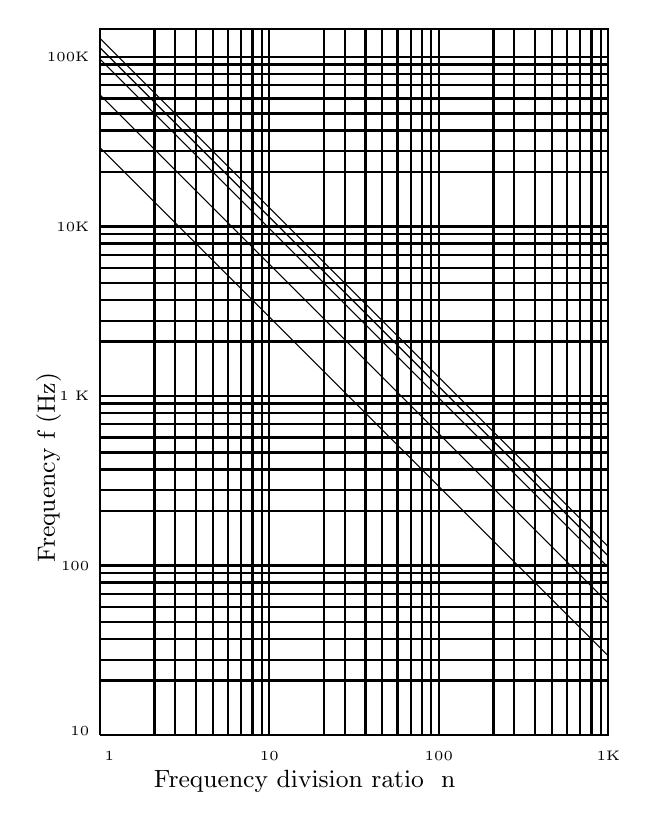
\begin{tikzpicture}
\tiny
\draw[thick] (0em,0em) -- (0em,37.5em) -- (27em,37.5em) -- (27em,0em) -- (0em,0em);

\draw[thick] (0em,2.9em) -- (27em,2.9em);
\draw[thick] (0em,4em) -- (27em,4em);
\draw[thick] (0em,5.1em) -- (27em,5.1em);
\draw[thick] (0em,6em) -- (27em,6em);
\draw[thick] (0em,6.8em) -- (27em,6.8em);
\draw[thick] (0em,7.5em) -- (27em,7.5em);
\draw[thick] (0em,8.1em) -- (27em,8.1em);
\draw[thick] (0em,8.6em) -- (27em,8.6em);
\draw[thick] (0em,9em) -- (27em,9em);

\draw[thick] (0em,11.9em) -- (27em,11.9em);
\draw[thick] (0em,13em) -- (27em,13em);
\draw[thick] (0em,14.1em) -- (27em,14.1em);
\draw[thick] (0em,15em) -- (27em,15em);
\draw[thick] (0em,15.8em) -- (27em,15.8em);
\draw[thick] (0em,16.5em) -- (27em,16.5em);
\draw[thick] (0em,17.1em) -- (27em,17.1em);
\draw[thick] (0em,17.6em) -- (27em,17.6em);
\draw[thick] (0em,18em) -- (27em,18em);

\draw[thick] (0em,20.9em) -- (27em,20.9em);
\draw[thick] (0em,22em) -- (27em,22em);
\draw[thick] (0em,23.1em) -- (27em,23.1em);
\draw[thick] (0em,24em) -- (27em,24em);
\draw[thick] (0em,24.8em) -- (27em,24.8em);
\draw[thick] (0em,25.5em) -- (27em,25.5em);
\draw[thick] (0em,26.1em) -- (27em,26.1em);
\draw[thick] (0em,26.6em) -- (27em,26.6em);
\draw[thick] (0em,27em) -- (27em,27em);

\draw[thick] (0em,29.9em) -- (27em,29.9em);
\draw[thick] (0em,31em) -- (27em,31em);
\draw[thick] (0em,32.1em) -- (27em,32.1em);
\draw[thick] (0em,33em) -- (27em,33em);
\draw[thick] (0em,33.8em) -- (27em,33.8em);
\draw[thick] (0em,34.5em) -- (27em,34.5em);
\draw[thick] (0em,35.1em) -- (27em,35.1em);
\draw[thick] (0em,35.6em) -- (27em,35.6em);
\draw[thick] (0em,36em) -- (27em,36em);

\draw[thick] (2.9em,0em) -- (2.9em,37.5em);
\draw[thick] (4em,0em) -- (4em,37.5em);
\draw[thick] (5.1em,0em) -- (5.1em,37.5em);
\draw[thick] (6em,0em) -- (6em,37.5em);
\draw[thick] (6.8em,0em) -- (6.8em,37.5em);
\draw[thick] (7.5em,0em) -- (7.5em,37.5em);
\draw[thick] (8.1em,0em) -- (8.1em,37.5em);
\draw[thick] (8.6em,0em) -- (8.6em,37.5em);
\draw[thick] (9em,0em) -- (9em,37.5em);

\draw[thick] (11.9em,0em) -- (11.9em,37.5em);
\draw[thick] (13em,0em) -- (13em,37.5em);
\draw[thick] (14.1em,0em) -- (14.1em,37.5em);
\draw[thick] (15em,0em) -- (15em,37.5em);
\draw[thick] (15.8em,0em) -- (15.8em,37.5em);
\draw[thick] (16.5em,0em) -- (16.5em,37.5em);
\draw[thick] (17.1em,0em) -- (17.1em,37.5em);
\draw[thick] (17.6em,0em) -- (17.6em,37.5em);
\draw[thick] (18em,0em) -- (18em,37.5em);

\draw[thick] (20.9em,0em) -- (20.9em,37.5em);
\draw[thick] (22em,0em) -- (22em,37.5em);
\draw[thick] (23.1em,0em) -- (23.1em,37.5em);
\draw[thick] (24em,0em) -- (24em,37.5em);
\draw[thick] (24.8em,0em) -- (24.8em,37.5em);
\draw[thick] (25.5em,0em) -- (25.5em,37.5em);
\draw[thick] (26.1em,0em) -- (26.1em,37.5em);
\draw[thick] (26.6em,0em) -- (26.6em,37.5em);
\draw[thick] (27em,0em) -- (27em,37.5em);

\draw (0em,37em) -- (27em,10em);
\draw (0em,36.5em) -- (27em,9.5em);
\draw (0em,35.9em) -- (27em,8.9em);
\draw (0em,34em) -- (27em,7em);
\draw (0em,31.2em) -- (27em,4.2em);

\draw (0.5em,-0.5em) node[anchor=north]{1};
\draw (9em,-0.5em) node[anchor=north]{10};
\draw (18em,-0.5em) node[anchor=north]{100};
\draw (27em,-0.5em) node[anchor=north]{1K};

\draw (-0.2em,0.2em) node[anchor=east] {10};
\draw (-0.2em,9em) node[anchor=east] {100};
\draw (-0.2em,18em) node[anchor=east] {1 K};
\draw (-0.2em,27em) node[anchor=east] {10K};
\draw (-0.2em,36em) node[anchor=east] {100K};

\small
\draw (8em,-1em) node[anchor=north]{Frequency division ratio \ n};
\draw (-2em,14.5em) node[anchor=east,rotate=90] {Frequency f (Hz)};
\end{tikzpicture}

\vspace{0.5em}

\hskip 31em Frequency division ratio with\par
\hskip 31em respect to the output frequency

\newpage

\phantomsection
\addcontentsline{toc}{subsubsection}{(3) Example of frequency setting}

\noindent \ (3) \ Example of frequency setting\par
Consider an example in which the basic clock frequency is 3.579545 MHz and the desired\\
frequency of 440 Hz is output from TONE 1. (corresponding to“A"on the musical scale)\\

\phantomsection
\addcontentsline{toc}{subsubsection}{a. Calculation of frequency division ratio n}

\noindent \ a. \ \ Calculation of frequency division ratio n\par
n = N/(32 x f)\par
\ \ = 3579545/(32 x 440)\par
\ ≒ 254.229\par
n is a 10-bit integer, hence the nearest integral value is 254.\\
\par
Consequently, the frequency actually output is\par
f = N/(32 x n)\par
\ \ = 3579545/(32 x 254)\par
\ ≒ 440.397 (Hz)\\
\par
Here, the pitch error △C is obtained according to the following equation.\par
△C =\{(f'- f)/f\}/(\hskip -0.2em $\sqrt[1 \, 2 \, 0 \, 0 \ ]{ \ 2}$-1)\par
\ \ \ ≒\{(440.397-440)/440\}/(\hskip -0.2em $\sqrt[1 \, 2 \, 0 \, 0 \ ]{ \ 2}$-1)\par
\ \ \ ≒(0.397/440)/0.000578 ≒ 1.56\par
f: True frequency \ f'\hskip -0.5em: Actual frequency \ \hskip -0.2em $\sqrt[1 \, 2 \, 0 \, 0 \ ]{ \ 2}$\\

\phantomsection
\addcontentsline{toc}{subsubsection}{b. Data sent to PSG}

\noindent \  \ b. \ Data sent to PSG\par
n = 254\par
\ \ = 0011111110B\\
\par
\hskip 2em 1st byte \hskip 17em 2nd byte

\vspace{0.5em}
\setlength{\arrayrulewidth}{0.1em}
\setlength{\tabcolsep}{0.5em}
\renewcommand{\arraystretch}{2}
\hskip 2em \begin{tabular}{|c|c|c|c|c|c|c|c|c|c|c|c|c|c|c|c|c|}
\cline{1-8}
\cline{10-17}
* & \multicolumn{3}{c|}{REG. ADDR.} & \multicolumn{4}{c|}{n \ } & \ \ \ \ \ \ \ \ \ & * & & \multicolumn{6}{c|}{n \ \ \ \ \ }\\
\cline{1-8}
\cline{10-17}
1 & R2 & R1 & R0 & F3 & F2 & F1 & F0 & & 0 & × & F9 & F8 & F7 & F6 & F5 & F4\\
\cline{1-8}
\cline{10-17}
\multicolumn{17}{c}{}\\[-3.6em]
\multicolumn{17}{c}{}\\
\cline{1-8}
\cline{10-17}
D7 & D6 & D5 & D4 & D3 & D2 & D1 & D0 & & D7 & D6 & D5 & D4 & D3 & D2 & D1 & D0\\
\cline{1-8}
\cline{10-17}
1 & 0 & 0 & 0 & 1 & 1 & 1 & 0 & & 0 & × & 0 & 0 & 1 & 1 & 1 & 1\\
\cline{1-8}
\cline{10-17}
\end{tabular}

\vspace{2em}

\phantomsection
\addcontentsline{toc}{subsubsection}{(4) Tone level setting}

\noindent \ (4) Tone level setting\par
The frequency set by the tone generator is sent to the level setting section where the volume\\
level is set. \ The level setting section is a programmable attenuator which enables the volume level\\
to be set in 16 steps from 0 dB to OFF according to a 4-bit attenuation value.\\
\par
\hskip 2.5em 1st byte only

\vspace{0.5em}
\setlength{\arrayrulewidth}{0.1em}
\setlength{\tabcolsep}{0.5em}
\renewcommand{\arraystretch}{2}
\hskip 2em \begin{tabular}{|c|c|c|c|c|c|c|c|c|c|c|c|l|c|}
\cline{1-8}
\cline{10-14}
D7 & D6 & D5 & D4 & D3 & D2 & D1 & D0 & \ \ \ \ \ \ \ & R2 & R1 & R0 & Control register allocation \ & HEX \ \\
\cline{1-8}
\cline{10-14}
\multicolumn{8}{c}{} & & 0 & 0 & 1 & Tone 1 attenuation & 9×\\[-3.6em]
\multicolumn{8}{c}{} & & & & & &\\
\cline{1-8}
* & \multicolumn{3}{c|}{REG. ADDR.} & \multicolumn{4}{l|}{ATT. DATA} & & & & & &\\[-1.2em]
\cline{10-14}
& \multicolumn{3}{c|}{} & \multicolumn{4}{l|}{} & & 0 & 1 & 1 & Tone 2 attenuation & B×\\[-3.6em]
& \multicolumn{3}{c|}{} & \multicolumn{4}{l|}{} & & & & & &\\
\cline{1-8}
1 & R2 & R1 & R0 & A3 & A2 & A1 & A0 & & & & & &\\[-1.2em]
\cline{10-14}
& & & & & & & & & 1 & 0 & 1 & Tone 3 attenuation & D×\\[-1.2em]
\cline{1-8}
\multicolumn{8}{c}{} & & & & & &\\
\cline{10-14}
\end{tabular}

\newpage

\hskip 2.5em Attenuation

\vspace{0.5em}
\setlength{\arrayrulewidth}{0.1em}
\setlength{\tabcolsep}{0.5em}
\renewcommand{\arraystretch}{2}
\hskip 2em \begin{tabular}{|c|r|c|c|c|r|c|}
\cline{1-3}
\cline{5-7}
[db] & \ A3 A2 A1 A0 & HEX \ & & [db] & \ A3 A2 A1 A0 & HEX \ \\
\cline{1-3}
\cline{5-7}
0 & \ 0 0 0 0 & ×0 & & 16 & \ 1 0 0 0 & ×8\\
\cline{1-3}
\cline{5-7}
2 & \ 0 0 0 1 & ×1 & & 18 & \ 1 0 0 1 & ×9\\
\cline{1-3}
\cline{5-7}
4 & \ 0 0 1 0 & ×2 & & 20 & \ 1 0 1 0 & ×A\\
\cline{1-3}
\cline{5-7}
6 & \ 0 0 1 1 & ×3 & & 22 & \ 1 0 1 1 & ×B\\
\cline{1-3}
\cline{5-7}
8 & \ 0 1 0 0 & ×4 & & 24 & \ 1 1 0 0 & ×C\\
\cline{1-3}
\cline{5-7}
10 & \ 0 1 0 1 & ×5 & & 26 & \ 1 1 0 1 & ×D\\
\cline{1-3}
\cline{5-7}
12 & \ 0 1 1 0 & ×6 & & 28 & \ 1 1 1 0 & ×E\\
\cline{1-3}
\cline{5-7}
14 & \ 0 1 1 1 & ×7 & & OFF \ & \ 1 1 1 1 & ×F\\
\cline{1-3}
\cline{5-7}
\end{tabular}

\vspace{2em}

\phantomsection
\addcontentsline{toc}{subsection}{[2] Noise generator}

\noindent [2] \ Noise generator\par
The noise generator consists of a noise generator circuit and a level setting section.\\
The source of the noise supplied from the noise generator circuit is a shift register with EX-OR\\
feedback. \ Each time the noise control register changes, the shift register is cleared.\\
\par
The shift clock of this shift register is determined by four modes that are in turn determined\\
by NF0 and NF1. \ If NF0 = NF1 = 0, for example, the shift clock becomes (N/32)/16.\\
In this case, if FB = 0, this shift clock will be frequency-divided by 16, resulting in synchronous\\
noise of a frequency of N/(32 x 16 x 16). \ If FB = 1, the shift register will be driven by this\\
shift clock with EX-OR feedback, resulting in the generation of white noise.\\

\phantomsection
\addcontentsline{toc}{subsubsection}{(1) Noise generator circuit control}

\noindent \ (1) Noise generator circuit control\\
\par
\hskip 2.5em 1st byte only

\vspace{0.5em}
\setlength{\arrayrulewidth}{0.1em}
\setlength{\tabcolsep}{0.5em}
\renewcommand{\arraystretch}{2}
\hskip 2em \begin{tabular}{|c|c|c|c|c|c|r|r|l|c|l}
\cline{1-8}
D7 & D6 & D5 & D4 & D3 & D2 & \ \ D1 & \ \ D0 & \multicolumn{3}{c}{}\\
\cline{1-8}
\multicolumn{11}{c}{}\\[-3.6em]
\multicolumn{11}{c}{}\\
\cline{1-8}
*& \multicolumn{3}{c|}{REG. ADDR.} & & & \multicolumn{2}{l|}{SHIFT} & \multicolumn{3}{c}{}\\
\cline{1-8}
1 & 1 & 1 & 0 & × & FB & NF1 & NF0 & \multicolumn{3}{c}{}\\
\cline{1-8}
\multicolumn{11}{c}{}\\
\cline{1-5}
\cline{7-10}
& & & & & & & & & &\\[-3em]
FB & \multicolumn{4}{l|}{Noise} & & NF1 & NF0 & Shift clock \ \ \ \ \ \ \ \ & k &\\[-1.8em]
& \multicolumn{4}{r|}{Generation \ } & & & & & &\\[-0.5em]
\cline{1-5}
\cline{7-10}
0 & \multicolumn{4}{l|}{Synchronous} & & 0 & 0 & (N/32)/k & 16 & N:Basic clock\\[-1.2em]
& \multicolumn{4}{r|}{Noise \ \ } & & & & & &\\[-1.2em]
\cline{7-10}
& \multicolumn{4}{l|}{} & & 0 & 1 & (N/32)/k & 32 &\\[-1.2em]
\cline{1-5}
1 & \multicolumn{4}{r|}{White noise \ \ \ } & & & & & &\\[-1.2em]
\cline{7-10}
& \multicolumn{4}{l|}{} & & 1 & 0 & (N/32)/k & 64 &\\
\cline{1-5}
\cline{7-10}
\multicolumn{5}{c}{} & & 1 & 1 & Tone generator 3 & \multicolumn{2}{l}{←At this time, the tone of the}\\[-1.2em]
\multicolumn{5}{c}{} & & & & & \multicolumn{2}{l}{noise can be varied continuously}\\[-1.2em]
\cline{7-9}
\end{tabular}

\newpage

\phantomsection
\addcontentsline{toc}{subsubsection}{a. Synchronous noise (FB = 0)}

\noindent a. Synchronous noise (FB = 0)\\
\phantom \ When NF0 = NF1 = Value other than 1

\vspace{2em}
\setlength{\arrayrulewidth}{0.1em}
\setlength{\tabcolsep}{0.5em}
\renewcommand{\arraystretch}{2}
\hskip 3em \begin{tabular}{lc|c|c|c|c|ccc|c|c}
\cline{2-2}
\cline{4-4}
\cline{6-6}
\cline{10-10}
N/(32×k) & \ \ & \ \ \ \ \ \ \ & \ \ \ \ \ \ \ & \ \ \ \ \ \ \ & \ \ \ \ \ \ \ & \ \ \ \ \ \ \ & \ \ \ \ \ \ \ & \ \ \ \ \ \ \ & \ \ \ \ \ \ \ & \ \ \ \\
\cline{3-3}
\cline{5-5}
\cline{7-7}
\cdashline{8-8}[2.5pt/2.5pt]
\cline{9-9}
\cline{11-11}
\multicolumn{3}{c}{} & \multicolumn{2}{c}{1 clock \ } & \multicolumn{6}{c}{}\\[-3.6em]
\multicolumn{3}{c}{} & \multicolumn{2}{c}{} & \multicolumn{6}{c}{}\\
\multicolumn{3}{c|}{} & \multicolumn{2}{c|}{} & \multicolumn{4}{c|}{} & \multicolumn{2}{c}{}\\[-2.4em]
\multicolumn{3}{c|}{} & \multicolumn{2}{l|}{← \ \ pulse \ →} & \multicolumn{4}{l|}{← \ \ \ 15 clock pulses \ \ \ \ \ \ →} & \multicolumn{2}{c}{}\\[-1.2em]
\multicolumn{11}{c}{}\\[-3.6em]
\multicolumn{11}{c}{}\\
\cline{4-5}
\cline{10-11}
Noise & \multicolumn{2}{c|}{} & \multicolumn{2}{c|}{} & \multicolumn{4}{c|}{} & \multicolumn{2}{c}{}\\
\cline{2-3}
\cline{6-7}
\cdashline{8-8}[2.5pt/2.5pt]
\cline{9-9}
\end{tabular}

\vspace{2em}
\noindent {*} The noise frequency is (N/(32 x k))/16 = N/(32 x k x 16)\\
\\
\phantom \ When NF0 = NF1 = 1 (Control by tone 3)

\vspace{2em}
\setlength{\arrayrulewidth}{0.1em}
\setlength{\tabcolsep}{0.5em}
\renewcommand{\arraystretch}{2}
\hskip 3em \begin{tabular}{lc|c|c|c|c|ccc|c|c}
\cline{2-2}
\cline{4-4}
\cline{6-6}
\cline{10-10}
Tone 3 \ \ \ \ \ \ \ \ \ & \ \ & \ \ \ \ \ \ \ & \ \ \ \ \ \ \ & \ \ \ \ \ \ \ & \ \ \ \ \ \ \ & \ \ \ \ \ \ \ & \ \ \ \ \ \ \ & \ \ \ \ \ \ \ & \ \ \ \ \ \ \ & \ \ \ \\
\cline{3-3}
\cline{5-5}
\cline{7-7}
\cdashline{8-8}[2.5pt/2.5pt]
\cline{9-9}
\cline{11-11}
\multicolumn{3}{c}{} & \multicolumn{2}{c}{1 clock \ } & \multicolumn{6}{c}{}\\[-3.6em]
\multicolumn{3}{c}{} & \multicolumn{2}{c}{} & \multicolumn{6}{c}{}\\
\multicolumn{3}{c|}{} & \multicolumn{2}{c|}{} & \multicolumn{4}{c|}{} & \multicolumn{2}{c}{}\\[-2.4em]
\multicolumn{3}{c|}{} & \multicolumn{2}{l|}{← \ pulse \ \ →} & \multicolumn{4}{l|}{← \ \ \ 15 clock pulses \ \ \ \ \ \ →} & \multicolumn{2}{c}{}\\[-1.2em]
\multicolumn{11}{c}{}\\[-3.6em]
\multicolumn{11}{c}{}\\
\cline{4-5}
\cline{10-11}
Noise & \multicolumn{2}{c|}{} & \multicolumn{2}{c|}{} & \multicolumn{4}{c|}{} & \multicolumn{2}{c}{}\\
\cline{2-3}
\cline{6-7}
\cdashline{8-8}[2.5pt/2.5pt]
\cline{9-9}
\end{tabular}

\vspace{2em}
\noindent {*} The noise frequency is (frequency TONE 3)/16 = N/(32 x n x 16)\\

\phantomsection
\addcontentsline{toc}{subsubsection}{b. White Noise (FB = 1)}

\noindent b. White Noise (FB = 1)\par
Spectrum when NF0 = 0 NF1 = 1 n=1\\

\hskip -1em 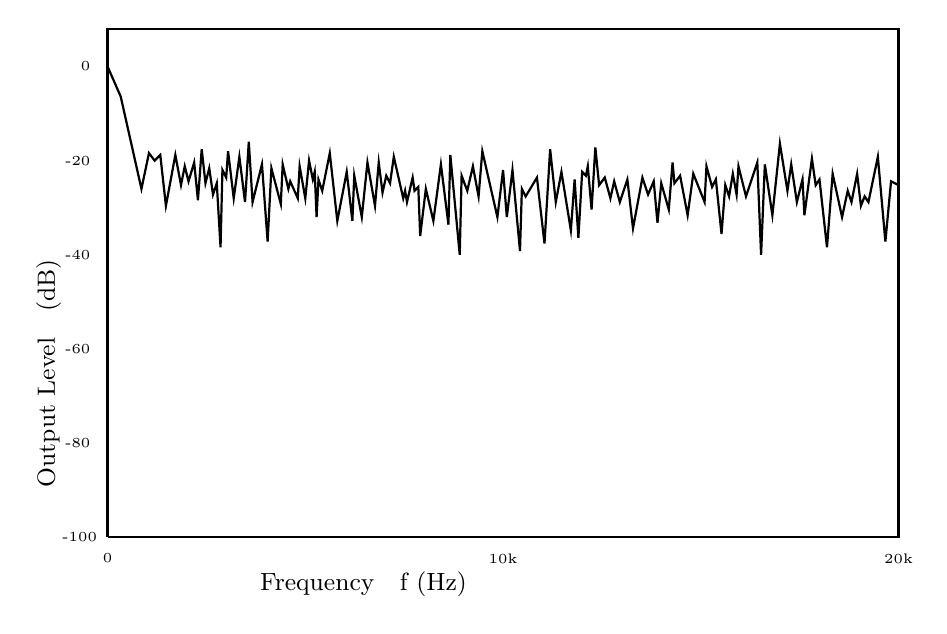
\begin{tikzpicture}
\tiny
\draw[thick] (0em,0em) -- (0em,27em) -- (42em,27em) -- (42em,0em) -- (0em,0em);

\draw (0em,-0.5em) node[anchor=north]{0};
\draw (21em,-0.5em) node[anchor=north]{10k};
\draw (42em,-0.5em) node[anchor=north]{20k};

\draw (-0.2em,0em) node[anchor=east] {-100};
\draw (-0.2em,5em) node[anchor=east] {-80 \ };
\draw (-0.2em,10em) node[anchor=east] {-60 \ };
\draw (-0.2em,15em) node[anchor=east] {-40 \ };
\draw (-0.2em,20em) node[anchor=east] {-20 \ };
\draw (-0.2em,25em) node[anchor=east] {0 \ };

\draw[thick] (0em,25em) -- (0.7em,23.4em) -- (1.8em,18.5em) -- (2.2em,20.4em) -- (2.5em,20em) -- (2.8em,20.3em) -- (3.1em,17.6em) -- (3.6em,20.3em) -- (3.9em,18.7em) -- (4.1em,19.7em) -- (4.3em,18.9em) -- (4.6em,19.9em) -- (4.8em,17.9em) -- (5em,20.6em) -- (5.2em,18.8em) -- (5.4em,19.6em)  -- (5.6em,18.2em) -- (5.8em,18.8em) -- (6em,15.4em) -- (6.1em,19.5em) -- (6.3em,19.1em) -- (6.4em,20.5em) -- (6.7em,18em) -- (7em,20.2em) -- (7.3em,17.8em) -- (7.5em,21em) -- (7.7em,17.8em) -- (8.2em,19.8em) -- (8.5em,15.7em) -- (8.7em,19.6em) -- (9.2em,17.7em) -- (9.3em,19.8em) -- (9.6em,18.5em) -- (9.7em,18.9em) -- (10.1em,18em) -- (10.2em,19.7em) -- (10.5em,18em) -- (10.7em,20em) -- (10.9em,19em) -- (11em,19.4em) -- (11.1em,17em) -- (11.2em,19em) -- (11.4em,18.4em) -- (11.8em,20.4em) -- (12.2em,16.8em) -- (12.7em,19.4em) -- (13em,16.8em) -- (13.1em,19.2em) -- (13.5em,17em) -- (13.8em,19.9em) -- (14.2em,17.6em) -- (14.4em,19.9em) -- (14.6em,18.3em) -- (14.8em,19.2em) -- (15em,18.8em) -- (15.2em,20.2em) -- (15.7em,18em) -- (15.8em,18.4em) -- (15.9em,17.8em) -- (16.2em,19.1em) -- (16.3em,18.4em) -- (16.5em,18.6em) -- (16.6em,16em) -- (16.9em,18.5em) -- (17.3em,16.8em) -- (17.7em,19.8em) -- (18.1em,16.6em) -- (18.2em,20.3em) -- (18.7em,15em) -- (18.8em,19.2em) -- (19.1em,18.4em) -- (19.4em,19.7em) -- (19.7em,18.1em) -- (19.9em,20.5em) -- (20.7em,17em) -- (21em,19.5em) -- (21.2em,17em) -- (21.5em,19.5em) -- (21.9em,15.2em) -- (22em,18.5em) -- (22.2em,18.1em) -- (22.8em,19.1em) -- (23.2em,15.6em) -- (23.5em,20.6em) -- (23.8em,17.8em) -- (24.1em,19.4em) -- (24.6em,16.3em) -- (24.8em,19em) -- (25em,15.9em) -- (25.2em,19.4em) -- (25.4em,19.2em) -- (25.5em,19.7em) -- (25.7em,17.4em) -- (25.9em,20.7em) -- (26.1em,18.7em) -- (26.4em,19.1em) -- (26.7em,18em) -- (26.9em,18.9em) -- (27.2em,17.8em) -- (27.6em,19em) -- (27.9em,16.4em) -- (28.4em,19.1em) -- (28.7em,18.2em) -- (29em,18.9em) -- (29.2em,16.7em) -- (29.4em,18.8em) -- (29.8em,17.4em) -- (30em,19.9em) -- (30.1em,18.8em) -- (30.4em,19.2em) -- (30.8em,17.1em) -- (31.1em,19.3em) -- (31.7em,17.8em) -- (31.8em,19.7em) -- (32.1em,18.6em) -- (32.3em,19em) -- (32.6em,16.1em) -- (32.8em,18.7em) -- (33em,18.1em) -- (33.2em,19.3em) -- (33.4em,18.2em) -- (33.5em,19.7em) -- (33.9em,18.1em) -- (34.5em,19.9em) -- (34.7em,15em) -- (34.9em,19.8em) -- (35.3em,17.1em) -- (35.7em,20.9em) -- (36.1em,18.4em) -- (36.3em,19.8em) -- (36.6em,17.8em) -- (36.9em,19em) -- (37em,17.1em) -- (37.4em,20.1em) -- (37.6em,18.7em) -- (37.8em,19em) -- (38.2em,15.4em) -- (38.5em,19.3em) -- (39em,17em) -- (39.3em,18.4em) -- (39.5em,17.8em) -- (39.8em,19.3em) -- (40em,17.6em) -- (40.2em,18.1em) -- (40.4em,17.8em) -- (40.9em,20.2em) -- (41.3em,15.7em) -- (41.6em,18.9em) -- (42em,18.7em);

\small
\draw (10em,-1em) node[anchor=north]{Frequency \ \ f (Hz)};
\draw (-2.3em,11.2em) node[anchor=east,rotate=90] {Output Level \ \ (dB)};
\end{tikzpicture}

\vspace{1.5em}

\phantomsection
\addcontentsline{toc}{subsubsection}{(2) Noise level setting}

\noindent \ (2) Noise level setting\par
\hskip 2em 1st byte only

\vspace{0.5em}
\setlength{\arrayrulewidth}{0.1em}
\setlength{\tabcolsep}{0.5em}
\renewcommand{\arraystretch}{2}
\hskip 2em \begin{tabular}{|c|c|c|c|c|c|c|c|}
\cline{1-8}
D7 & D6 & D5 & D4 & D3 & D2 & D1 & D0\\
\cline{1-8}
\multicolumn{8}{c}{}\\[-3.6em]
\multicolumn{8}{c}{}\\
\cline{1-8}
*& \multicolumn{3}{c|}{REG. ADDR.} & \multicolumn{4}{l|}{ATT. DATA}\\
\cline{1-8}
1 & 1 & 1 & 1 & A3 & A2 & A1 & A0\\
\cline{1-8}
\end{tabular}

\vspace{2em}
\noindent {*} The attenuation control is the same as for“Tone"\hskip -0.5em.

\newpage

\phantomsection
\addcontentsline{toc}{subsection}{[3] Register address feed}

\noindent [3] \ Register address feed\par
PSG uses the three bits R2 to R0 of the 1st byte to judge which control register the data has\\
been sent from.

\vspace{0.5em}
\setlength{\arrayrulewidth}{0.1em}
\setlength{\tabcolsep}{0.5em}
\renewcommand{\arraystretch}{2}
\hskip 2em \begin{tabular}{|c|c|c|l|c|}
\cline{1-5}
R2 & R1 & R0 & Control register allocation \ \ \ \ \ & \ 1st \ \\
\cline{1-5}
0 & 0 & 0 & Tone 1 frequency division ratio & 8×\\
\cline{1-5}
0 & 0 & 1 & Tone 1 attenuation & 9×\\
\cline{1-5}
0 & 1 & 0 & Tone 2 frequency division ratio & A×\\
\cline{1-5}
0 & 1 & 1 & Tone 2 attenuation & B×\\
\cline{1-5}
1 & 0 & 0 & Tone 3 frequency division ratio & C×\\
\cline{1-5}
1 & 0 & 1 & Tone 3 attenuation & D×\\
\cline{1-5}
1 & 1 & 0 & Noise generator circuit control & E×\\
\cline{1-5}
1 & 1 & 1 & Noise attenuation & F×\\
\cline{1-5}
\end{tabular}

\vspace{2em}

\phantomsection
\addcontentsline{toc}{subsection}{[4] Correlation between the sound elements and PSG}

\noindent [4] \ Correlation between the sound elements and PSG

\vspace{2em}
\setlength{\arrayrulewidth}{0.1em}
\setlength{\tabcolsep}{0.5em}
\renewcommand{\arraystretch}{2}
\hskip -2em \begin{tabular}{|l|l|l|}
\cline{1-3}
Sound element \ & Physical element & \ \ Correlation with PSG\\
\cline{1-3}
Pitch of sound & \ Frequency & \ [1] - (2) Tone frequency setting,\\[-1.2em]
& & \ [2] - (1) Noise generator circuit control\\
\cline{1-3}
Tone & \ Harmonic & This is mainly related to wave length. \ In the tone generation\\[-1.2em]
& \ \ \ \ components & mode, the PSG can output three frequencies simultaneously from\\[-1.2em]
& & only a 50\% duty pulse waveform. Consequently, by combining\\[-1.2em]
& & attenuation control with this mode, the harmonic components\\[-1.2em]
& & can be controlled. In the synchronous noise mode, a 6.25\%\\[-1.2em]
& & duty pulse waveform.\\
\cline{1-3}
Strength & \ Amplitude & As described in [1] - (3) and [2] - (2), the attenuation of\\[-1.2em]
\ \ \ \ \ \ of tone & & the three tones and noise can be controlled by 4-bit data.\\
\cline{1-3}
Way & \ Envelope & The wave length at left can be realized by using external data\\[-1.2em]
in which sound & & to control each attenuation. \ This can be done in the range\\[-1.2em]
is emitted. & & where the 4-bit attenuation data is rewritten and envelope\\[-1.2em]
& & sequence control performed at each step. The tone and noise\\[-1.2em]
& & frequencies can be controlled by the range in which component\\[-1.2em]
& & control can be performed.\\
\cline{1-3}
\end{tabular}

\vspace{-4.8em}

\hskip 6.8em 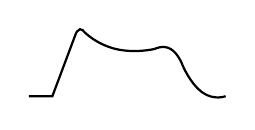
\begin{tikzpicture}
\draw [thick]  (0,0) -- (0.3,0) -- (0.6,0.8);
\draw [thick] plot [smooth, tension=1] coordinates {(0.6,0.8) (0.65,0.85) (0.7,0.82)};
\draw [thick] plot [smooth, tension=1] coordinates {(0.7,0.82) (1.1,0.6) (1.6,0.6)};
\draw [thick] plot [smooth, tension=1] coordinates {(1.6,0.6) (1.8,0.6) (1.95,0.4)};
\draw [thick] plot [smooth, tension=1] coordinates {(1.95,0.4) (2.2,0.05) (2.5,0.0)};
\end{tikzpicture}

\vspace{8em}

\phantomsection
\addcontentsline{toc}{subsubsection}{Relation between musical interval and frequency division ratio}

\noindent (next page)\\
Relation between musical interval and frequency division ratio for scale divided equally into 12\\
parts (basic clock: 3.579545 MHz)

\newpage

\vspace{0.5em}
\setlength{\arrayrulewidth}{0.1em}
\setlength{\tabcolsep}{0.5em}
\renewcommand{\arraystretch}{2}
\hskip 2em \begin{tabular}{|r|r|c|c|r|r|}
\cline{1-6}
Musical \ \ \ & Frequency \ \ \ & \multicolumn{2}{c|}{\ \ \ \ \ \ HEX \ \ \ \ \ \ } & \ \ \ \ \ \ \ \ \ \ \ \ \ \ \ \ \ \ \ \ \ & \ \ \ \ \ \ \ \ \ \ \ \ \ \ \ \ \ \ \ \ \ \\[-1.2em]
interval \ & division \ \ & \multicolumn{2}{c|}{} & PSG output \ \ \ \ \ & Actual frequency \ \ \\[-3.6em]
& & \multicolumn{2}{c|}{} & &\\
\cline{3-4}
& ratio \ \ \ \ \ & \ \ 1st \ \ & 2nd & [Hz] \ \ \ \ \ \ \ \ & [Hz] \ \ \ \ \ \ \ \ \\
\cline{1-6}
\ A 2 \ \ & 1017 \ \ & X9 & 3F & 109.991 \ \ & 110.000 \ \ \\[-1.2em]
\ A\hskip 0.1em $^\#$2 \ \ & 960 \ \ & X0 & 3C & 116.522 \ \ & 116.541 \ \ \\[-1.2em]
\ B 2 \ \ & 906 \ \ & XA & 38 & 123.467 \ \ & 123.471 \ \ \\[-1.2em]
\ C 3 \ \ & 855 \ \ & X7 & 35 & 130.832 \ \ & 130.813 \ \ \\[-1.2em]
\ C\hskip 0.1em $^\#$3 \ \ & 807 \ \ & X7 & 32 & 138.613 \ \ & 138.591 \ \ \\[-1.2em]
\ D 3 \ \ & 762 \ \ & XA & 2F & 146.799 \ \ & 146.832 \ \ \\[-1.2em]
\ D\hskip 0.1em $^\#$3 \ \ & 719 \ \ & XF & 2C & 155.578 \ \ & 155.563 \ \ \\[-1.2em]
\ E 3 \ \ & 679 \ \ & X7 & 2A & 164.744 \ \ & 164.814 \ \ \\[-1.2em]
\ F 3 \ \ & 641 \ \ & X1 & 28 & 174.510 \ \ & 174.614 \ \ \\[-1.2em]
\ F\hskip 0.1em $^\#$3 \ \ & 605 \ \ & XD & 25 & 184.894 \ \ & 184.997 \ \ \\[-1.2em]
\ G 3 \ \ & 571 \ \ & XB & 23 & 195.904 \ \ & 195.998 \ \ \\[-1.2em]
\ G\hskip 0.1em $^\#$3 \ \ & 539 \ \ & XB & 21 & 207.534 \ \ & 207.652 \ \ \\[-1.2em]
\ A 3 \ \ & 508 \ \ & XC & 1F & 220.199 \ \ & 220.000 \ \ \\[-1.2em]
\ A\hskip 0.1em $^\#$3 \ \ & 480 \ \ & X0 & 1E & 233.044 \ \ & 233.082 \ \ \\[-1.2em]
\ B 3 \ \ & 453 \ \ & X5 & 1C & 246.934 \ \ & 246.942 \ \ \\[-1.2em]
\ C 4 \ \ & 428 \ \ & XC & 1A & 261.357 \ \ & 261.626 \ \ \\[-1.2em]
\ C\hskip 0.1em $^\#$4 \ \ & 404 \ \ & X4 & 19 & 276.884 \ \ & 277.183 \ \ \\[-1.2em]
\ D 4 \ \ & 381 \ \ & XD & 17 & 293.598 \ \ & 293.665 \ \ \\[-1.2em]
\ D\hskip 0.1em $^\#$4 \ \ & 360 \ \ & X8 & 16 & 310.725 \ \ & 311.127 \ \ \\[-1.2em]
\ E 4 \ \ & 339 \ \ & X3 & 15 & 329.973 \ \ & 329.628 \ \ \\[-1.2em]
\ F 4 \ \ & 320 \ \ & X0 & 14 & 349.565 \ \ & 349.228 \ \ \\[-1.2em]
\ F\hskip 0.1em $^\#$4 \ \ & 302 \ \ & XE & 12 & 370.400 \ \ & 369.994 \ \ \\[-1.2em]
\ G 4 \ \ & 285 \ \ & XD & 11 & 392.495 \ \ & 391.995 \ \ \\[-1.2em]
\ G\hskip 0.1em $^\#$4 \ \ & 269 \ \ & XD & 10 & 415.840 \ \ & 415.305 \ \ \\[-1.2em]
\ A 4 \ \ & 254 \ \ & XE & 0F & 440.397 \ \ & 440.000 \ \ \\[-1.2em]
\ A\hskip 0.1em $^\#$4 \ \ & 240 \ \ & X0 & 0F & 466.087 \ \ & 466.164 \ \ \\[-1.2em]
\ B 4 \ \ & 226 \ \ & X2 & 0E & 494.960 \ \ & 493.883 \ \ \\[-1.2em]
\ C 5 \ \ & 214 \ \ & X6 & 0D & 522.715 \ \ & 523.251 \ \ \\[-1.2em]
\ C\hskip 0.1em $^\#$5 \ \ & 202 \ \ & XA & 0C & 553.767 \ \ & 554.365 \ \ \\[-1.2em]
\ D 5 \ \ & 190 \ \ & XE & 0B & 588.742 \ \ & 587.330 \ \ \\[-1.2em]
\ D\hskip 0.1em $^\#$5 \ \ & 180 \ \ & X4 & 0B & 621.450 \ \ & 622.254 \ \ \\[-1.2em]
\ E 5 \ \ & 170 \ \ & XA & 0A & 658.005 \ \ & 659.255 \ \ \\[-1.2em]
\ F 5 \ \ & 160 \ \ & X0 & 0A & 699.131 \ \ & 698.456 \ \ \\[-1.2em]
\ F\hskip 0.1em $^\#$5 \ \ & 151 \ \ & X7 & 09 & 740.801 \ \ & 739.989 \ \ \\[-1.2em]
\ G 5 \ \ & 143 \ \ & XF & 08 & 782.244 \ \ & 783.991 \ \ \\[-1.2em]
\ G\hskip 0.1em $^\#$5 \ \ & 135 \ \ & X7 & 08 & 828.600 \ \ & 830.609 \ \ \\[-1.2em]
\ A 5 \ \ & 127 \ \ & XF & 07 & 880.795 \ \ & 880.000 \ \ \\[-1.2em]
\ A\hskip 0.1em $^\#$5 \ \ & 120 \ \ & X8 & 07 & 932.174 \ \ & 932.328 \ \ \\[-1.2em]
\ B 5 \ \ & 113 \ \ & X1 & 07 & 989.920 \ \ & 987.767 \ \ \\[-1.2em]
\ C 6 \ \ & 107 \ \ & XB & 06 & 1045.429 \ \ & 1046.502 \ \ \\[-1.2em]
\ C\hskip 0.1em $^\#$6 \ \ & 101 \ \ & X5 & 06 & 1107.534 \ \ & 1108.731 \ \ \\[-1.2em]
\ D 6 \ \ & 95 \ \ & XF & 05 & 1177.484 \ \ & 1174.659 \ \ \\[-1.2em]
\ D\hskip 0.1em $^\#$6 \ \ & 90 \ \ & XA & 05 & 1242.899 \ \ & 1244.508 \ \ \\[-1.2em]
\ E 6 \ \ & 85 \ \ & X5 & 05 & 1316.011 \ \ & 1318.510 \ \ \\[-1.2em]
\ F 6 \ \ & 80 \ \ & X0 & 05 & 1398.262 \ \ & 1396.913 \ \ \\[-1.2em]
\ F\hskip 0.1em $^\#$6 \ \ & 76 \ \ & XC & 04 & 1471.854 \ \ & 1479.978 \ \ \\[-1.2em]
\ G 6 \ \ & 71 \ \ & X7 & 04 & 1575.506 \ \ & 1567.982 \ \ \\[-1.2em]
\ G\hskip 0.1em $^\#$6 \ \ & 67 \ \ & X3 & 04 & 1669.566 \ \ & 1661.219 \ \ \\[-1.2em]
\ A 6 \ \ & 64 \ \ & X0 & 04 & 1747.827 \ \ & 1760.000 \ \ \\[-1.2em]
\ A\hskip 0.1em $^\#$6 \ \ & 60 \ \ & XC & 03 & 1864.349 \ \ & 1864.655 \ \ \\[-1.2em]
\ B 6 \ \ & 57 \ \ & X9 & 03 & 1962.473 \ \ & 1975.533 \ \ \\
\cline{1-6}
\end{tabular}

\newpage

\noindent {*} f = 3579545/(32 x n) \ n: 10-bit frequency division \ \ Maximum frequency is n = 1\\
\phantom \ {*} In the previous table, musical interval was calculated on the basis of 440 Hz as concert pitch.\\
\phantom \ {*} Regarding HEX, the X part is as follows:\\
\\
\phantom \ \ Tone 1 → \ 8\\
\phantom \ \ Tone 2 → \ A\\
\phantom \ \ Tone 3 → \ C\\
\phantom \ 1st is the 1st byte\\
\phantom \ 2nd is the 2nd byte\\
\\
The upper limit is 3579545/32$\cdotp$1\\
\par
\hskip 21.5em TONE 1 to 3\par
\hskip 21.5em Duty 50\%\\[8em]
\par
\hskip 21.5em Base tone in synchronous noise mode\par
\hskip 21.5em Duty 6.25\%

\vspace{-14em}
\setlength{\arrayrulewidth}{0.1em}
\setlength{\tabcolsep}{0.5em}
\renewcommand{\arraystretch}{2}
\hskip -3.5em \begin{tabular}{cccl}
\cline{1-3}
\ \ \ \ \ \ \ & \ \ \ \ \ \ & \ \ \ \ \ \ \ &\\[-1.5em]
\cline{1-3}
& ○ & & \footnotesize{ \ ← \ \ 440\ \ \ Hz \ \ A\,$_4$}\\[-1.6em]
\cline{1-3}
& & &\\[-1.5em]
\cline{1-3}
& & &\\[-1.5em]
\cline{1-3}
& & &\\[-1.5em]
\cline{2-2}
& & &\\[-2.8em]
& ○ & & \footnotesize{ \ ← \ \ 220\ \ \ Hz \ \ A\,$_3$}\\[-1.1em]
\cline{1-3}
& & &\\[-1.5em]
\cline{1-3}
& & &\\[-1.5em]
\cline{1-3}
& ○ & & \footnotesize{ \ ← \ \ 110\ \ \ Hz \ \ A\,$_2$}\\[-1.6em]
\cline{1-3}
& & &\\[-1.5em]
\cline{1-3}
& & &\\[-1.5em]
\cline{2-2}
& & &\\[-1.5em]
\cline{2-2}
& & &\\[-2.8em]
& ○ & & \footnotesize{ \ ← \ \ \ 55\ \ \ Hz \ \ A\,$_1$}\\[-1.1em]
\cline{2-2}
& & &\\[-1.5em]
\cline{2-2}
& & &\\[-1.5em]
\cline{2-2}
& ○ & & \footnotesize{ \ ← \ \ \ 27.5 Hz \ \ A\,$_0$}\\[-1.6em]
\cline{2-2}
& & &\\[-1.5em]
\cline{2-2}
& & &\\[-1.5em]
\cline{2-2}
& & &\\[-1.5em]
\cline{2-2}
& & &\\[-2.8em]
& ○ & & \footnotesize{ \ ← \ \ \ 13.75Hz}\\[-1.1em]
\cline{2-2}
& & &\\[-1.5em]
\cline{2-2}
\end{tabular}

\vspace{-24em}

\[
\left.
\hskip -9.5em \begin{tabular}{c}
\\[11em]
\end{tabular}
\right \}
\] 

\[
\left.
\hskip -9.5em \begin{tabular}{c}
\\[5em]
\end{tabular}
\right \}
\] 

\begin{picture}(0,0)
\put(-28,149){
\includegraphics[width=1.9em]{TrebleClef}}
\put(-24,108){
\includegraphics[width=2.6em]{BassClef}}
\end{picture}

\newpage

\phantomsection
\addcontentsline{toc}{subsubsection}{Synchronous noise mode}

If a frequency of no greater than that generated by the tone generator is output, the outputs\\
shown in the table below will be obtained due to the synchronous noise mode of the noise generator\\
section. \ (Basic clock: 3.579545 MHz)

\vspace{2em}
\setlength{\arrayrulewidth}{0.1em}
\setlength{\tabcolsep}{0.5em}
\renewcommand{\arraystretch}{2}
\hskip 2em \begin{tabular}{|r|r|c|c|r|r|}
\cline{1-6}
Musical \ \ \ & Frequency \ \ \ & \multicolumn{2}{c|}{\ \ HEX (TONE3) \ \ } & \ \ \ \ \ \ \ \ \ \ \ \ \ \ \ \ \ \ \ \ \ & \ \ \ \ \ \ \ \ \ \ \ \ \ \ \ \ \ \ \ \ \ \\[-1.2em]
interval \ & division \ \ \ \  & \multicolumn{2}{c|}{} & PSG output \ \ \ \ \ & Actual frequency \ \ \\[-3.6em]
& & \multicolumn{2}{c|}{} & &\\
\cline{3-4}
& ratio \ \ \ \ \ \ \ & \ \ 1st \ \ & 2nd & [Hz] \ \ \ \ \ \ \ \ & [Hz] \ \ \ \ \ \ \ \ \\
\cline{1-6}
\ C 0 \ \ & 428 \ \ & CC & 1A & 16.335 \ \ & 16.352 \ \ \\[-1.2em]
\ C\hskip 0.1em $^\#$0 \ \ & 404 \ \ & C4 & 19 & 17.305 \ \ & 17.324 \ \ \\[-1.2em]
\ D 0 \ \ & 381 \ \ & CD & 17 & 18.350 \ \ & 18.354 \ \ \\[-1.2em]
\ D\hskip 0.1em $^\#$0 \ \ & 360 \ \ & C8 & 16 & 19.420 \ \ & 19.445 \ \ \\[-1.2em]
\ E 0 \ \ & 339 \ \ & C3 & 15 & 20.623 \ \ & 20.602 \ \ \\[-1.2em]
\ F 0 \ \ & 320 \ \ & C0 & 14 & 21.848 \ \ & 21.827 \ \ \\[-1.2em]
\ F\hskip 0.1em $^\#$0 \ \ & 302 \ \ & CE & 12 & 23.150 \ \ & 23.125 \ \ \\[-1.2em]
\ G 0 \ \ & 285 \ \ & CD & 11 & 24.531 \ \ & 24.500 \ \ \\[-1.2em]
\ G\hskip 0.1em $^\#$0 \ \ & 269 \ \ & CD & 10 & 25.990 \ \ & 25.957 \ \ \\[-1.2em]
\ A 0 \ \ & 254 \ \ & CE & 0F & 27.525 \ \ & 27.500 \ \ \\[-1.2em]
\ A\hskip 0.1em $^\#$0 \ \ & 240 \ \ & C0 & 0F & 29.130 \ \ & 29.135 \ \ \\[-1.2em]
\ B 0 \ \ & 226 \ \ & C2 & 0E & 30.935 \ \ & 30.868 \ \ \\[-1.2em]
\ C 1 \ \ & 214 \ \ & C6 & 0D & 32.670 \ \ & 32.703 \ \ \\[-1.2em]
\ C\hskip 0.1em $^\#$1 \ \ & 202 \ \ & CA & 0C & 34.610 \ \ & 34.648 \ \ \\[-1.2em]
\ D 1 \ \ & 190 \ \ & CE & 0B & 36.796 \ \ & 36.708 \ \ \\[-1.2em]
\ D\hskip 0.1em $^ \#$1 \ \ & 180 \ \ & C4 & 0B & 38.841 \ \ & 38.891 \ \ \\[-1.2em]
\ E 1 \ \ & 170 \ \ & CA & 0A & 41.125 \ \ & 41.203 \ \ \\[-1.2em]
\ F 1 \ \ & 160 \ \ & C0 & 0A & 43.696 \ \ & 43.654 \ \ \\[-1.2em]
\ F\hskip 0.1em $^ \#$1 \ \ & 151 \ \ & C7 & 09 & 46.300 \ \ & 46.249 \ \ \\[-1.2em]
\ G 1 \ \ & 143 \ \ & CF & 08 & 48.890 \ \ & 48.999 \ \ \\[-1.2em]
\ G\hskip 0.1em $^ \#$1 \ \ & 135 \ \ & C7 & 08 & 51.787 \ \ & 51.913 \ \ \\[-1.2em]
\ A 1 \ \ & 127 \ \ & CF & 07 & 55.050 \ \ & 55.000 \ \ \\[-1.2em]
\ A\hskip 0.1em $^ \#$1 \ \ & 120 \ \ & C8 & 07 & 58.261 \ \ & 58.270 \ \ \\[-1.2em]
\ B 1 \ \ & 113 \ \ & C1 & 07 & 61.870 \ \ & 61.735 \ \ \\[-1.2em]
\ C 2 \ \ & 107 \ \ & CB & 06 & 65.339 \ \ & 65.406 \ \ \\[-1.2em]
\ C\hskip 0.1em $^ \#$2 \ \ & 101 \ \ & C5 & 06 & 69.221 \ \ & 69.296 \ \ \\[-1.2em]
\ D 2 \ \ & 95 \ \ & CF & 05 & 73.593 \ \ & 73.416 \ \ \\[-1.2em]
\ D\hskip 0.1em $^ \#$2 \ \ & 90 \ \ & CA & 05 & 77.681 \ \ & 77.782 \ \ \\[-1.2em]
\ E 2 \ \ & 85 \ \ & C5 & 05 & 82.251 \ \ & 82.407 \ \ \\[-1.2em]
\ F 2 \ \ & 80 \ \ & C0 & 05 & 87.391 \ \ & 87.307 \ \ \\[-1.2em]
\ F\hskip 0.1em $^ \#$2 \ \ & 76 \ \ & CC & 04 & 91.991 \ \ & 92.499 \ \ \\[-1.2em]
\ G 2 \ \ & 71 \ \ & C7 & 04 & 98.469 \ \ & 97.999 \ \ \\[-1.2em]
\ G\hskip 0.1em $^ \#$2 \ \ & 67 \ \ & C3 & 04 & 104.348 \ \ & 103.826 \ \ \\
\cline{1-6}
\end{tabular}

\vspace{2em}
\noindent * Set E3H for control of the noise generator circuit (synchronous noise mode).\par
f = TONE 3 frequency/16 = 3579545/(32 x n x16)\\
\par
\hskip 39.5em PSG Manual END
\end{document}